\documentclass[a4paper]{amsbook}
\usepackage[utf8]{inputenc}
\usepackage{hyperref}
\usepackage{parskip}
\usepackage{rotating}
\usepackage{tikz}
\usetikzlibrary{cd}
\usetikzlibrary{decorations.markings}
\usetikzlibrary{shapes.geometric}
\usetikzlibrary{shadows}
\pgfdeclarelayer{edgelayer}
\pgfdeclarelayer{nodelayer}
\pgfsetlayers{edgelayer,nodelayer,main}
\newlength{\imagewidth}
\newlength{\imagescale}
\tikzstyle{none}=[inner sep=0pt]
\tikzstyle{filled_vertex}=[circle,fill=black!50,minimum size=2pt,inner sep=2pt] 
\tikzstyle{state}=[circle,fill=white,draw=black]
\tikzstyle{oval_state}=[ellipse,fill=white,draw=black]
\tikzstyle{transition}=[-latex,draw=black]
\tikzstyle{simple}=[-,draw=black,line width=1pt]
\tikzstyle{bijection}=[latex-latex,draw=black]
\tikzstyle{path}=[-latex,draw=gray]

% theorem environments
\newtheorem{corollary}{Corollary}[section]
\newtheorem{definition}{Definition}[section]
\newtheorem{example}{Example}[section]
\newtheorem{exercise}{Exercise}[section]
\newtheorem{lemma}{Lemma}[section]
\newtheorem{maintheorem}{Main Theorem}[section]
\newtheorem{theorem}{Theorem}[section]

\newcommand{\missingfigure}{\begin{center}\fbox{A figure is missing
here!}\end{center}}

% custom commands
\newcommand{\alglang}{\bf ALG}
\newcommand{\card}[1]{\mathrm{card}({#1})}
\newcommand{\cflang}{\mbox{{\bf CF}}}
\newcommand{\dderives}[1]{\underset{#1}{\Rightarrow}}
\newcommand{\derives}[1]{\underset{{#1}}{\overset{*}{\Rightarrow}}}
\newcommand{\edge}[1]{\xrightarrow{\ {#1}\ }}
\newcommand{\faequiv}[1]{\underset{\fa{#1}}{\equiv}}
\newcommand{\fa}[1]{\mbox{$\mathfrak{#1}$}}
\newcommand{\genbyone}[1]{\mbox{${<}{#1}{>}$}}
\newcommand{\genby}[2]{\mbox{${<}{#1},{#2}{>}$}}
\newcommand{\hgroup}[1]{\mbox{${#1}^{[*]}$}}
\newcommand{\inv}[1]{{{#1}^{-1}}}
\newcommand{\lang}[1]{\mbox{$L_{\mathfrak{#1}}$}}
\newcommand{\len}[1]{\mathrm{length}({#1})}
\newcommand{\llinlang}{\mbox{{\bf l-LIN}}}
\newcommand{\pathcat}[1]{\mbox{$\mathfrak{W}({#1})$}}
\newcommand{\pocymon}[1]{\mbox{${#1}^{(*)}$}}
\newcommand{\powset}[1]{\mathfrak{P}({#1})}
\newcommand{\pathprefix}{\overset{\tilde}{<}}
\newcommand{\production}[1]{\xrightarrow{{#1}}}
\newcommand{\prefix}{\prec}
\newcommand{\proj}[1]{\mathbf{p}({#1})}
\newcommand{\ratlang}{\mbox{{\bf RAT}}}
\newcommand{\reclang}{\mbox{{\bf REC}}}
\newcommand{\reglang}{\mbox{{\bf REG}}}
\newcommand{\rlinlang}{\mbox{{\bf r-LIN}}}
\newcommand{\setof}[1]{\mbox{$\{#1\}$}}
\newcommand{\store}[1]{\mbox{$\mathcal{#1}$}}
\newcommand{\unioninv}[1]{#1 \cup {#1}^{-1}}


\title{Formal Languages\\An automata-theoretic introduction\\
\ \\
(Original title: Formale Sprachen: eine automatentheoretische Einführung\\
Reihe Informatik, Band 35\\
Bibliographisches Institut AG Zürich, 1981)}

\author{Prof.\ Dr.\ Günter Hotz\\Universität des Saarlandes 
\and Dr.\ Klaus Estenfeld\\Universität des Saarlandes
\and English translation by\\Dipl.-Inform.\ Armin Reichert\\Alumnus
Universität des Saarlandes\\(Version: \today)}

%\makeindex
\begin{document}
\maketitle
\tableofcontents
\chapter*{Preface}

This book is in principle the second edition of the book Hotz/Walter:
''Automatentheorie und Formale Sprachen II, Endliche Automaten'',
Bibliographisches Institut, Mannheim, 1969.

\transrem{''Automata theory and formal languages II, finite automata''.}

The book however has been reworked so strongly that it really can be counted as
completely new. While in the first edition only the theory of finite automata
had been treated, in this edition also an introduction into the theory of context-free languages
is given. This is only possible in the available space by developing the theory
in an automata-theoretic way.

Developing the theory in such a way had already been proposed by Goldstine in
1977 \cite{Goldstine77} and sketched by him in various talks. The motivation
for developing my lecture from which this book originates in that way is however
not based on Goldstine's idea. 

This composition arose almost automatically out of dealing with the works of the
French school. I must emphasize here the book by Jean Berstel on transductions
\cite{Berstel79}. Mr.\ Berstel finally pointed me to the work of Goldstine. I
fully support Goldstine's opinion that it would be worth rethinking the whole theory
 of formal languages along these automata-theoretic lines.

\transrem{''French school'' refers to the works of Schützenberger, Nivat,
Perrot, Sakarovitch, Berstel et al. The often cited book by J. Berstel on
rational transductions in fact originated from lectures of Berstel in Paris and
Saarbrücken where he gave lectures on invitation of Hotz. So his book is
strongly interrelated to this one.}

This book is only an introduction into the theory of formal languages. The
interested reader who wants to gets a deeper understanding of the theory or who
wants to get a different look into it is pointed to the books by Ginsburg,
Harrison or Salomaa. Relations to applications can be found in books on compiler
design.

Dr.\ Klaus Estenfeld worked out my lecture ''Formal Languages I'', which I gave 
on this topic in the winter of 1980/81, as the foundation of this
book and made additions at some places.

Dipl.-Math.\ Bernd Becker carefully read the manuscript and contributed with his
proposals to the success of this book.

The publisher as well as the editors of the series earn our thanks for their
patience of waiting for this second edition.

Saarbrücken, August 1981

{\em Günter Hotz}

\chapter*{Introduction}

There are several reasons for the interest in the theory of formal languages in
computer science. Practical problems as they arise in the context of the
specification and translation of programming languages find an exact description
in the theory of formal languages and thus get accessible to an exact treatment.
Generation processes definable by formal languages can be interpreted as {\em
non-deterministic automata} which represent conceptual generalizations of a
computer.

These generalizations usually are easier to grasp than deterministic algorithms
which contain more details that do not reflect the original problem but are
determined by the need for unambiguosly defining the algorithm. This is part of
the reason why it is difficult to prove the correctness of programs in a clear
way. Correctness proofs for {\em grammars} or for other language generation
mechanisms offer a possibility to study such proofs on simpler objects.

The theory of formal languages in this respect contains the theory of algorithms
but most often only the theory of {\em context-free languages} is treated
because of her extraordinary simplicity and beauty.

In the foreground of the theory are standing different methods for defining
formal language classes, studying their word and equivalence problems and
putting them into different hierarchical classifications.

The generation processes themselves in the theory also become objects of
interest because the generation process of a language in the case of programming
languages is related to the semantics of the programs.

Of course, in the context of such a pocket book one has to make a close
selection of topics concerning language classes, generation processes as well as
basic questions. In doing that we let us guide by the wish to keep the formal
machinery as small as possible.

Because the theory of finite automata is the foundation of the whole theory of
formal languages, we start our book with that topic. In developing the theory we
do not consider the technical realization of finite automata by logical circuits
and binary storage devices but rather focus on the basic algorithm however it
will get realized. Our intuitive notion of a finite automaton is a {\em finite,
oriented graph} whose edges are labeled with the symbols from the input alphabet
of the automaton. Depending on the input string we look for a path in the graph
labelled with that string. If the end point of a path starting from the
dedicated {\em start point} of the automaton is one of the {\em end points}, our
automaton {\em accepts} the input word and doesn't otherwise.

We prove the equivalence of this concept with the other known methods for
defining finite automata. We prove also the usual closure properties of
languages defined by finite automata. Additionally we investigate the relation
between deterministic and non-deterministic automata and also {\em 2-way
automata}.

It is possible to generalize this theory in the direction of considering not
only the free monoid of strings (words) over a finite alphabet but also
arbitrary monoids.

By considering finite automata with output, that is attaching a second label at
the graph's edges, one gets the {\em rational transducers}. A detailed theory of
these general transductions can be found in the book by Berstel
\cite{Berstel79}.

We restrict ourselves here to special generalizations of the free monoid of
words:
\begin{itemize}
  \item the {\em free group}
  \item the {\em H-group} (the relation $x \cdot x^{-1} = 1$ holds for all $x$
  from the generating system, but not $x^{-1} \cdot x = 1$)
	\item the {\em polycyclic monoid} 
	(in addition to $x \cdot x^{-1} = 1$ it holds $x \cdot y^{-1} = 0$ for $x \neq
	y$ and $0 \cdot x = x \cdot 0 = 0$ for $x,y$ from the generating system)
\end{itemize}

By investigating the {\em transductions} from free monoids into the polycyclic
monoids one gets a smooth transition from the theory of finite automata into
the theory of context-free languages.

The corresponding composition of the theory of context-free languages leads to
a simple path to the most important representation theorems including the
theorems of {\bf Chomsky-Schützenberger, Shamir and Greibach}. Also for the
transformation into {\em Greibach normal-form} one gets a simple, efficient
algorithm.

As easy as in the case of finite automata one can prove the known closure
properties for context-free languages.

Finally we also prove the equivalence of this representation to the
usual representation of context-free languages by context-free grammars.

Our composition of the theory is very close to the one repeatedly recommended by
Goldstine since 1977 but originated independently. The difference is that we
prove Greibach's representation theorem by making our automaton deterministic 
going from output monoids to {\em monoid rings}. In doing so one gets the
theorem of Shamir in a natural way and from this the theorem of Greibach.

From the theorem of Shamir one can quite easily get the algorithm of Valiant
for deciding the {\em word problem} of context-free languages. Because of lack
of space this could not be included into this book, the same holds true for the
treatment of the deterministic languages.

We want to emphasize at this point another advantage of this composition of the
theory: As known, the exact formalization of the notion of {\em derivation} 
brings some difficulties when using grammars. In our theory the {\em derivation
tree} corresponds to a path in a graph.

Maybe the use of non-free monoids is initially a problem for readers who are not
used to that. But it seems to be the case that defining context-free
languages in that way supports intuition. For example, the usage of
{\em syntax diagrams} in the definition of programming languages gives some
evidence for this.

Because we judge the former fact as rather important, we want to explain it on a
specific example, the so-called {\em Dyck language}.

\transrem{In the literature, the Dyck language is also defined such that
corresponding brackets are symmetric. The language defined here is called 
{\em Semi-Dyck language} in that case.}

\index{Dyck language}
The {\em Dyck language} $D(X_k)$ contains the correctly nested bracket sequences
over $k$ different pairs of brackets, $k \in \mathbb{N}$. Formal definition:

Let $X_k = \setof{x_1, \ldots, x_k}$ be an alphabet of $k$ elements. Define
$\bar{X}_k = \setof{\bar{x}_1, \ldots, \bar{x}_k}$ such that $\bar{x}_i$ is
regarded as the closing bracket for $x_i$.

Then it holds:
\begin{enumerate}
  \item $\epsilon \in D(X_k)$
  \item $u, v \in D(X_k) \Rightarrow u \cdot v \in D(X_k)$
  \item $u \in D(X_k) \Rightarrow x_i \cdot u \cdot \bar{x}_i \in D(X_k),\quad i
  = 1, \ldots, k$
  \item $D(X_k)$ is minimal with (1), (2) and (3). 
\end{enumerate}

For $D(X_k)$ we get the following {\em syntax diagram}:

\begin{center}
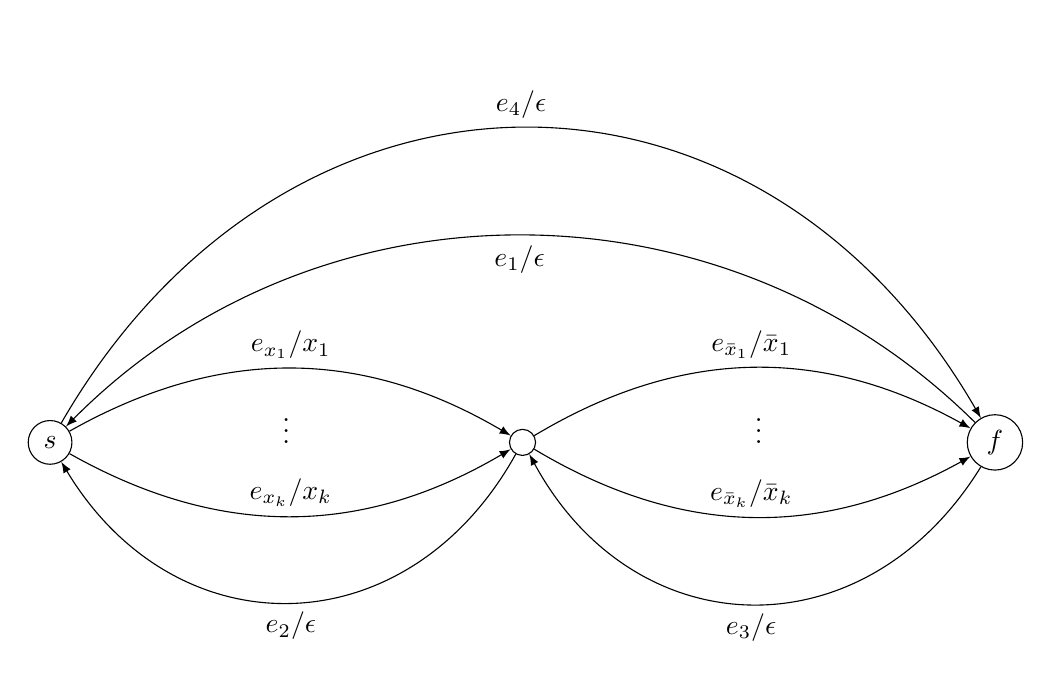
\begin{tikzpicture}
	\begin{pgfonlayer}{nodelayer}
		\node [style=state] (0) at (0, -0) {};
		\node [style=state] (1) at (-6, -0) {$s$};
		\node [style=state] (2) at (6, -0) {$f$};
		\node [style=none] (3) at (-3, 0.25) {$\vdots$};
		\node [style=none] (4) at (3, 0.25) {$\vdots$};
	\end{pgfonlayer}
	\begin{pgfonlayer}{edgelayer}
		\draw [style=transition, in=120, out=60, looseness=1.25] (1) to node[auto]{$e_4/\epsilon$} (2);
		\draw [style=transition, bend right=45, looseness=1.00] (2) to node[auto]{$e_1/\epsilon$} (1);
		\draw [style=transition, bend left, looseness=1.00] (1) to node[auto]{$e_{x_1}/x_1$} (0);
		\draw [style=transition, bend left, looseness=1.00] (0) to node[auto]{$e_{\bar{x}_1}/\bar{x}_1$} (2);
		\draw [style=transition, bend right, looseness=1.00] (1) to node[auto]{$e_{x_k}/x_k$} (0);
		\draw [style=transition, bend right, looseness=1.00] (0) to node[auto]{$e_{\bar{x}_k}/\bar{x}_k$} (2);
		\draw [style=transition, bend left=60, looseness=1.25] (0) to node[auto]{$e_2/\epsilon$} (1);
		\draw [style=transition, bend left=60, looseness=1.25] (2) to node[auto]{$e_3/\epsilon$} (0);
	\end{pgfonlayer}
\end{tikzpicture}
\end{center}

If we consider all labellings of paths from vertex $s$ to vertex $f$ we get of
course also words not contained in $D(X_k)$ like for example $x_1 x_2
\bar{x}_k$ or $x_1 \bar{x}_1 \bar{x}_2$ etc.

We have to guarantee that we get Dyck words only. 

To do that, we define a {\em homomorphism} from the paths of the graph into the
polycyclic monoid over $X_k \cup \bar{X}_k$ such that the homomorphic images of
the paths from $S$ to $F$ have a special form, for example are equal to the unit
of the polycyclic monoid.

If we consider the word $ x_1 x_2 \bar{x}_2 \bar{x}_1 x_2 \bar{x}_2 \in D(X_2)$
then we have different paths 
\[e_{x_1} e_2 e_{x_2} e_{\bar{x}_2} e_3 e_{\bar{x}_1} e_1 e_{x_2} e_{\bar{x}_2} \] 
and 
\[e_{x_1} e_2 e_{x_2} e_{\bar{x}_2} e_3 e_{\bar{x}_1} e_3 e_2 e_{x_2}
e_{\bar{x}_2}\] 
which both have this word as label and we can easily define a homomorphism in
the sense given above fulfilling the condition.

We get different paths in our graph leading to the acceptance of the same word.

The problem of constructing a graph such that for each word in the accepted
language exactly one path exists leads to the existence of the {\em
deterministic finite automaton with storage}.

\transrem{Finite automata with storage monoids have gained interest
in current research on computational algebra and automata theory, see for
example \cite{doi:10.1080/00927870802243580} and \cite{Render}.}

\chapter{Mathematical Foundations}
\section{Notations, basic terminology}

In this first section we want to define the elementary terminology that is used
throughout the whole book. We use the usual notations
\begin{eqnarray*}
\mathbb{N} &=& \setof{0, 1, 2, \ldots}\text{ for the natural numbers} \\
\mathbb{Z} &=& \setof{\ldots, -2, -1, 0, 1, 2, \ldots}\text{ for the integer
numbers} \\
\mathbb{Q} &=& \setof{\frac{a}{b} \mid a,b \in \mathbb{Z},\ b \neq 0}\text{
for the rational numbers}
\end{eqnarray*}

For the operations on sets we use $\cup$ for the union and $\cap$ for the
intersection. Also $A \subset B$, $a \in A$, $a \not\in A$, $\bar{A}$, $A - B$,
$A \times B$ and $\emptyset$ have their usual meaning.

For the power set of a set $A$ we write $\powset{A}$. $\card{A}$ denotes
the cardinality of $A$.

Logical implication is denoted by $\Rightarrow$.

{\bf Mappings} are denoted by $f : A \to B$ in which case $f$ is a
total mapping. We write $Q(f) = A,\ Z(f) = B$.\footnote{The letters $Q, Z$ stem 
from the German words ''Quelle'' (source) and ''Ziel'' (target).}

If $f: A \to B,\ g : B \to C$ are mappings, then $f \circ g : A
\to C$ is the {\bf composition} which one gets by applying $f$ first and then 
$g$:
\[(f \circ g)(a) = g(f(a))\]

If $f:A \to B$ and $C \subset A$, then $f(C) = \setof{f(c) \mid c \in C }$.

A subset $R \subset A \times B$ is called a {\bf relation} between $A$ and $B$.
\[R_f = \setof{(a,b) \mid b = f(a) } \subset A \times B\] 
is the relation {\bf induced by} the mapping f or also the {\bf graph} of $f$.

Let $f : A \to B$ be a mapping, $A_1 \subset A$ and $g : A_1 \to
B$ a mapping. 

$f$ is called the {\bf continuation} of $g$ if $f(a_1) = g(a_1),\ a_1 \in A_1$.
In this case we also write $f \mid _{A_1} = g$, in words: $f$ {\bf restricted to} $A_1$.

A {\bf semi-group} consists of a set $M$ and an associative operation on that
set, usually denoted as a multiplication. If a semi-group is commutative, we
also use ''$+$'' instead of ''$\cdot$''.

\index{monoid}
A semi-group is a {\bf monoid} if $M$ contains a neutral element. We often
denote the neutral element with $1_M$ or shortly $1$. In the commutative case we
often write $0$ instead of $1$.

For $A,B \subset M$ we denote by 
\[ A \cdot B = \setof{a \cdot b \mid a \in A,\ b \in B }\]
the {\bf complex product} of $A$ and $B$.

A subset $A \subset M$ is a {\bf submonoid} of $M$ if $1_M \in A$ and $A$ is
closed under the operation of $M$.

For a set $A$, the set $A^*$ is the smallest submonoid of $M$ containing $A$.
More specific, 
\[ A^* = \bigcap_{U \in M(A)} U	\]
where 
\[ M(A) = \setof{U \subset M \mid U \text{ is a submonoid of } M, A \subset U } \]

It is easy to see that
\[ A^* = \bigcup_{n \geq 0} A^n \text{ with }A^0 = \setof{1}\text{ and }A^{n+1}= A^n \cdot A \]

In the same sense the notion $A^+ = A^* - \setof{1}$ is defined for semi-groups.
$A$ is called the {\bf generating system} of $A^*$ and $A^+$ resp.

A special meaning for us has the set of {\bf words} ({\bf strings}) over
a fixed alphabet $A$. We understand as words the finite sequences of elements from
the alphabet $A$, for example $(a,b,d,a,c)$ over the alphabet $A = \setof{a,b,c,d
}$.

We define
\[ WORD(A) := \setof{\epsilon} \cup A \cup (A \times A) \cup (A \times A \times
A) \cup \ldots \]
as the {\bf set of words (strings) over} $A$. 

The symbol $\epsilon$ denotes the {\bf empty word} over $A$, that is $A^0 =
\setof{\epsilon}$.

If $v, w \in WORD(A)$ then $v \cdot w$ is the word which you get by
concatenating $v$ and $w$, formally:
\[ v = (a_1,\ldots, a_k),\ w = (a_{k+1}, \ldots, a_n) \Rightarrow v \cdot
w = (a_1, \ldots, a_n) \]

With this operation, $WORD(A)$ becomes a monoid which is usually also denoted
by $A^*$.

This naming is slightly inconsistent because for the first definition of
the $*$-operator it holds $(A^*)^* = A^*$, but for the second usage of the
$*$-operator it holds $(A^*)^* \neq A^*$.

The following example should clarify this fact: 

Let $A = \setof{a,b,c}$ and let $(a,b,a)$ and $(b,a) \in A^*$.
\[(a,b,a)\cdot(b,a) = (a,b,a,b,a) \in A^* \]
\[((a,b,a),(b,a)) \in (A^*)^*\text{, but }\notin A^* \]

Instead of $(a)$ we just write $a$. In this sense it holds $A \subset A^*$. This
also holds in the sense of the first definition of $A^*$.

If $w = (w_1, \ldots, w_n)$ we call $|w| := n$ the {\bf length} of $w$.
Obviously \[|w \cdot v| = |w| + |v|\text{ and }|\epsilon| = 0\]

(Later in this book, the notation $|w|$ is mainly used for reduced words and
the string length is then denoted by $\strlen{w}$.)

The {\bf reverse} of a word $w = (w_1,\ldots,w_n)$ is the word $w^R =
(w_n,\ldots,w_1)$. It holds:
\[ (w \cdot v)^R = v^R \cdot w^R \text{ and }\epsilon^R = \epsilon \]

In $A^*$ the {\bf cancellation rules} hold:
\begin{enumerate}
  \item $w \cdot x = w \cdot y \Rightarrow x = y$
  \item $x \cdot w = y \cdot w \Rightarrow x = y$
\end{enumerate}

We define {\bf left} and {\bf right quotient}:
\[ X^{-1} \cdot Y = \setof{w \mid \exists x \in X,\ y \in Y\text{ with }x \cdot w
= y } \] 
and 
\[ X \cdot Y^{-1} = \setof{w \mid \exists x \in X,\ y \in Y\text{ with } w \cdot y
= x } \]

Because of the cancellation rules it holds: $\setof{w}^{-1} \cdot \setof{v}$ and
$\setof{w}^{-1} \cdot \setof{v}$ are either empty or contain a single element.

If $\setof{w}^{-1} \cdot \setof{v}$ is not empty, we call $w$ a {\bf prefix} of $v$,
if $\setof{w} \cdot \setof{v }^{-1} \neq \emptyset$, we call $v$ a {\bf suffix}
of $w$.

In the future we will also just write $w$ instead of $\setof{w}$ and $w$ {\bf is
prefix of} $v$, if $w^{-1} \cdot v \neq \emptyset$.

\section{Monoid homomorphisms and congruence relations}

\begin{definition}
A {\bf monoid homomorphism} (short: homomorphism) from a monoid $M$ to a monoid
$S$ is a mapping $\phi : M \to S$ with:
\begin{enumerate}
  \item $\phi(m_1 \cdot m_2) = \phi(m_1) \cdot \phi(m_2), \quad m_1, m_2 \in M$
  \item $\phi(1_M) = 1_S$
\end{enumerate}
\end{definition}

\transrem{Some publications use even shorter just {\em morphism} but here this
would lead to a conflict with the morphisms in categories.}

It can be easily shown: if $U \subset M$ is a submonoid of $M$, then
$\phi(U)$ is a submonoid of $S$. If $V$ is a submonoid of $S$, then
$\phi^{-1}(V)$ is a submonoid of $M$.

A monoid homomorphism $\phi: M \to S$ is called
\begin{eqnarray*}
\text{\bf monomorphism} & & \text{ if $\phi$ is injective} \\
\text{\bf epimorphism} & & \text{ if $\phi$ is surjective} \\
\text{\bf isomorphism} & & \text{ if $\phi$ is bijective} \\
\text{\bf endomorphism} & & \text{ if $\phi: M\to M$} \\
\text{\bf automorphism} & & \text{ if $\phi$ is endomorphism and isomorphism} \\
\end{eqnarray*}
Monoids $M$ and $S$ are called {\bf isomorphic}, if there exists an
isomorphism between $M$ and $S$.

Of course, a homomorphism cannot be defined arbitrarily on a monoid $M$.
Thus the following two questions arise:
\begin{enumerate}
  \item If $U \subset M$ is a submonoid and $\phi_1 : U \to S$ is an arbitrary
mapping. When is it possible to extend $\phi_1$ to a homomorphism $\phi
: M \to S$\ ?
	\item If $\phi_1, \phi_2$ both are homomorphisms from $M$ to $S$ which
	coincide on $U \subset M$. In which way can $\phi_1$ and $\phi_2$ be
	different? 
\end{enumerate}

The answer to this question of course depends on the structure of $U$. If
$U = \{ 1_M \}$ then $\phi$ is determined uniquely on $U$ but there is
little information on the relation between $\phi_1$ and $\phi2$.

The following two simple theorems which can be found in introductory algebra
books hold:
\begin{enumerate}
  \item If $A$ is a generating system of $M$ and $\phi_1, \phi_2 : M \to S$ are
  monoid homomorphisms which coincide on $A$, then $\phi_1 = \phi_2$.
  \item If $A$ is a set, $M = A^*$, and $\phi_1 : A \to S$ is an arbitrary
  mapping, then there exists a unique continuation $\phi$ of $\phi_1$ which is
  a monoid homomorphism from $A^*$ to $S$.
\end{enumerate}

\begin{definition}
A subset $A \subset M$ is called a {\bf free generating system} of $M$, if each
mapping $\phi_1 : A \to S$, where $S$ is an arbitrary monoid, can be continued
to a monoid homomorphims in a unique way. 

A monoid with a free generating system is called a {\bf free monoid}.
\end{definition}

$A^*$ therefore is a free monoid and $A$ is a free generating system of $A^*$.

It holds too: If $A$ is a free generating system of $M$ and $A^*$ is the monoid
of words (string) over $A$, then $A^*$ and $M$ are isomorphic.

A free monoid has at most one free generating system (exercise. From that one
can see that the length $|w|$ of a word $w \in A^*$ can be defined in a unique way for any
free monoid.

The length function $L$ is an example for a monoid homomorphism $L : A^* \to
\mathbb{N}$.

If $\phi : M \to S$ is a monoid homomorphism, then the sets 
\[\{ \phi^{-1}(s) \mid s \in S \} \subset Pot(M) \]
form a monoid isomorphic to $\phi(M)$ (exercise).

We want to investigate now the following problem:

Let $M$ be a monoid, $L \subset M$ be any subset of $M$. Does there exist a
monoid $S$ and a homomorphism $\phi : M \to S$ with the following property:
There exists an $s \in S$ with $L \subset \phi^{-1}(s)$?

Of course, there always exists such an $S$: Choose $S = \{ 1 \}$ and $\phi(M) =
\{1\}$. Therefore we strengthen our task: 

Find $S$ and $\phi$ such that $L \subset \phi^{-1}(S)$ and for each other
homomorphism $\Psi$ with that property holds:
\[ L \subset \Psi^{-1}(S') \Rightarrow \phi^{-1}(S) \subset \Psi^{-1}(S') \]

We want to describe $L$ as close as possible by a monoid homomorphism.

Such an $S$ and $\phi$ exists for each $L \subset M$ (see Algebra text), it is
named $synt_M(L)$ an is constructed as follows:

\begin{definition}
Let $M$ be a monoid and $L \subset M$. For $a, b \in M$ we define
\[ a \equiv b (L) \iff \text{for all }u, v \in M: u \cdot a \cdot v \in L
\Leftrightarrow u \cdot b \cdot v \in L \]
\end{definition}

$\equiv (L)$ is a congruence relation, it holds:
\begin{enumerate}
  \item Let $[a]_L = \{ b \in M \mid a \equiv b\ (L) \}$\ then\ $b \in [a]_L
  \Rightarrow [a]_L = [b]_L $
  \item If we define $[a]_L \cdot [b]_L := [a \cdot b]_L$\ (complex product),
  then \[synt_M(L) = \{ [a]_L \mid a \in M \}\] becomes a monoid under this
  operation and the mapping \[\phi_L : M \to synt_M(L),\ \phi_L(a) = [a]_L\]
   is a monoid epimorphism.
\end{enumerate}

We call $\equiv (L)$ the {\bf syntactic congruence} of $L$ and $synt_M(L)$ the
{\bf syntactic monoid} of $L$ with respect to $M$.

To motivate the name {\em syntactic monoid} we give an example from German
language.

Let $A$ be the alphabet of German and $L$ the set of sentences in German. One can
denote two words $w_1$ and $w_2$ as congruent if they can always be exchanged in
each german sentence. There exist words that cannot always be exchanged. In the
sentence ''Apfel ist eine Kernfrucht'' the word ''Apfel'' can be exchanged by
''Birne'' but this is not possible in the sentence ''Apfel schreibt sich A p f e
l''.

The difficulty is of semantic nature. If you don't consider semantic correctness
of sentences you get a classification of words wrt. their syntactic meaning.

\transrem{I fear this example makes not a lot of sense in this translation}

The important notion of ''syntactic congruence'' has been introduced by M.\ P.\
Schützenberger in the context of coding problems.

{\bf Exercise:} Prove the following 
\begin{theorem}
It is decidable if a monoid homomorphism $\alpha$ is injective.
\end{theorem}

Hint: Let $\alpha: A^* \to B^*$ be a given monoid homomorphism, $A =
\{a_1,\ldots,a_n\},\ E = \{\alpha(a_1),\ldots,\alpha(a_n)\}$.

Consider $A_1 := \{ u^{-1} v \in B^* \mid u, v \in E,\ u\neq v \}$ and then
inductively $A_{k+1} = A_k^{-1} E \cup E A_k$.

Prove that
\begin{enumerate}
  \item The construction of the $A_k$ halts
  \item $1 \in \cup A_k \iff \alpha\text{ is not injective}$.
\end{enumerate}


\begin{corollary}
In a free monoid it is decidable if a finite set is a free generating system.
\end{corollary}

\section{Special monoids and the free group}

We have just learned about the syntactic monoid as an example for a monoid. For
the theory of syntactic monoids see \cite{Salomaa} and \cite{Perrot}.

Let's have a look at other special monoids which we will need again later. To do
so, we introduce the notion of a {\bf generated congruence relation}.

Let $A$ be an alphabet and
\[ R = \setof{u_i = v_i \mid i = 1, \ldots, n,\ u_i, v_i \in A^*} \] 
a set of equations.

Then by the following conditions a congruence relation $\bar{R}$ is uniquely
determined (exercise):
\begin{enumerate}
  \item $\setof{(u_i, v_i) \mid u_i = v_i \in R} \subset \bar{R}$
  \item $\bar{R}$\ is a congruence relation
  \item $\bar{R} \subset R'$\ for all $R'$\ fulfilling (1) and (2).
\end{enumerate}

$\bar{R}$ is the smallest congruence relation in which all
the equations from $R$ hold and is called the congruence relation 
{\bf generated by} $R$ on $A^*$.

The factor monoid $A^*/\bar{R}$ will also simply be named $A^*/R$. It holds:

Two words $u, v \in A^*$ are congruent modulo $\bar{R}$ (notation: $u
\equiv v (\bar{R})$) iff there exists $n \in \mathbb{N},\ u_i \in A^*$ with $u_i
= u_i' \cdot u_i \cdot u_i''$ such that for $i = 1, \ldots, n$:
\begin{enumerate}
  \item $u = u_1,\ v = u_n$
  \item $u_i' = u_{i+1}',\ u_{i}'' = u_{i+1}'',\ (u_{i} = u_{i+1}) \in R$ 
  for $i = 1, \ldots, n-1$.
\end{enumerate}

We say: $v$ is constructed from $u$ by {\bf applying the equations} from $R$.

The congruence classes of $u \in A^*$ in the factor monoid $A^*/R$ are denoted
by $[u]_{A^*/R}$ or simply $[u]$.

\begin{definition}
Let $X$ be an alphabet. Define $X^{-1} := \setof{x^{-1} \mid x \in X}$ as the
set of formal inverses.
\end{definition}

We can think of $x$ and $x^{-1}$ as corresponding pairs of
brackets as we did in the definition of the Dyck languages in the introduction.

We will now introduce a partition of $(X \cup X^{-1})^*$ wrt.\ to
different congruence relations and look into the corresponding factor monoids.

\begin{definition}
\[ \hgroup{X} := (\unioninv{X})^*\ /\ \setof{x x^{-1} = 1 \mid x \in X} \] is
called the {\bf H-group}\footnote{In the literature this monoid (which is not a
group!) is also called {\em free half-group} or {\em involutive monoid}.}.
\end{definition}

We introduce a special absorbing element $0$ by defining:
\begin{definition}
\begin{eqnarray*}
\pocymon{X} & := & (\unioninv{X} \cup \setof{0})^*\ /\ \\
& & \setof{x x^{-1} = 1,\,x y^{-1} = 0,\,0 z = z 0 = 0 \mid x,y \in X,\ x\neq
y,\ z \in \unioninv{X} \cup \setof{0}}
\end{eqnarray*}
is called the {\bf polycyclic monoid}.
\end{definition}

Using the naming of the previous section we get:
\[ \pocymon{X} = synt_{X^*}(D(X)) \]
which means:

The polycyclic monoid is the syntactic monoid of the Dyck language (exercise).

\begin{definition}
\[ F(X) := (\unioninv{X})^*\ /\ \setof{x \cdot x^{-1} = x^{-1} \cdot x = 1 \mid
x \in X} \]
\end{definition}
is the {\bf free group} over $X$.

\label{dyck-language}
Remark: It holds $D(X) = [1]_{\pocymon{X}}$ and $D(X) = [1]_{\hgroup{X}}$ which
means the Dyck language is the set of words from $(\unioninv{X})^*$ which can be
reduced to the empty word either using the equations of the H-group or the
equations of the polycyclic monoid.

In the following we will mainly consider \hgroup{X}, the H-group over $X$.

For $w \in (\unioninv{X})^*$ we define the reduced word $|w|$ as follows: 

If $w$ does not contain a subword of the form $x x^{-1}$ then $|w| := w$.
Otherwise, iteratively replace the leftmost occurence of the subword $x
x^{-1}$ by 1.

This process is called {\bf reduction} and the result is denoted by $\rho(w)$.

One can easily prove:

\begin{lemma}
There exists a minimal number $k \in \mathbb{N}$ with $\rho^k(w) = |w|$. This
number is called the {\bf reduction length}. It holds $\rho(|w|) = |w|$.
\end{lemma}

\bigskip
\begin{lemma}
For $[w], [w'] \in \hgroup{X}$ holds:
\[ [w] = [w'] \iff |w| = |w'| \]
\end{lemma}

\begin{proof}
''$\Leftarrow$'': It holds $w \equiv |w| = |w'| \equiv w' \Rightarrow [w] =
[w']$.

''$\Rightarrow''$: Let $[w] = [w']$. We may assume that $w'$ is created from $w$
by application of an equation $x x^{-1} = 1$. Let $w = w_1 x x^{-1} w_2$ and $w' = w_1 w_2$.

We show: If $k$ is the reduction length of $w_1$, then $\rho^{k+1}(w) =
\rho^k(w')$\ (thus the reduced words are equal).

Proof by induction over $k$:
\begin{itemize}
  \item  $k = 0$: $w_1$ is already reduced, so $\rho(w) = w_1 w_2 = w'$.
  \item $k > 0$: It holds $\rho(w) = \rho(w_1 x x^{-1} w_2),\ \rho(w') = \rho(w_1
w_2)$. The reduction length of $\rho(w)$ by induction assumption is $k-1$ and
$\rho^k \rho(w) = \rho^{k-1}\rho(w') \Rightarrow$ the reduced word of $w$ and
$w'$ is the same so $|w| = |w'|$.
\end{itemize}
\end{proof}

Remark: Using the same argument one can show that the creation of the reduced
word does not depend on the order of the reductions. Therefore the reduced word
for a representative of an element of $\hgroup{X}$ is unique, so we can speak of {\em the} 
reduced word in the following.

Remark: These results have been used in \cite{HotzMesserschmidt} to obtain a
space-optimal algorithm for the analysis of the Dyck language.

Similar results also hold for the free group $F(X)$, see \cite{CrowellFox}.

\section{Graphs, categories and functors}

Before defining graphs formally we want to explain informally what we mean by a
graph. A graph consists of points and edges. Each edge connects two points which
are not necessarily different. You can imagine a graph as streetmap, the cities
are the points and the streets are the edges of the graph. The edges may be
oriented such that they have a one-way direction. Paths in graphs are sequences
of edges that you could drive for example with a car without violating the
traffic rules.

One can show that every graph, as we will formally define it, possesses (with a
certain restriction) a faithful image in $\mathbb{R}^3$, see e.g.\
\cite{Wagner}. The points of the graph become points in $\mathbb{R}^3$, the
edges become connecting lines in $\mathbb{R}^3$ which pairwise do not intersect.

The restriction concerning the points of the graph is that the graph must not
have more points than there exist in $\mathbb{R}^3$ (cardinality of the
continuum).

The restriction concerning the edges is more essential: It tells that there is
at most one edge between two points and that the graph has no loops. Loops are
edges with just a single border point.

From what has been said we see that we may use a concrete geometric imagination
of a graph without getting our intuition mistaken. The following definition of a
graph nevertheless does not contain any geometry.

\bigskip
\begin{definition}
A {\bf graph} $G = (V, E)$ consists of a non-empty set $V$ of vertices (points),
a set $E$ of edges and a mapping 
\[ \rho: E \to \powset{V}\text{ with }\card{\rho(e)} <= 2\text{ for }e \in E \]
$\rho(e)$ is the set of {\em border points} of $e$.
\end{definition}

The border points of an edge do not need to be different. If $\card{\rho(e)} =
2$ we call $e$ a {\bf line}, if $\card{\rho(e)} = 1$ we call it a {\bf loop}.

\bigskip
\begin{definition}
A graph is called {\bf loop-free} if it does not contain any loops.
\end{definition}

We introduce an orientation for the edges. 

\begin{definition}
A graph $G = (V,E)$ is called {\bf oriented graph} if there are two mappings
$Q : E \to V$ and $Z : E \to V$ with
\[ \rho(e) = \setof{Q(e), Z(e)}\text{ for all }e \in E \]
\end{definition}

$Q(e)$ is called the {\bf source vertex} and $Z(e)$ the {\bf target vertex} of
$e$ \footnote{The letters $Q$ and $Z$ stem from the German words for source
(''Quelle'') and target (''Ziel'').}.

The notions of loop and line are naturally transferred to oriented graphs.

To each graph one can assign the corresponding oriented graph $\hat{G}$ by
defining two edges
\[ (v_1, e, v_2)\text{ and }(v_2,e,v_1) \]
for each edge $e$ with border points $v_1$ and $v_2$ and defining
\begin{eqnarray*}
& Q((v_1, e, v_2)) = v_1 = Z((v_2, e, v_1)) \\
& Q((v_2, e, v_1)) = v_2 = Z((v_1, e, v_2))
\end{eqnarray*}

\bigskip
\begin{definition}
A graph $G = (V,E)$ is called {\bf connected} if in the corresponding oriented
graph $\hat{G}$ for each pair of points $v$ and $v'$ there exist edge sequences
$e_1, \ldots, e_k$ with
\[ Q(e_1) = v,\ Z(e_k) = v'\text{ and }Z(e_i) = Q(e_{i+1})\text{ for }i = 1,
\ldots, k-1 \]
\end{definition}

\bigskip
\begin{definition}
A loop-free graph $G = (V,E)$ is called {\bf ordered} if for each point $v \in
V$ holds:

There exists a unique (up-to cyclic permutation) ordering on the set
\[ \mathrm{cycle}(v) := \setof{e \in E \mid v \in \rho(e)} \]
\end{definition}

The set $\mathrm{cycle}(v)$ is called the {\bf cycle} that belongs to $v$.

Explanation: Imagine each point and its adjacent edges to be stuck on a litte
disk as shown in the following figure:

\begin{center}
\begin{tikzpicture}
	\begin{pgfonlayer}{nodelayer}
		\node [style=none] (0) at (0, -0) {};
		\node [style=none] (1) at (-2, 3) {};
		\node [style=none] (2) at (2, 3) {};
		\node [style=none] (3) at (3, -2) {};
		\node [style=none] (4) at (-2, -2) {};
		\node [style=none] (5) at (-3, 1) {};
	\end{pgfonlayer}
	\begin{pgfonlayer}{edgelayer}
		\draw (1.center) to node[auto]{$e_1$} (0.center);
		\draw (2.center) to node[auto]{$e_2$} (0.center);
		\draw (3.center) to node[auto]{$e_3$} (0.center);
		\draw (4.center) to node[auto]{$e_4$} (0.center);
		\draw (5.center) to node[auto]{$e_5$} (0.center);
	\end{pgfonlayer}
\end{tikzpicture}
\end{center}

In this figure the orderings for $\setof{e_1, e_2, e_3, e_4, e_5}$ are:
\begin{eqnarray*}
& e_1, e_2, e_3, e_4, e_5 \\
& e_2, e_3, e_4, e_5, e_1 \\
& \vdots & \\
& e_5, e_1, e_2, e_3, e_4
\end{eqnarray*}

\bigskip
\begin{definition}
A loop-free, oriented graph $G$ is called {\bf ordered} if for all points
$v \in V$ it holds: 

In the cycle of $v$ there exists an ordering 
\[ e_1, \ldots, e_k, e_m', \ldots, e_1'\]
such that
\[ \setof{e_1, \ldots, e_k} = \setof{e \in E \mid Z(e) = v} \]
and 
\[ \setof{e_1', \ldots, e_m'} = \setof{e \in E \mid Q(e) = v} \]
\end{definition}

$e_1, \ldots, e_k$ is called the {\bf ordering} of the incoming edges of $v$ and
$e_1', \ldots, e_m'$ the ordering of the outgoing edges of $v$.

\medskip
{\bf Example:}

\begin{center}
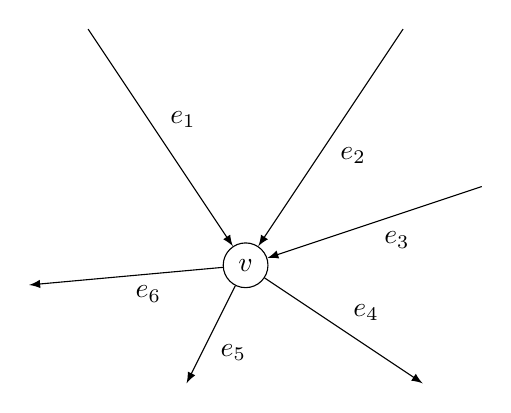
\begin{tikzpicture}
	\begin{pgfonlayer}{nodelayer}
		\node [style=state] (0) at (0, -0) {$v$};
		\node [style=none] (1) at (-2, 3) {};
		\node [style=none] (2) at (2, 3) {};
		\node [style=none] (3) at (3, 1) {};
		\node [style=none] (4) at (2.25, -1.5) {};
		\node [style=none] (5) at (-0.75, -1.5) {};
		\node [style=none] (6) at (-2.75, -0.25) {};
	\end{pgfonlayer}
	\begin{pgfonlayer}{edgelayer}
		\draw [style=transition] (1.center) to node[auto]{$e_1$} (0);
		\draw [style=transition] (2.center) to node[auto]{$e_2$} (0);
		\draw [style=transition] (3.center) to node[auto]{$e_3$} (0);
		\draw [style=transition] (0) to node[auto]{$e_4$} (4.center);
		\draw [style=transition] (0) to node[auto]{$e_5$} (5.center);
		\draw [style=transition] (0) to node[auto]{$e_6$} (6.center);
	\end{pgfonlayer}
\end{tikzpicture}
\end{center}

$e_1, e_2, e_3, e_4, e_5, e_6$ is the ordering of vertex $v$.

$e_1, e_2, e_3$ is the ordering of the incoming edges.

$e_6, e_5, e_4$ is the ordering of the outgoing edges.

\bigskip
\begin{definition}
A {\bf path} in an oriented graph $G$ is a sequence 
\[ \pi = (q, e_1, \ldots, e_k, z),\ k \geq 1 \]
where $ e_1, \ldots, e_k \in E$ are edges and
\begin{eqnarray*}
Q(e_1) & = & q \\
Z(e_{i}) & = & Q(e_{i+1})\text{ for }i = 1, \ldots, k-1 \\
Z(e_k) & = & z 
\end{eqnarray*}
\end{definition}

We continue the source and target mappings $Q$ and $Z$ onto paths by defining
\[ Q(\pi) := q,\quad Z(\pi) := z \]
$q$ is called the {\bf start point} and $z$ the {\bf end point} of $\pi$.

$\len{\pi} := k$ is called the {\bf length} of the path $\pi$. For $k = 0$ we
define for all points $v \in V$ that $\pi = (v, v)$ is the path of length 0 from
$v$ to $v$.

Paths in arbitrary graphs are defined by turning to the oriented graph
$\hat{G}$.

\bigskip
\begin{definition}
Let $\pi = (q, e_1, \ldots, e_k, z)$ be a path. A path $\pi' = (q', e'_1,
\ldots, e'_m, z')$ is called a {\bf subpath} of $\pi$ if there exists an $i$
with $1 \leq i \leq k$ such that
\[ e'_j = e_{i+j-1},\ j = 1, \ldots, m,\ i + m - 1 \leq k \]
\end{definition}

A path is called {\bf closed} if $Q(\pi) = Z(\pi)$, it is called a {\bf circle}
if it is closed and does not contain any closed subpath $\pi'$ with $\len(\pi')
> 0$.

\bigskip
\begin{definition}
A graph $G = (V, E)$ is called {\bf circle-free} if there are no circles in $G$.
\end{definition}

For our purposes we will only consider oriented graphs. For these graphs the
following definition reflects a special connectivity property.

\begin{definition}
Let $G = (V, E)$ be an oriented graph and $c \in V$. $G$ is called a {\bf star
relative to $c$} if for each $v \in V$ there exists a path $\pi_{v}$ with
$Q(\pi_{v}) = c$ and $Z(\pi_{v}) = v$. $c$ is called the {\bf center} of $G$.
\end{definition}

We want to introduce now a special kind of graph that plays a central role in
the theory of formal languages.

\begin{definition}
A {\bf tree} is a circle-free star where for all $v \in V$ it holds
\[ \card{\setof{e \in E \mid Z(e) = v}} \leq 1 \]
\end{definition}

The following lemma holds:
\begin{lemma}
A tree has exactly one center (called {\bf root}).
\end{lemma}

Historical remark: Leonard Euler (1735) at a walk in Königsberg asked himself if
he could walk in such a way that he would traverse each of the seven bridges
over the Memel river exactly once. In the figure below you can see a graph
describing the situation. Euler stated a simple condition for the existence of
paths that traverse each edge of a graph exactly once ({\em Euler paths}).

\begin{center}
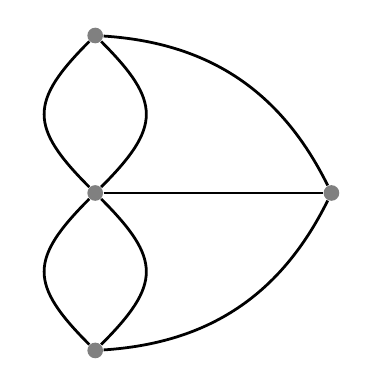
\begin{tikzpicture}
	\begin{pgfonlayer}{nodelayer}
		\node [style={filled_vertex}] (0) at (0, -0) {};
		\node [style={filled_vertex}] (1) at (0, 2) {};
		\node [style={filled_vertex}] (2) at (0, -2) {};
		\node [style={filled_vertex}] (3) at (3, -0) {};
	\end{pgfonlayer}
	\begin{pgfonlayer}{edgelayer}
		\draw [style=simple] (0) to (3);
		\draw [style=simple, bend right=45, looseness=1.50] (0) to (2);
		\draw [style=simple, bend left, looseness=1.00] (3) to (2);
		\draw [style=simple, bend right, looseness=1.00] (3) to (1);
		\draw [style=simple, bend left=45, looseness=1.50] (0) to (1);
		\draw [style=simple, bend left=45, looseness=1.50] (1) to (0);
		\draw [style=simple, bend left=45, looseness=1.50] (0) to (2);
	\end{pgfonlayer}
\end{tikzpicture}
\end{center}

We want to {\em concatenate} paths, we define the {\em product of paths}:
\[ (q, e_1, \ldots, e_k, z) \cdot (q', e_{k+1}, \ldots, e_n, z') := (q, e_1,
\ldots, e_n, z')\text{ if } z = q' \]

That means you can concatenate two paths if the end point of the first path is
the start point of the second path.

Obviously it holds:
\begin{enumerate}
\item The product of paths (if defined) is associative
\item For each point $v$ of a graph $G$ there exists exactly one path $1_v :=
(v, v)$ such that for each path $\pi$ it holds:
	\begin{eqnarray*}
  	\pi \cdot 1_v = \pi\quad\text{if }Z(\pi) = v \\
  	1_v \cdot \pi = \pi\quad\text{if }Q(\pi) = v
	\end{eqnarray*}
\end{enumerate}

We denote the set of paths of a graph $G$ with $\pathcat{G}$. 
$\pathcat{G}$\footnote{The letter
$\mathfrak{W}$ stems from the German word ''Wegekategorie'' (path category).} 
is called the {\bf path category} of $G$ and in this context $G$ is also called 
a {\bf schema}. $\pathcat{G}$ is an important special case of a {\em category}.

Notation: 
\[ \pathcat{G}(v, v') := \setof{\pi \in \pathcat{G} \mid Q(\pi) = v,\ Z(\pi) =
v'} \]

\bigskip
Categories are algebraic structures with a {\em partial} operation.

\begin{definition}
$C = (O, M, Q, Z, \circ)$ is called a {\bf category} if the axioms (K1) to
(K4) hold:
\begin{enumerate}
	\item[(K1)] $O$ and $M$ are sets and $Q: M \to O$ and $Z: M \to O$ are
	mappings.\\
	$Q(f)$ is the {\bf source} of $f$ and $Z(f)$ is the {\bf target} of $f$.\\
	$O$ is the set of {\bf objects} and $M$ the set of {\bf morphisms} of the
	category $C$.
	
	\item[(K2)] For morphisms $f, g \in M$ the operation $\circ$ is defined
	exactly if $Q(g) = Z(f)$. In this case it holds $f \circ g \in M,\ Q(f \circ g)
	= Q(f),\ Z(f \circ g) = Z(g)$.
	
	\item[(K3)] The associative law $f \circ (g \circ h) = (f \circ g) \circ h$
	holds in the sense that each of both sides is defined if one of them is.
	
	\item[(K4)] For each object $w \in O$ there exists a {\em unit morphism} $1_w
	\in M$ with $Q(1_w) = Z(1_w) = w$ and for all morphisms $f, g \in M$ with 
	$Q(f) = Z(g) = w$ holds:
	\[ 1_w \circ f = f\text{ and }g \circ 1_w = g \]
	It can easily be shown that there exists exactly one unit morphism for each
	object $w$.
\end{enumerate}
\end{definition}

Notations: $Obj(C) := O$ is called the {\bf set of objects} and $Mor(C) := M$
the {\bf set of morphisms} of the category $C$.

Historical remark: Already Euler was interested in graphs and paths in
graphs (see above). The path category of a graph had already been used
before the notion of a {\em category} even existed.

The axiomatic formulation of categories and its importance for many areas of
mathematics has been elaborated by S.\ Eilenberg and S.\ MacLane in 1945
\cite{EiMa}. Their work produced a broad, very abstract theory of categories. We
will use here only the notations for structures which are categories and some 
elementary concepts which also in the theory of formal languages lead to 
fruitful questions.

We explain the notion of a category with some examples:
\begin{enumerate}
  \item {\bf The category of relations}
  
  Let $O$ be a set of sets ($O \notin O)$. Define 
  \[ \mathrm{REL}(O) := (O, M, Q, Z,\circ) \] by:
  \begin{itemize}
  	\item[] $M := \setof{(A,B,R) \mid A \in O,\ B \in O,\ R \subset A \times B}$
  	\item[] $Q(A,B,R) := A, \ Z(A,B,R) := B$
  	\item[] $(A,B,R_1) \circ (B,C,R_2) := (A,C,R')\\
  	\text{where }R'= \setof{(a, c) \mid \exists\, b \in B: (a, b)\in R_1\text{
  	and }(b, c)\in R_2}$
  \end{itemize}
  With these definitions $\mathrm{REL}(O)$ becomes a category (exercise). The
  morphisms $(A, A, \setof{(a, a) \mid a \in A})$ are the units for each set $A
  \in O$.

  \item {\bf The category of matrices}
  
  Define 
  \[ \mathrm{MAT}(\mathbb{Q}) := (O. M, Q, Z, \circ) \]
  by:
  \begin{itemize}
    \item[] $O := \mathbb{N}$
    \item[] $M :=$ the set of $k \times n$-matrices with entries from
    $\mathbb{Q}\ (k, n \in \mathbb{N})$.
    \item[] For a $k \times n$-matrix $A_{k,n}$ define source and target
    mapping by
    \begin{itemize}
	    \item[] $Q(A_{k,n}) := k$ (the number of rows)
  	  \item[] $Z(A_{k,n}) := n$ (the number of columns)
    \end{itemize}
  \end{itemize}
	With the matrix multiplication as category operation $\circ$,
	$\mathrm{MAT}(\mathbb{Q})$ becomes a category. Units in this category are
	the $n\times n$ unit matrices, $n \in \mathbb{N}$.
\end{enumerate}

In analogy to the monoid homomorphisms we want to introduce
now structure-preserving mappings between categories called {\bf functors}.

\begin{definition}
Let $C_i = (O_i, M_i, Q_i, Z_i, \circ_i), i = 1, 2$ be two categories and
$\phi_1: O_1 \to O_2$ and $\phi_2: M_1 \to M_2$ mappings.
\[ \phi = (C_1, C_2, \phi_1, \phi_2) \]
is called a {\bf functor} from $C_1$ to $C_2$ if the axioms (F1) to (F3) hold:
\begin{itemize}
  \item[(F1)] The diagram
	\begin{tikzcd}[column sep=large,row sep=large]
	 O_1 \arrow[leftarrow]{r}{Q_1} \arrow{d}{\phi_1} & M_1 \arrow{r}{Z_1}
	 \arrow{d}{\phi_2} & O_1 \arrow{d}{\phi_1} \\
	 O_2 \arrow[leftarrow]{r}{Q_2} & M_2 \arrow{r}{Z_2} & O_2
	\end{tikzcd}
	is commutative.
  
  \item[(F2)] $\phi_2(f \circ_1 g) = \phi_2(f) \circ_2 \phi_2(g)$ for all $f, g
  \in M_1$ with $Z(f) = Q(g)$.
  
  \item[(F3)] $\phi_2(1_w) = 1_{\phi_1(w)}$ for all $w \in O_1$.
\end{itemize}
\end{definition}

A functor $\phi$ is called injective (surjective, bijective) if $\phi_1$ and
$\phi_2$ are injective (surjective, bijective).

Let's look at some examples:

\begin{example}
Consider the following oriented graphs $G_1$ and $G_2$:

$G_1$:
\begin{center}
\begin{tikzpicture}
	\begin{pgfonlayer}{nodelayer}
		\node [style=none] (0) at (0, -0) {};
		\node [style=none] (1) at (-2, -1) {};
		\node [style=none] (2) at (2, -1) {};
		\node [style=none] (3) at (-3, -2) {};
		\node [style=none] (4) at (-1, -2) {};
		\node [style=none] (5) at (1, -2) {};
		\node [style=none] (6) at (3, -2) {};
		\node [style=none] (7) at (-4, -3) {};
		\node [style=none] (8) at (4, -3) {};
	\end{pgfonlayer}
	\begin{pgfonlayer}{edgelayer}
		\draw [style=transition] (0.center) to node[auto]{$f$} (1.center);
		\draw [style=transition] (1.center) to node[auto]{$f$} (3.center);
		\draw [style=transition] (1.center) to node[auto]{$g$} (4.center);
		\draw [style=transition] (0.center) to node[auto]{$g$} (2.center);
		\draw [style=transition] (2.center) to node[auto]{$f$} (5.center);
		\draw [style=transition] (2.center) to node[auto]{$g$} (6.center);
		\draw [style=transition] (3.center) to node[auto]{$f$} (7.center);
		\draw [style=transition] (6.center) to node[auto]{$g$} (8.center);
	\end{pgfonlayer}
\end{tikzpicture}
\end{center}
$G_1 = (V_1, E_1)$ represents an infinite binary tree. From each point of the
tree two edges go out which are labelled with $f$ and $g$.

$G_2$:
\begin{center}
\begin{tikzpicture}[scale=8.0]
	\begin{pgfonlayer}{nodelayer}
		\node [style=state] (0) at (0, -0) {$v_0$};
	\end{pgfonlayer}
	\begin{pgfonlayer}{edgelayer}
		\draw [style=transition, in=135, out=-135, loop] (0) to node[auto]{$f$} ();
		\draw [style=transition, in=-45, out=45, loop] (0) to node[auto]{$g$} ();
	\end{pgfonlayer}
\end{tikzpicture}
\end{center}
$G_2 = (V_2, E_2)$ consists of a single point $v_0$ and two loops labeled $f$ and $g$ respectively.

Consider the path categories $\pathcat{G_1}$ and $\pathcat{G_2}$. For $v
\in V_1$ define $\phi_1(v) := v_0$ and $\phi_2(1_v) := 1_{v_0}$.

For the edges $e \in E_1$ define
\[ \phi'_2(e) = 
\begin{cases}
	f & \text{if $e$ is marked with $f$} \\ 
	g & \text{if $e$ is marked with $g$}
\end{cases} 
\]
Now we define for the paths $(v, e_1, \ldots, e_n, v') \in \pathcat{G_1}$:
\[ \phi_2((v, e_1, \ldots, e_n, v')) := (v_0, \phi'_2(e_1), \ldots,
\phi'_2(e_n), v_0) 
\]
Obviously $\phi = (\pathcat{G_1}, \pathcat{G_2}, \phi1, \phi_2)$ is a
functor. It is even a particular functor because
\begin{enumerate}
  \item $\phi$ is surjective
  \item If $v_1$ is a point in $G_1$ and $\bar{\pi}$ a path in $G_2$ then
  there exists exactly one path $\pi$ in $G_1$ with $Q(\pi) = v_1$ such that
  $\phi_2(\pi) = \bar{\pi}$.
\end{enumerate}
\end{example}

\bigskip
\begin{example}
Let graphs $G_1, G_2$ be given as follows:

$G_1$:
\begin{center}
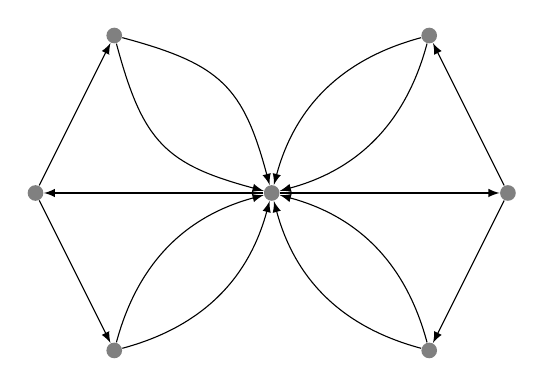
\begin{tikzpicture}
	\begin{pgfonlayer}{nodelayer}
		\node [style={filled_vertex}] (0) at (0, -0) {};
		\node [style={filled_vertex}] (1) at (-2, 2) {};
		\node [style={filled_vertex}] (2) at (2, 2) {};
		\node [style={filled_vertex}] (3) at (-2, -2) {};
		\node [style={filled_vertex}] (4) at (2, -2) {};
		\node [style={filled_vertex}] (5) at (-3, -0) {};
		\node [style={filled_vertex}] (6) at (3, -0) {};
	\end{pgfonlayer}
	\begin{pgfonlayer}{edgelayer}
		\draw [style=transition] (0) to (5);
		\draw [style=transition] (0) to (6);
		\draw [style=transition] (5) to (1);
		\draw [style=transition] (5) to (3);
		\draw [style=transition] (6) to (2);
		\draw [style=transition] (6) to (4);
		\draw [style=transition, bend left, looseness=1.25] (1) to (0);
		\draw [style=transition, bend right, looseness=1.25] (1) to (0);
		\draw [style=transition, bend right, looseness=1.00] (2) to (0);
		\draw [style=transition, bend left, looseness=1.00] (2) to (0);
		\draw [style=transition, bend right, looseness=1.00] (3) to (0);
		\draw [style=transition, bend left, looseness=1.00] (3) to (0);
		\draw [style=transition, bend left, looseness=1.00] (4) to (0);
		\draw [style=transition, bend right, looseness=1.00] (4) to (0);
	\end{pgfonlayer}
\end{tikzpicture}
\end{center}

$G_2:$
\begin{center}
\begin{tikzpicture}[scale=8.0]
	\begin{pgfonlayer}{nodelayer}
		\node [style=state] (0) at (0, -0) {$v_0$};
	\end{pgfonlayer}
	\begin{pgfonlayer}{edgelayer}
		\draw [style=transition, in=135, out=-135, loop] (0) to node[auto]{$f$} ();
		\draw [style=transition, in=-45, out=45, loop] (0) to node[auto]{$g$} ();
	\end{pgfonlayer}
\end{tikzpicture}
\end{center}
Then there exists a surjective functor from $\pathcat{G_1}$ to $\pathcat{G_2}$
(exercise).

It is possible to construct surjective functors which fulfill (2) from example 1
and other surjective functors which don't (exercise).
\end{example}

\bigskip
\begin{example}
Let $G_1$ and $G_2$ be given as:
\[ G_1:\ p_1 \edge{s} p_2 \qquad p_3 \edge{r} p_4 \]
\[ G_2:\ q_1 \edge{f} q_2 \edge{g} q_3 \]

We define:
\[ \phi_1(p_1) = q_1,\ \phi_1(p_2) = q_2,\ \phi_1(p_3) =
q_2,\ \phi_1(p_4) = q_3 \]
and
\[ \phi_2((p_1, s, p_2)) = (q_1, f, q_2),\ \phi_2((p_3, r, p_4)) = (q_2, g,
q_3)\]

For the units, the definition of $\phi_2$ is clear. One can see that 
\[ \phi = (\pathcat{G_1}, \pathcat{G_2}, \phi_1, \phi_2) \]
is a functor.

It is remarkable that $\phi_2(\pathcat{G_1})$ is not a category because this
set is not closed under the $\circ$ operation.
\end{example}

\bigskip
\begin{example}
Let $G_1$ and $G_2$ be given as follows:

$G_1$:
\begin{center}
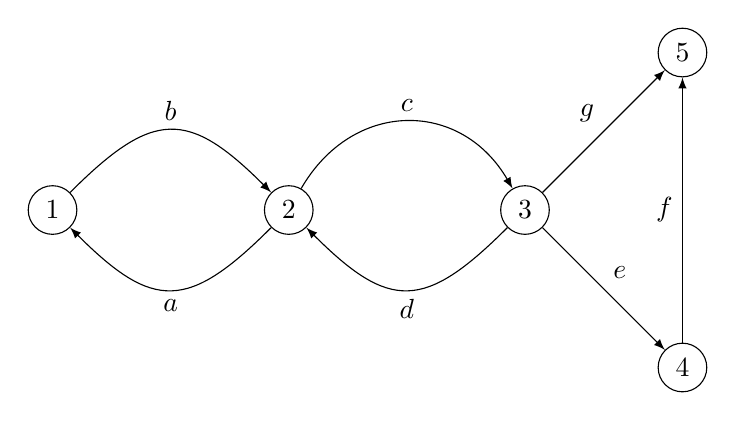
\begin{tikzpicture}
	\begin{pgfonlayer}{nodelayer}
		\node [style=state] (0) at (0, -0) {$1$};
		\node [style=state] (1) at (3, -0) {$2$};
		\node [style=state] (2) at (6, -0) {$3$};
		\node [style=state] (3) at (8, 2) {$5$};
		\node [style=state] (4) at (8, -2) {$4$};
	\end{pgfonlayer}
	\begin{pgfonlayer}{edgelayer}
		\draw [style=transition, bend left=45, looseness=1.50] (0) to node[auto]{$b$} (1);
		\draw [style=transition, bend left=45, looseness=1.50] (1) to node[auto]{$a$} (0);
		\draw [style=transition, bend left=60, looseness=1.25] (1) to node[auto]{$c$} (2);
		\draw [style=transition, bend left=45, looseness=1.50] (2) to node[auto]{$d$} (1);
		\draw [style=transition] (2) to node[auto]{$g$} (3);
		\draw [style=transition] (2) to node[auto]{$e$} (4);
		\draw [style=transition] (4) to node[auto]{$f$} (3);
	\end{pgfonlayer}
\end{tikzpicture}
\end{center}

$G_2$:
\begin{center}
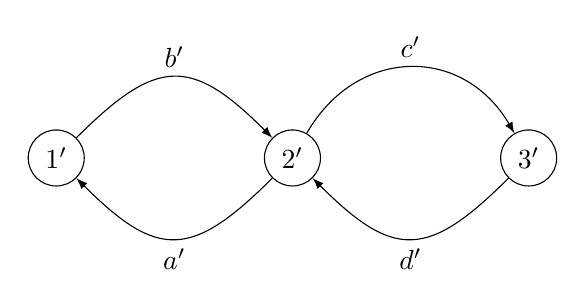
\begin{tikzpicture}
	\begin{pgfonlayer}{nodelayer}
		\node [style=state] (0) at (0, -0) {$2'$};
		\node [style=state] (1) at (-3, -0) {$1'$};
		\node [style=state] (2) at (3, -0) {$3'$};
	\end{pgfonlayer}
	\begin{pgfonlayer}{edgelayer}
		\draw [style=transition, bend left=45, looseness=1.50] (1) to node[auto]{$b'$} (0);
		\draw [style=transition, bend left=45, looseness=1.50] (0) to node[auto]{$a'$} (1);
		\draw [style=transition, bend left=60, looseness=1.25] (0) to node[auto]{$c'$} (2);
		\draw [style=transition, bend left=45, looseness=1.50] (2) to node[auto]{$d'$} (0);
	\end{pgfonlayer}
\end{tikzpicture}
\end{center}

We define a functor $\phi$ by:
\[ \phi_1(1) = 1',\ \phi_1(2) = 2',\ \phi_1(3) = 3',\ \phi_1(4) = 3',\ \phi_1(5)
= 3' \]
and
\[ \phi_2(a) = a',\ \phi_2(b) = b',\ \phi_2(c) = c',\ \phi_2(d) = d',\]
\[ \phi_2(e) = \phi_2(f) = \phi_2(g) = 1_{3'} \]

Then $\phi = (\pathcat{G_1}, \pathcat{G_2}, \phi_1, \phi_2)$ is a functor.
\end{example}

\bigskip
\begin{example}
Let the graph $G$ be defined by

\begin{center}
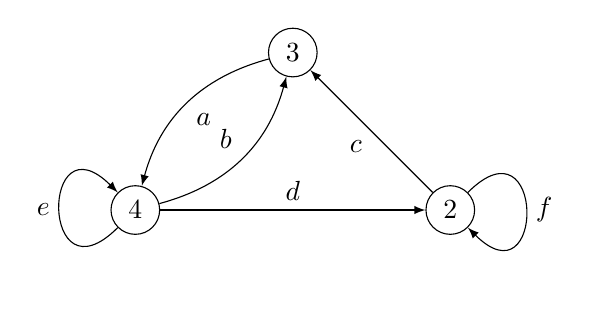
\begin{tikzpicture}
	\begin{pgfonlayer}{nodelayer}
		\node [style=state] (0) at (-2, -0) {$4$};
		\node [style=state] (1) at (2, -0) {$2$};
		\node [style=state] (2) at (0, 2) {$3$};
	\end{pgfonlayer}
	\begin{pgfonlayer}{edgelayer}
		\draw [style=transition, in=135, out=-135, loop] (0) to node[auto]{$e$} ();
		\draw [style=transition, in=-45, out=45, loop] (1) to node[auto]{$f$} ();
		\draw [style=transition] (0) to node[auto]{$d$} (1);
		\draw [style=transition] (1) to node[auto]{$c$} (2);
		\draw [style=transition, bend right, looseness=1.00] (2) to node[auto]{$a$} (0);
		\draw [style=transition, bend right, looseness=1.00] (0) to node[auto]{$b$} (2);
	\end{pgfonlayer}
\end{tikzpicture}
\end{center}

Additionally, let the following matrices be given:
\[
a' = \left( \begin{array}{cccc}
1 & 0 & 2 & 1 \\ 0 & 1 & 2 & 5 \\ 1 & 1 & 2 & 1
\end{array} \right)
\qquad 
b' = \left( \begin{array}{ccc}
1 & 0 & 1 \\ 0 & 1 & 1 \\ 2 & 2 & 2 \\ 1 & 5 & 1
\end{array} \right)
\qquad 
c' = \left( \begin{array}{ccc}
4 & 5 & 6 \\ 1 & 2 & 3
\end{array} \right)
\]

\[
d' = \left( \begin{array}{cc}
7 & 4 \\ 5 & 3 \\ 3 & 5 \\ 4 & 7
\end{array} \right)
\qquad
e' = \left( \begin{array}{cccc}
1&2&3&4 \\ 2&3&4&1 \\ 3&4&1&2 \\ 1&0&0&0
\end{array} \right)
\qquad
f' = \left( \begin{array}{cc}
1&2 \\ 2&0
\end{array} \right)
\]

We consider the categories $\pathcat{G}$, the path category of $G$, and
$\mathrm{MAT}(\mathbb{N})$, the category of matrices over $\mathbb{N}$.

Define
\[ \phi_1(i) = i\text{ for }i = 2, 3, 4 \]
and
\[ \phi'_2(x) = x'\text{ for }x \in \setof{a, b, c, d, e, f} \]

Then $\phi'_2$ can be extended in a unique way to a mapping $\phi_2 :
\pathcat{G} \to MAT(\mathbb{N})$ such that
\[ \phi = (\pathcat{G}, \mathrm{MAT}(\mathbb{N}), \phi_1, \phi_2) \]
is a functor.
\end{example}

\bigskip
We want to define now some special properties of functors.

\begin{definition}
Let $G_1, G_2$ be ordered graphs, $\phi = (\pathcat{G_1}, \pathcat{G_2},
\phi_1, \phi_2)$ a functor. $\phi$ is called {\bf ordered} or {\bf order
preserving} if it holds:

Let $\phi_1(v) = v' \in V_2$ for any $v \in V_1$, then for the ordering
\[ e_1, \ldots, e_k, e'_m, \ldots, e'_1 \]
which belongs to $v$ it holds:
\[ \phi_2(e_1), \ldots, \phi_2(e_k), \phi_2(e'_m), \ldots, \phi_2(e'_1) \]
is contained in the ordering that belongs to $v'$ in the given order. 
\end{definition}

It is possible that edges coincide which are counted only once in that case.

We explain this definition at the following example:

Let $v \in V_1$ be a point with ordering 
\[ s_1, s_2, s_3, s'_4, s'_3, s'_2, s'_1 \]
and $v' \in V_2$ be a point with ordering
\[ r_1, r_2, r'_5, r'_4, r'_3, r'_2, r'_1 \]
as shown in the following figure:

\begin{center}
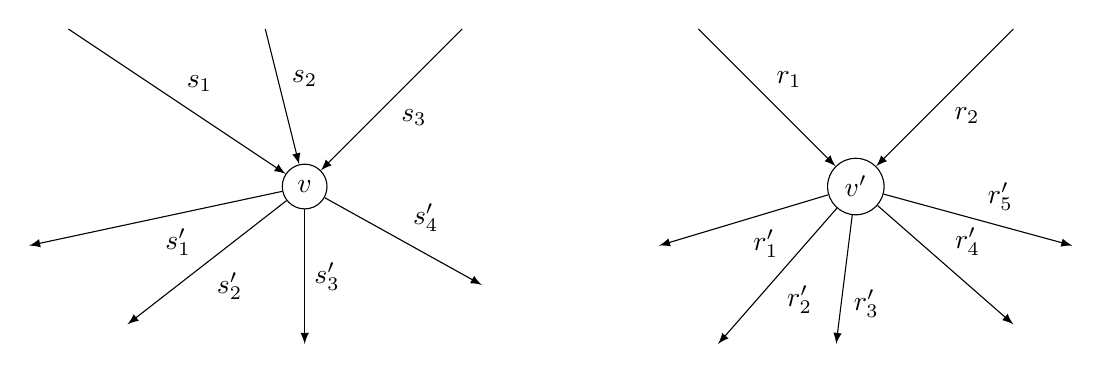
\begin{tikzpicture}
	\begin{pgfonlayer}{nodelayer}
		\node [style=state] (0) at (0, -0) {$v$};
		\node [style=state] (1) at (7, -0) {$v'$};
		\node [style=none] (2) at (-3, 2) {};
		\node [style=none] (3) at (-0.5, 2) {};
		\node [style=none] (4) at (2, 2) {};
		\node [style=none] (5) at (-3.5, -0.75) {};
		\node [style=none] (6) at (-2.25, -1.75) {};
		\node [style=none] (7) at (0, -2) {};
		\node [style=none] (8) at (2.25, -1.25) {};
		\node [style=none] (9) at (5, 2) {};
		\node [style=none] (10) at (9, 2) {};
		\node [style=none] (11) at (4.5, -0.75) {};
		\node [style=none] (12) at (5.25, -2) {};
		\node [style=none] (13) at (6.75, -2) {};
		\node [style=none] (14) at (9, -1.75) {};
		\node [style=none] (15) at (9.75, -0.75) {};
	\end{pgfonlayer}
	\begin{pgfonlayer}{edgelayer}
		\draw [style=transition] (2.center) to node[auto]{$s_1$} (0);
		\draw [style=transition] (3.center) to node[auto]{$s_2$} (0);
		\draw [style=transition] (4.center) to node[auto]{$s_3$} (0);
		\draw [style=transition] (0) to node[auto]{$s_1'$} (5.center);
		\draw [style=transition] (0) to node[auto]{$s_2'$} (6.center);
		\draw [style=transition] (0) to node[auto]{$s_3'$} (7.center);
		\draw [style=transition] (0) to node[auto]{$s_4'$} (8.center);
		\draw [style=transition] (9.center) to node[auto]{$r_1$} (1);
		\draw [style=transition] (10.center) to node[auto]{$r_2$} (1);
		\draw [style=transition] (1) to node[auto]{$r_1'$} (11.center);
		\draw [style=transition] (1) to node[auto]{$r_2'$} (12.center);
		\draw [style=transition] (1) to node[auto]{$r_3'$} (13.center);
		\draw [style=transition] (1) to node[auto]{$r_4'$} (14.center);
		\draw [style=transition] (1) to node[auto]{$r_5'$} (15.center);
	\end{pgfonlayer}
\end{tikzpicture}
\end{center}

Define $\phi$ by $\phi_1(v) = v'$ and
\begin{eqnarray*}
& \phi_2(s_1) = r_1,\ \phi_2(s_2) = r_2,\ \phi_2(s_3) = r_2 \\
& \phi_2(s'_1) = r'_1,\ \phi_2(s'_2) = r'_3,\ \phi_2(s'_3) = r'_4,\ \phi_2(s'_4)
= r'_5
\end{eqnarray*}
Then $\phi$ respects the ordering in point $v$.

\bigskip
\begin{definition}
Let $G_1=(V_1,E_1),\ G_2=(V_2,E_2)$ be oriented graphs and 
\[ \phi = (\pathcat{G_1}, \pathcat{G_2}, \phi_1, \phi_2)\text{ a functor.}
\]

$\phi$ is called {\bf regular} $\iff$ the restriction of $\phi_2$
to the set \[ \setof{e \in E_1 \mid Q(e) = v}\text{ and }\setof{e' \in E_2 \mid
Q(e') = \phi_1(v)} \] and to \[ \setof{e \in E_1 \mid Z(e) = v}\text{ and
}\setof{e' \in E_2 \mid Z(e') = \phi_1(v)} \] for $v \in V_1$ is bijective.
\end{definition}

To each incoming (outgoing) edge of a point $v \in V_1$ corresponds exactly
one incoming (outgoing) edge of $\phi_1(v) \in V_2$.

In our example, $\phi$ was not regular. We slightly weaken the definition of a
regular functor by postulating regularity only for the {\em outgoing} edges.

\bigskip
\begin{definition}
Let $G_1=(V_1,E_1),\ G_2=(V_2,E_2)$ be oriented graphs and
\[ \phi = (\pathcat{G_1}, \pathcat{G_2}, \phi_1, \phi_2)\text{ a functor.}
\]

$\phi$ is called {\bf out-regular} $\iff$ the restriction of $\phi_2$
to the set 
\[ \setof{e\in E_1 \mid Q(e) = v} \] and \[ \setof{e' \in E_2 \mid
Q(e') = \phi_1(v)} \]
for $v \in V_1$ is bijective.
\end{definition}

The following lemma holds (exercise):

\begin{lemma}
If $\phi = (\pathcat{G_1}, \pathcat{G_2}, \phi_1, \phi_2)$ is an out-regular
functor, then \\ $\phi(\pathcat{G_1})$ is a category.
\end{lemma}

Our next lemma describes a well-known fact from graph theory that has found many
applications.

\begin{lemma}
To each circle-free star $G = (V, E)$ relative to a point $c \in V$ there exists
a tree $B$ and an out-regular functor $(\pathcat{B}, \pathcat{G},
\phi_1, \phi_2)$ mapping the root of the tree $B$ to the point $c$. $B$ is 
uniquely determined up to isomorphisms.
\end{lemma}

\begin{proof}
Exercise.
\end{proof}



\section{Subcategory, generating system}

\begin{definition}
Let \[ U = (Obj(U), Mor(U), Q_U, Z_U, \circ_U) \] and \[C = (Obj(C), Mor(C),
Q_C, Z_C, \circ_C)\] be categories.

$U$ is called a {\bf subcategory} of $C \iff$
\begin{enumerate}
  \item $Obj(U) \subset Obj(C)$ and $Mor(U) \subset Mor(C)$
  \item $Q_U = Q_C|_{Mor(U)}$ and $Z_U = Z_C|_{Mor(U)}$
  \item $\circ_U = \circ_C|_{Mor(U) \times Mor(U)}$
  \item $w \in Obj(U) \Rightarrow 1_w \in Mor(U)$
\end{enumerate}
\end{definition}

$U$ is called {\bf full subcategory} of $C \iff$
\[ \forall w_1, w_2 \in Obj(U),\ f: w_1 \to w_2 \in Mor(C) \Rightarrow f \in
Mor(U) \]

In a full subcategory, all morphisms of $C$ between objects in $U$ are also
morphisms in $U$. $f: w_1 \to w_2$ stands for $Q(f) = w_1 \wedge Z(f) = w_2$.

We want to explain this fact at some examples:

\bigskip
{\bf Example 1}:

Let $A = \setof{x,y,z,a,b,c}$ and $f, g, h: A^* \to A^*$ be mappings defined
as follows:
\[ f(u_1 \cdot x \cdot u_2 \cdot x \cdots x \cdot u_k \cdot x) = 
u_1 \cdot ax \cdot u_2 \cdot ax \cdots ax \cdot u_k \cdot ax \]
where $u_i \in (A \setminus \setof{x})^*$,
\[ g(u_1 \cdot y \cdot u_2 \cdot y \cdots y \cdot u_k \cdot y) = 
u_1 \cdot by \cdot u_2 \cdot by \cdots by \cdot u_k \cdot by \]
where $u_i \in (A \setminus \setof{y})^*$,
\[ h(u_1 \cdot z \cdot u_2 \cdot z \cdots z \cdot u_k \cdot z = 
u_1 \cdot cz \cdot u_2 \cdot cz \cdots cz \cdot u_k \cdot cz) \]
where $u_i \in (A \setminus \setof{z})^*$.

Let $M$ be the monoid of mappings $m: A^* \to A^*$ generated by $f, g$ and $h$.
Then $C = (\setof{A^*}, M, Q, Z, \circ)$ is a category, if $\circ$ denotes the
monoid operation in $M$.

Let $G$ be the graph defined by the following figure:

\begin{center}
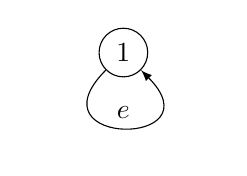
\begin{tikzpicture}
	\begin{pgfonlayer}{nodelayer}
		\node [style=state] (0) at (0, -0) {$1$};
	\end{pgfonlayer}
	\begin{pgfonlayer}{edgelayer}
		\draw [style=transition, in=-45, out=-135, loop] (0) to node[auto]{$e$} ();
	\end{pgfonlayer}
\end{tikzpicture}
\end{center}

We define a functor $\phi = (\pathcat{G}, C, \phi_1, \phi_2)$ by
\begin{eqnarray*}
\phi_1(1) & := & A^* \\
\phi_2(e) & := & f \circ g \circ h
\end{eqnarray*}

$\phi_2(\pathcat{G})$ is a subcategory of $C$ (exercise) and it holds:
\[ \phi_2(\pathcat{G})(xyz) = \setof{a^n x b^n y c^n z \mid n \in \mathbb{N}}
\]

\bigskip
{\bf Example 2}:

We continue with example 1. In addition to $f,g,h$ we add three monoid
homomorphisms $f_1, g_1, h_1$ defined by:
\[\begin{array}{l@{,\quad}l@{\quad}l}
f_1(x) = \epsilon & f_1(u) = u & \forall u \in A \setminus \setof{x} \\
g_1(y) = \epsilon & g_1(u) = u & \forall u \in A \setminus \setof{y} \\
h_1(z) = \epsilon & h_1(u) = u & \forall u \in A \setminus \setof{z}
\end{array}\]

We extend the graph $G$ as follows to a graph $G_1$:

\begin{center}
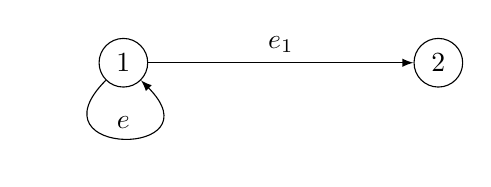
\begin{tikzpicture}
	\begin{pgfonlayer}{nodelayer}
		\node [style=state] (0) at (0, -0) {$1$};
		\node [style=state] (1) at (4, -0) {$2$};
	\end{pgfonlayer}
	\begin{pgfonlayer}{edgelayer}
		\draw [style=transition, in=-45, out=-135, loop] (0) to node[auto]{$e$} ();
		\draw [style=transition] (0) to node[auto]{$e_1$} (1);
	\end{pgfonlayer}
\end{tikzpicture}
\end{center}

Consider $\pathcat{G_1}(1,2)$. Then $\pathcat{G_1}(1,2) \cup \setof{1_1,
1_2}$ is a subcategory of $\pathcat{G_1}$. In addition, $\pathcat{G}$ is a subcategory of
$\pathcat{G_1}$.

We extend the functor $\phi$ from example 1 onto $\pathcat{G_1}$ by defining:
\[ \phi_2(e_1) := f_1 \circ g_1 \circ h_1 \]

We get:
\[ \phi_2(\pathcat{G_1}(1,2))(xyz) = \setof{a^n b^n c^n \mid n \in \mathbb{N}}
\]

\bigskip
{\bf Example 3}:

Let $G$ be defined as follows:

\begin{center}
\begin{tikzpicture}
	\begin{pgfonlayer}{nodelayer}
		\node [style=state] (0) at (0, 6) {$1$};
		\node [style=state] (1) at (-3, 4) {$6$};
		\node [style=state] (2) at (3, 4) {$2$};
		\node [style=state] (3) at (-3, -0) {$5$};
		\node [style=state] (4) at (3, -0) {$3$};
		\node [style=state] (5) at (0, -2) {$4$};
		\node [style=state] (6) at (7, 2) {$2'$};
		\node [style=state] (7) at (9, 4) {$1'$};
		\node [style=state] (8) at (9, -0) {$3'$};
	\end{pgfonlayer}
	\begin{pgfonlayer}{edgelayer}
		\draw [style=transition] (0) to (2);
		\draw [style=transition] (2) to (4);
		\draw [style=transition] (4) to (5);
		\draw [style=transition] (5) to (3);
		\draw [style=transition] (3) to (1);
		\draw [style=transition] (1) to (0);
		\draw [style=transition] (2) to (6);
		\draw [style=transition] (4) to (8);
		\draw [style=transition] (7) to (6);
		\draw [style=transition] (6) to (8);
		\draw [style=transition] (8) to (7);
		\draw [style=transition] (1) to (8);
		\draw [style=transition] (3) to (6);
		\draw [style=transition] (0) to (7);
		\draw [style=transition, bend right=75, looseness=1.75] (5) to (7);
	\end{pgfonlayer}
\end{tikzpicture}
\end{center}

The full subcategory of $\pathcat{G}$ generated by $\setof{1', 2', 3'}$ is the
path category $\pathcat{G'}$ with the following graph $G'$:

\begin{center}
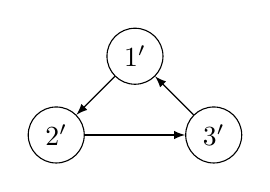
\begin{tikzpicture}
	\begin{pgfonlayer}{nodelayer}
		\node [style=state] (0) at (0, 1) {$1'$};
		\node [style=state] (1) at (-1, -0) {$2'$};
		\node [style=state] (2) at (1, -0) {$3'$};
	\end{pgfonlayer}
	\begin{pgfonlayer}{edgelayer}
		\draw [style=transition] (0) to (1);
		\draw [style=transition] (1) to (2);
		\draw [style=transition] (2) to (0);
	\end{pgfonlayer}
\end{tikzpicture}
\end{center}

One can show (exercise): The mapping $\phi_1$ defined by 
\[ \phi_1(1) = 1' \quad \phi_1(4) = 1' \quad \phi_1(2) = 2' \quad \phi_1(5) = 2'
 \quad \phi_1(3) = 3' \quad \phi_1(6) = 3' \]
can be extended to a functor $\phi = (\pathcat{G}, \pathcat{G'}, \phi_1,
\phi_2)$ by defining $\phi_2$ in a suitable way.

Remark: The preimage of a closed path does not have to be closed.

We prove now the following
\begin{lemma}
Let \[ C_i = (O_i, M_i, Q, Z, \circ),\ i = 1, 2, 3 \] be categories and $C_1$
and $C_2$ be subcategories of $C_3$. Then $C_1 \cap C_2$ is a category.
\end{lemma}

\begin{proof}
It holds
\begin{enumerate}
  \item $w \in O_1 \cap O_2 \Rightarrow 1_w \in M_1 \cap M_2$
  \item $f, g \in M_1 \cap M_2 \Rightarrow f \circ g \in M_1 \cap M_2$, if
  $Z(f) = Q(g)$
\end{enumerate}
It follows that $C_1 \cap C_2$ is a category.
\end{proof}

\bigskip
\begin{lemma}
Let $ C_i = (O_i, M_i, Q, Z, \circ),\ i \in I,$\ where $I$ is an arbitrary
index set, be categories. If $C_i,\ i \in I,$ are subcategories of a category
$C$, then 
\[ \tilde{C} := \bigcap_{i \in I} C_i \] 
is a category.
\end{lemma}
The proof is similar as the one of the previous lemma.

\bigskip
\begin{definition}
Let $C = (O, M, Q, Z, \circ)$\ be a category and $O_1 \subset O,\ M_1 \subset M$
and 
\[ \category{U}_C(O_1, M_1) := \setof{C' \mid C'\text{ is subcategory of }C,\
O_1 \subset O',\ M_1 \subset M'} \]
Then 
\[ \generatedby{O_1}{M_1} := \bigcap_{C' \in \category{U}_C(O_1, M_1)} C' \]
is called the {\bf subcategory} of $C$ generated by the {\bf generating system}
$(O_1, M_1)$.
\end{definition}

Obviously for each category $C = (O, M, Q, Z, \circ)$ it holds $C =
\generatedby{O}{M}$.

We say $M_1$ {\bf generates} \generatedby{O_1}{M_1} if 
\[ O_1 = \setof{Q(m) \mid m \in M_1} \cup \setof{Z(M) \mid m \in M_1} \]

We have already seen an example for a nontrivial generating system.

Let $G=(V,E)$ be a graph, then $E$ is a generating system of $\pathcat{G}$
which means $\pathcat{G} = \generatedbyone{E(G)}$. The path category of a graph
has a special property namely that $E(G)$ is a {\bf free generating system} of
$\pathcat{G}$.

\bigskip
\begin{definition}
Let $C = (O, M, Q, Z, \circ)$ be a category and $E \subset M$. $E$ is called a
{\bf free generating system} of $C$ if the following holds:

If $C' = (O', M', Q, Z, \circ)$ is an arbitrary category and $\phi_1 : O \to O'$
and $\phi_s : E \to M'$ are mappings which make the following diagram commute:

\begin{center}
\begin{tikzcd}[row sep=large,column sep=huge]
 O \arrow[leftarrow]{r}{Q} \arrow{d}{\phi_1} & E \arrow{r}{Z}
 \arrow{d}{\phi'_2} & O \arrow{d}{\phi_1} \\
 O' \arrow[leftarrow]{r}{Q} & M' \arrow{r}{Z} & O'
\end{tikzcd}
\end{center}

Then there exists a unique continuation of $\phi'_2$ to $\phi_2 : M \to M'$ such
that $\phi = (C, C', \phi_1, \phi_2)$ is a functor.
\end{definition}

\begin{definition}
A category $C$ is called {\bf free} if there exists a free generating system $E$
of $C$.
\end{definition}

We formulate now our observation above as a theorem:

\begin{theorem}
Let $G=(V, E)$ be a graph. Then $E$ is a free generating system of
$\pathcat{G}$.
\end{theorem}

\transrem{In the following proof some variable names have been changed to avoid
confusion}

\begin{proof}
Let $G = (V, E)$ be a graph and $C$ an arbitrary category, let $\phi_1 :
E \to O,\ \phi'_2 : E \to M$ be mappings and the following diagram commute:

\begin{center}
\begin{tikzcd}[column sep=huge,row sep=large]
 V \arrow[leftarrow]{r}{Q} \arrow{d}{\phi_1} & E \arrow{r}{Z}
 \arrow{d}{\phi'_2} & V \arrow{d}{\phi_1} \\
 O \arrow[leftarrow]{r}{Q} & M \arrow{r}{Z} & O
\end{tikzcd}
\end{center}

We define 
\[ \phi_2(v,v) = 1_{\phi_1(v)},\ v \in V \] 
and 
\[ \phi_2(e) = \phi'_2(e),\ e \in E \]

Let $\phi_2(\pi)$ be defined for all paths $\pi \in \pathcat{G}$ with $|\pi|
\leq n,\ n \geq 1$ and $\phi_2$ be compatible with $Q$ and $Z$ for all these
paths $\pi$.

Further let $\phi_2$ be uniquely determined for these paths $\pi$ and it holds:
\[ \phi_2(\pi \cdot \psi) = \phi_2(\pi) \cdot \phi_2(\psi) \]
for all $\pi, \psi$ with $|\pi \cdot \psi| \leq n$.

Now let $\omega = (v, e_1, \ldots, e_{n+1}, v') \in \pathcat{G}$. We split
$\omega$ into 
\[ \omega = (v, \underbrace{e_1, \ldots, e_n}_{\omega_1}, v'') \cdot (v'',
\underbrace{e_{n+1}}_{\omega_2}, v')
\]
By induction hypothesis, $\phi_2(\omega_1)$ and $\phi_2(\omega_2)$ are defined.

For $\phi_2$ to become a functor, necessarily $\phi_2(\omega) = \phi_2(\omega_1)
\cdot \phi_2(\omega_2)$ must hold.

By assumption, $\phi_2$ is compatible with source and target mappings $Q$ and
$Z$ for $\omega_1$ and $\omega_2$. Therefore $Z(\phi_2(\omega_1)) =
Q(\phi_2(\omega_2))$ and $\phi_2(\omega)$ are defined.

Let $\omega = \psi_1 \cdot \psi_2$ be any partition of $\omega$, so 
\[ \omega = (v, \underbrace{e_1, \ldots, e_j}_{\psi_1}, \bar{v}) \cdot (\bar{v},
\underbrace{e_{j+1}, \ldots, e_{n+1}}_{\psi_2}, v') \]

By induction hypothesis it holds:
\begin{enumerate}
  \item $Z(\phi_2(\psi_1)) = Q(\phi_2(\psi_2))$, so $\phi_2(\psi_1) \cdot
  \phi_2(\psi_2)$ is defined.
  \item With $\psi'_2 = (\bar{v}, e_{j+1}, \ldots, e_n, v'')$ we have
  \begin{eqnarray*}
  \phi_2(\psi_1) \cdot \phi_2(\psi_2) & = & \phi_2(\psi_1) \cdot
  (\phi_2(\psi'_2) \cdot \phi_2(\psi_2)) \\
  & = & (\phi_2(\psi_1) \cdot \phi_2(\psi'_2)) \cdot \phi_2(\omega_2) \\
  & = & \phi_2(\omega_1) \cdot \phi_2(\omega_2) \\
  & = & \phi_2(\omega)
  \end{eqnarray*}
\end{enumerate}

It remains to show 
\[ \phi_1(Q(\omega)) = Q(\phi_2(\omega)),\quad \phi_1(Z(\omega)) =
Z(\phi_2(\omega)) \]

This follows directly from $Q(\omega) = Q(\omega_1)$ and $Z(\omega) =
Z(\omega_2)$ by application of the induction hypothesis.
\end{proof}

\bigskip
\begin{theorem}
To each category $C$ there exists a free category $F$ and a surjective functor
$\phi = (F, C, \phi_1, \phi_2)$.
\end{theorem}

\begin{proof}
For the category $C$ we create an oriented graph $G_C = (V, E)$ with 
\begin{eqnarray*}
V &=& Obj(C) \\
E &=& \setof{f \mid Q(f) = O_1,\ Z(f) = O_2,\ f : O_1 \to O_2 \in M}
\end{eqnarray*}
i.e\ the objects of the category become the points (vertices) of the graph and
each morphism becomes an edge. Because $\pathcat{G_C}$ is a free category by
theorem 1, we can choose $F$ to be exactly this category.

Let $\phi_1 : V \to O$ with $\phi_1(w) = w$ and $\phi'_2 : E \to M$ with
$\phi'_2(f) = f$ be mappings and $\phi_2 : \pathcat{G_C} \to M$ be the
continuation of $\phi'_2$ such that $\phi = (\pathcat{G_C}, C, \phi_1, \phi_2)$
becomes a functor.

By construction, $\phi$ is surjective.
\end{proof}

\bigskip
The following theorem tells about the uniqueness of free generating systems.
\begin{theorem}
If $E$ and $E'$ are free generating systems of a category $F$, then $E = E'$.
\end{theorem}

The proof is similar to prrof of the corresponding theorem for free monoids.

\section{Grammars and derivations}

In the introduction to this book we already learned about examples of formal
languages. The wish to describe these in general infinite sets of words by a
finite generating system leads to the notion of a {\bf grammar}.

\begin{definition}
$G = (N, T, P, S)$ is a {\bf (Chomsky-) grammar}, if
\begin{enumerate}
  \item $N$ is a finite non-empty set of {\bf nonterminal symbols}
  \item $T$ is a finite non-empty set of {\bf terminal symbols} with
  $N \cap T = \emptyset$
  \item $P \subset N^+ \times (N \cup T)^*$ is a finite set of {\bf productions}
  \item $S \in N$ is the {\bf axiom} or {\bf start symbol} 
\end{enumerate}
\end{definition}

Notation: For $p = (u, v) \in P$ we also write $u \production{p} v$ and
$Q(p) = u,\ Z(p) = v$ ({\em source} and {\em target} of a production).

Examples:
\begin{enumerate}
  \item $G_1 = (N, T, P, S)$ with $N = \setof{S},\ T = \setof{x, x'},$ \\ 
  $P = \setof{S \to SS,\ S \to xSx',\ S \to \epsilon}$
  \item $G_2 = (N, T, P, S)$ with $N = \setof{S, X},\ T = \setof{x, x'}$ \\
  $P = \setof{S \to xSX,\ S \to xX, X \to x'S,\ X \to x'}$
\end{enumerate}

To generate the words of a language using a grammar, starting with the axiom
intermediate words are generated by multiple application of productions
until the produced word contains terminal symbols only. This leads to the
notion of a {\em derivation} that will now be formally defined.

\begin{definition}
Let $G = (N, T, P, S)$ be a grammar and $w, w' \in (N \cup T)^*$.

$w'$ is {\bf directly derivable} from $w$ using $G$ ($w \dderives{G} w'$) if
there are decompositions 
\[ w = w_1 \cdot u \cdot w_2\text{ and }w' = w_1 \cdot v \cdot w_1 \]
and there is a production $(u, v) \in P$.

$w'$ is {\bf derivable} from $w$ ($w \derives{G} w'$) if there exists
a sequence of words 
\[ w = w_0, \ldots, w_n = w',\quad n \in \mathbb{N},\ w_i \in (N \cup T)^* \]
such that $w_i \dderives{G} w_{i+1},\ 0 \leq i \leq n$.
\end{definition}

Such a sequence is called a {\bf derivation} of length $n$. $Q$ and $Z$ can be
extended in a natural way to derivations.

A derivation is called {\bf canonic} or {\bf leftmost} if in each step $w
\dderives{G} w'$ the following holds:

If $w = w_1 \cdot u \cdot w_2$ and $w' = w_1 \cdot v \cdot w_2$ are the
decompositions and $(u, v) \in P$ is the applied production, then $w_1 \in T^*$.
This means that always the leftmost nonterminal is replaced.

If the grammar is known, we omit $G$ from the relation
symbols $\dderives{G}$ and $\derives{G}$. 

We consider some properties of the relation $\derives{G}$:

\begin{lemma}
Let $G$ be a grammar. It holds:
\begin{enumerate}
  \item $(u, v) \in P \ \Rightarrow\ u \derives{G} v$
  \item $w \derives{G} w$ (reflexivity)
  \item $w \derives{G} w' \wedge w' \derives{G} w'' \ \Rightarrow\ w \derives{G}
  w''$ (transitivity)
  \item $w_1 \derives{G} w'_1 \wedge w_2 \derives{G} w'_2\ \Rightarrow\ w_1
  \cdot w_2 \derives{G} w'_1 \cdot w'_2$ (compatibility with monoid operation)
\end{enumerate}
Here, $w, w', w'', w_1, w_2, w'_1, w'_2 \in (N \cup T)^*$.
\end{lemma}

\begin{proof}\ 

\begin{enumerate}
  \item follows from the definition of $\derives{G}$.
  \item clear with $n = 0$ in the definition of $\derives{G}$.
  \item There exist sequences $w = w_0, \ldots, w_n = w',\ w' = w'_0, \ldots,
  w'_m = w''$ with $w_i \derives{G} w_{i+1}$ and $w'_j \derives{G} w'_{j+1}$.
  Because $w_n = w' = w'_0$, the composed sequence $w = w_0, \cdots, w_n, w'_1,
  \cdots, w'_n = w''$ is a derivation from $w$ to $w''$.
  \item Exercise for the reader
\end{enumerate}
\end{proof}

Notation: An intermediate word that is generated by a derivation starting with
the axiom is called a {\bf sentence form} of $G$. We define:

\begin{definition}
\[ \mathrm{SF}(G) := \setof{w \in (N \cup T)^* \mid S \derives{G} w} \]
is the set of {\bf sentence forms} of $G$.
\end{definition}

Now we are able to define the formal language generated by a grammar.

\begin{definition}
Let $G = (N, T, P, S)$ be a grammar.
\[ L(G) := \setof{w \in T^* \mid S \derives{G} w} \]
is the {\bf language generated by} $G$.
\end{definition}

Note: $L(G) = \mathrm{SF}(G) \cap T^*$.

Examples:
\begin{enumerate}
  \item One can see that for the grammar $G_1$ from example 1 it holds: $L(G_1)$
  is the Dyck language over the alphabet $\setof{x, x'}$.
  \item Let $G = (N, T, P, S)$ with $N = \setof{S},\ T = \setof{a, b},\\
  P = \setof{S \to aSb, S \to \epsilon}$.\\
  Then $L(G) = \setof{a^n b^n \mid n \in \mathbb{N}}$. The simple proof is left
  to the reader.
\end{enumerate}

Grammars are compared with respect to the languages they generate. We define:

\begin{definition}
$G$ is {\bf (weakly) equivalent} to $G' \iff L(G) = L(G')$.
\end{definition}

Remark: The reader should convince himself that the grammars $G_1$ and $G_2$
from the first example generate the same language.

Of course you can define infinitely many different grammars for each language.

We can define now different classes of grammars (and languages generated by
them) depending on certain restrictions of their production systems. In the next
chapter we will meet the so called {\em right-linear} grammars and their
languages.

Of special importance, also from a practical point of view, are the so
called {\em context-free} grammars.

\begin{definition}
A grammar $G = (N, T, P, S)$ is called {\bf context-free} $\iff P \subset N
\times (N \cup T)^*$.
\end{definition}

The term {\em context-free} describes the fact that in a sentence-form a
nonterminal symbol may be replaced by the right-hand side of a production
without having to take the ''context'' of that symbol, i.e.\ the symbols to the
left or right, into account.

In chapter 4 we will treat context-free grammars in depth.

\chapter{Finite Automata}
\section{The finite automaton, regular sets in $X^*$,\ $\reglang(X^*)$}

Let $G = (V, E)$ be a finite, oriented graph, $X$ a finite set and $\alpha =
(\pathcat{G}, X^*,\alpha_1, \alpha_2)$ a functor with $\alpha_1 : V \to
\setof{X^*},\ \alpha_2 : \pathcat{G} \to X^*$.

\begin{definition}
$\fa{A} = (G, X^*, \alpha)$ is called a {\bf nondeterministic finite
automaton}.
\end{definition}

\transrem{Here the free monoid $X^*$ is regarded as a category
$X^* = (\setof{X^*}, X^*, Q, Z, \cdot \})$ where $\cdot$ is the monoid
operation (word concatenation). Words are treated as morphisms with source and target
$X^*$.}

If $S, F \subset V$, we call 
\[ \fa{A} = (G, X^*, s, f, \alpha) \]
a finite automaton with start and final states or shortly a {\bf finite
acceptor}.

In the following we will use the terms {\em acceptor} and {\em finite automaton}
as synonyms.

If the finite automaton works over the free monoid $X^*$ we write shorter just
$X$ instead of $X^*$, otherwise we specify the monoid explicitly.

If we define 
\[ \pathcat{G}(S, F) := \setof{\pi \in \pathcat{G} \mid Q(\pi) \in S,\ Z(\pi)
\in F}
\] 
then $L_{\fa{A}} := \alpha_2(\pathcat{G}(S, F))$ is called the {\bf set accepted
by} \fa{A}.

We will also write shortly $\alpha$ instead of $\alpha_2$ and $\pathcat{}(S,F)$
instead of $\pathcat{G}(S,F)$.

\begin{definition}
Let $X$ be an alphabet. 
\[ \reglang(X^*) := \setof{L \subset X^* \mid \mbox{ there exists a finite acceptor
}\fa{A} \mbox{ with } L = L_{\fa{A}}} \]

$\reglang(X^*)$ is called the {\bf set of regular languages} over the free monoid
$X^*$.
\end{definition}

Remark: We defined the finite automaton via its ''state graph''. Most
often, the definition is given using the ''next state relation'' as follows:
\begin{eqnarray*}
\delta &=& \{(a, v_1, v_2) \in X \times V \times V) \mid \\
&& \mbox{there exists an edge } e \mbox{ with } Q(e) = v_1,\ Z(e) = v_2 \mbox{
and } \alpha(e) = a \in X \}
\end{eqnarray*}

$\delta$ my be regarded as a relation between $X \times V$ and $V$ where $X$ is
the input alphabet and $V$ the state set of the automaton \[ \fa{B} = (X,
V, \delta, S, F) \]

The elements of $V$ denote the current state of the automaton $\fa{B}$.

If the automaton $\fa{B}$ is in state $v \in V$ and reads the symbol $x
\in X$ then it changes into state $v' \in V$ where $(x, v, v') \in \delta$. If
there doesn't exist such a $v'$ the automaton halts.

This interpretation can be visualized as follows:

\missingfigure

Let's return to our definition of the finite automaton. We explain its
working based on our definition:

The automaton $\fa{A} = (G, X, S, F, \alpha)$ may be interpreted as a
nondeterministic algorithm. The points (vertices) of the graph $G$ define the
possible states of the algorithm, the elements of $X$ are the input alphabet.

The nondeterministic automaton $\fa{A}$ which reads a symbol $x \in X$
while in state $v \in V$ changes into state $v'$ if there exists an edge $e$
from $v$ to $v'$ with label $\alpha(e) = x$. If the graph has no such edge
originating in $v$ the automaton is set ''out of service''.

A finite acceptor accepts a word $w \in X^*$ if there exists a path from a point
in $S$ to a point in $F$ which is labelled with the word $w$.

Let's consider some examples for finite automata:

\begin{example}
Let $X = \setof{a, b}$ and $L = \setof{(a b)^{2n} \mid n \in
\mathbb{N}}$.

It holds: $L \in \reglang(\setof{a, b}^*)$.

The acceptor $\fa{A} = (G, \setof{a, b}, {1}, {1}, \alpha)$ accepts $L$
(exercise):
\begin{center}
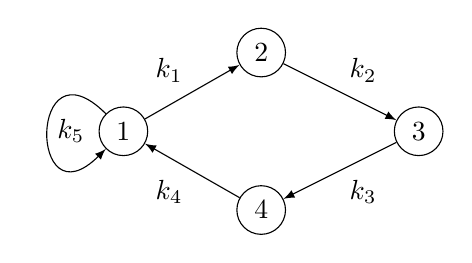
\begin{tikzpicture}
	\begin{pgfonlayer}{nodelayer}
		\node [style=state] (0) at (-1.75, -0) {$1$};
		\node [style=state] (1) at (2, -0) {$3$};
		\node [style=state] (2) at (0, 1) {$2$};
		\node [style=state] (3) at (0, -1) {$4$};
	\end{pgfonlayer}
	\begin{pgfonlayer}{edgelayer}
		\draw [style=transition] (0) to node[auto]{$k_1$} (2);
		\draw [style=transition] (2) to node[auto]{$k_2$} (1);
		\draw [style=transition] (1) to node[auto]{$k_3$} (3);
		\draw [style=transition] (3) to node[auto]{$k_4$} (0);
		\draw [style=transition, in=-135, out=135, loop] (0) to node[auto]{$k_5$} ();
	\end{pgfonlayer}
\end{tikzpicture}
\end{center}
\end{example}

\bigskip
Example 2: Lexical analysis, check for special characters.

In every programming language there exist special character combinations
(reserved words) that mark certain program actions. These have to be identified
during the lexical analysis. We give a finite acceptor which realizes such a check for a selection
of reserved words:

Let the set of reserved words be 
\begin{center}
\{\,'BEGIN',\ 'END',\ 'ELSE',\ 'IF',\ FI',\ 'FOR',\ 'INTEGER',\ 'THEN',\
'LOOP',\ 'POOL',\ 'PROCEDURE'\,\}
\end{center}

The following acceptor accepts this set:

\begin{minipage}{\textwidth}
\begin{sideways}
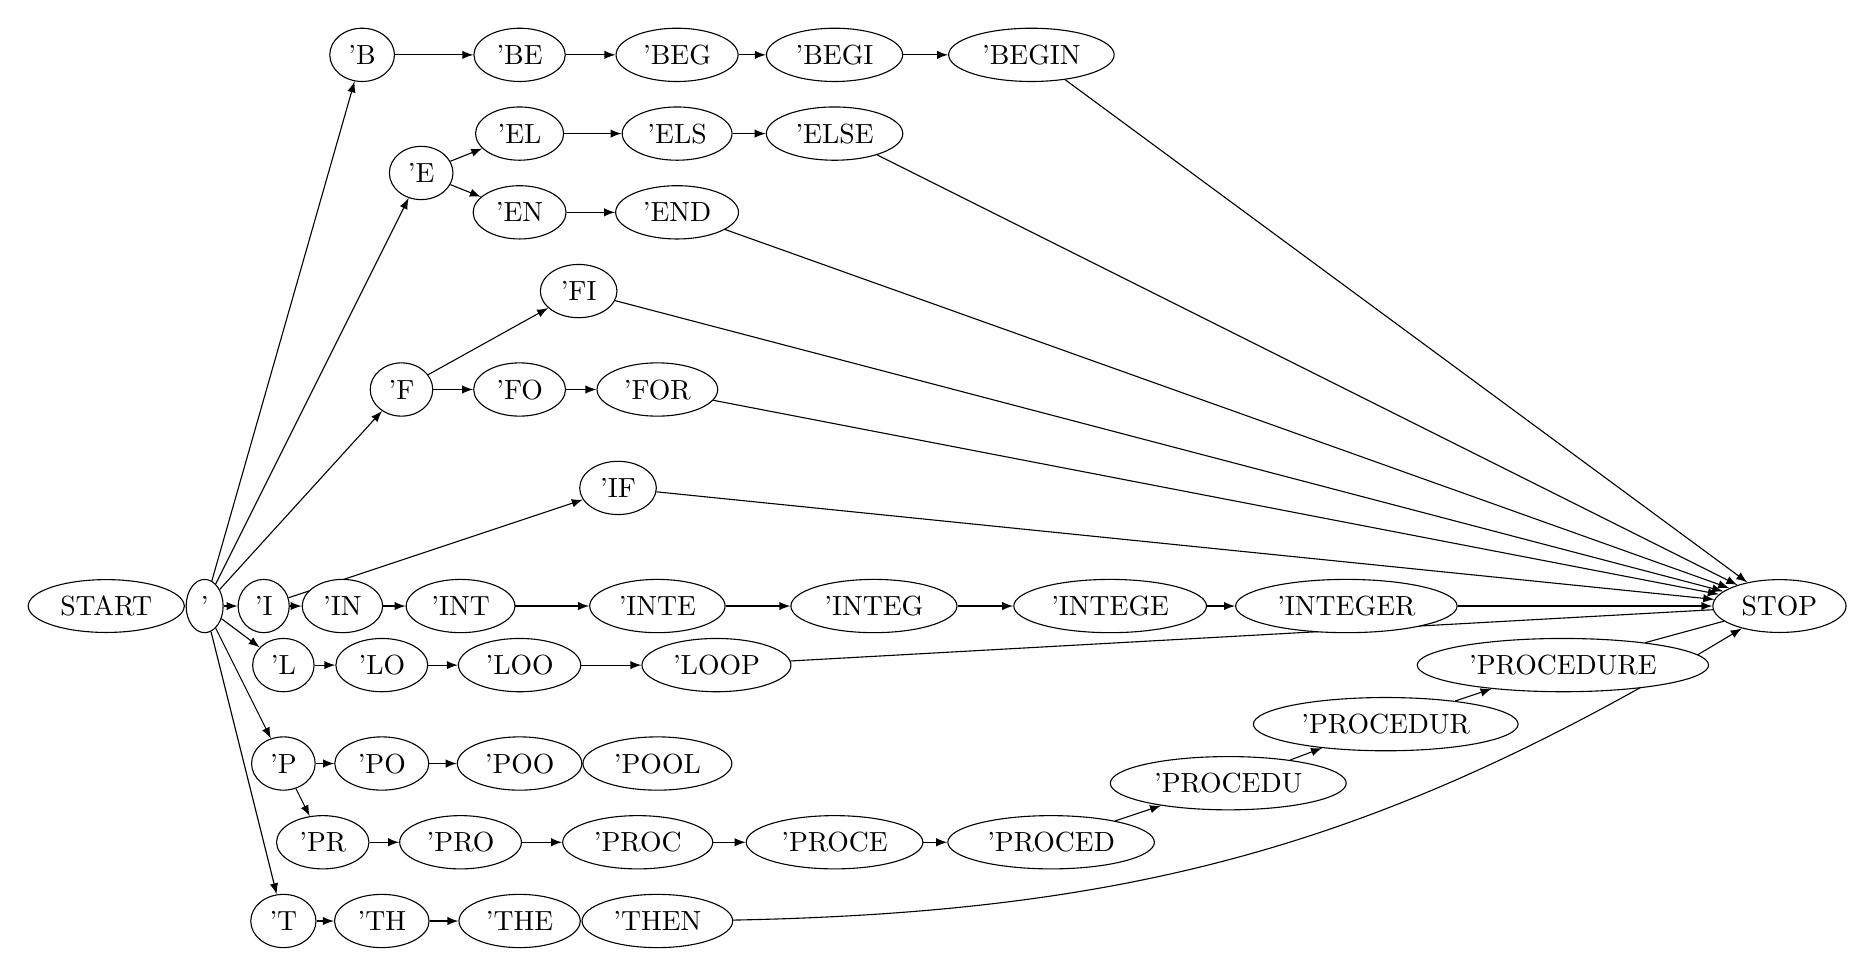
\begin{tikzpicture}
	\begin{pgfonlayer}{nodelayer}
		\node [style={oval_state}] (0) at (-14.25, -0) {START};
		\node [style={oval_state}] (1) at (-13, -0) {'};
		\node [style={oval_state}] (2) at (-12.25, -0) {'I};
		\node [style={oval_state}] (3) at (-7.75, 1.5) {'IF};
		\node [style={oval_state}] (4) at (-11.25, -0) {'IN};
		\node [style={oval_state}] (5) at (-9.75, -0) {'INT};
		\node [style={oval_state}] (6) at (-7.25, -0) {'INTE};
		\node [style={oval_state}] (7) at (-4.5, -0) {'INTEG};
		\node [style={oval_state}] (8) at (-1.5, -0) {'INTEGE};
		\node [style={oval_state}] (9) at (1.5, -0) {'INTEGER};
		\node [style={oval_state}] (10) at (7, -0) {STOP};
		\node [style={oval_state}] (11) at (-10.5, 2.75) {'F};
		\node [style={oval_state}] (12) at (-8.25, 4) {'FI};
		\node [style={oval_state}] (13) at (-9, 2.75) {'FO};
		\node [style={oval_state}] (14) at (-7, 6) {'ELS};
		\node [style={oval_state}] (15) at (-7.25, 2.75) {'FOR};
		\node [style={oval_state}] (16) at (-10.25, 5.5) {'E};
		\node [style={oval_state}] (17) at (-9, 6) {'EL};
		\node [style={oval_state}] (18) at (-5, 6) {'ELSE};
		\node [style={oval_state}] (19) at (-9, 5) {'EN};
		\node [style={oval_state}] (20) at (-7, 5) {'END};
		\node [style={oval_state}] (21) at (-11, 7) {'B};
		\node [style={oval_state}] (22) at (-9, 7) {'BE};
		\node [style={oval_state}] (23) at (-7, 7) {'BEG};
		\node [style={oval_state}] (24) at (-5, 7) {'BEGI};
		\node [style={oval_state}] (25) at (-2.5, 7) {'BEGIN};
		\node [style={oval_state}] (26) at (-12, -0.75) {'L};
		\node [style={oval_state}] (27) at (-10.75, -0.75) {'LO};
		\node [style={oval_state}] (28) at (-9, -0.75) {'LOO};
		\node [style={oval_state}] (29) at (-6.5, -0.75) {'LOOP};
		\node [style={oval_state}] (30) at (-12, -2) {'P};
		\node [style={oval_state}] (31) at (-10.75, -2) {'PO};
		\node [style={oval_state}] (32) at (-9, -2) {'POO};
		\node [style={oval_state}] (33) at (-7.25, -2) {'POOL};
		\node [style={oval_state}] (34) at (-11.5, -3) {'PR};
		\node [style={oval_state}] (35) at (-9.75, -3) {'PRO};
		\node [style={oval_state}] (36) at (-7.5, -3) {'PROC};
		\node [style={oval_state}] (37) at (-5, -3) {'PROCE};
		\node [style={oval_state}] (38) at (-2.25, -3) {'PROCED};
		\node [style={oval_state}] (39) at (0, -2.25) {'PROCEDU};
		\node [style={oval_state}] (40) at (2, -1.5) {'PROCEDUR};
		\node [style={oval_state}] (41) at (4.25, -0.75) {'PROCEDURE};
		\node [style={oval_state}] (42) at (-12, -4) {'T};
		\node [style={oval_state}] (43) at (-10.75, -4) {'TH};
		\node [style={oval_state}] (44) at (-9, -4) {'THE};
		\node [style={oval_state}] (45) at (-7.25, -4) {'THEN};
	\end{pgfonlayer}
	\begin{pgfonlayer}{edgelayer}
		\draw [style=transition] (1) to (2);
		\draw [style=transition] (2) to (3);
		\draw [style=transition] (2) to (4);
		\draw [style=transition] (4) to (5);
		\draw [style=transition] (5) to (6);
		\draw [style=transition] (6) to (7);
		\draw [style=transition, in=180, out=0, looseness=1.00] (7) to (8);
		\draw [style=transition] (8) to (9);
		\draw [style=transition] (0) to (1);
		\draw [style=transition] (1) to (11);
		\draw [style=transition] (11) to (12);
		\draw [style=transition] (11) to (13);
		\draw [style=transition] (13) to (15);
		\draw [style=transition] (9) to (10);
		\draw [style=transition] (3) to (10);
		\draw [style=transition] (15) to (10);
		\draw [style=transition] (12) to (10);
		\draw [style=transition] (1) to (16);
		\draw [style=transition] (16) to (17);
		\draw [style=transition] (17) to (14);
		\draw [style=transition] (14) to (18);
		\draw [style=transition] (16) to (19);
		\draw [style=transition] (19) to (20);
		\draw [style=transition] (1) to (21);
		\draw [style=transition] (21) to (22);
		\draw [style=transition] (22) to (23);
		\draw [style=transition] (23) to (24);
		\draw [style=transition] (24) to (25);
		\draw [style=transition] (20) to (10);
		\draw [style=transition] (18) to (10);
		\draw [style=transition] (25) to (10);
		\draw [style=transition] (1) to (26);
		\draw [style=transition] (1) to (30);
		\draw [style=transition] (1) to (42);
		\draw [style=transition] (26) to (27);
		\draw [style=transition] (27) to (28);
		\draw [style=transition] (28) to (29);
		\draw [style=transition] (30) to (31);
		\draw [style=transition] (31) to (32);
		\draw [style=transition] (32) to (33);
		\draw [style=transition] (30) to (34);
		\draw [style=transition] (34) to (35);
		\draw [style=transition] (35) to (36);
		\draw [style=transition] (36) to (37);
		\draw [style=transition] (37) to (38);
		\draw [style=transition] (38) to (39);
		\draw [style=transition] (40) to (41);
		\draw [style=transition] (39) to (40);
		\draw [style=transition] (42) to (43);
		\draw [style=transition] (43) to (44);
		\draw [style=transition] (44) to (45);
		\draw [style=transition, bend right=15, looseness=1.00] (45) to (10);
		\draw (29) to (10);
		\draw (41) to (10);
	\end{pgfonlayer}
\end{tikzpicture}
\end{sideways}
\end{minipage}

The images of the edges under the mapping $\alpha$ are shown as edge labels. The
points of the graph are the ovals with their labels. Start and final states are
given by $S = \{$ START $\}$ and $F = \{$ STOP $\}$.

The labels at the vertices are chosen such that one can see the information
stored by the automaton.

Now we want to prove some properties of $\reglang(X^*)$. To do that, we need
some basic properties for finite automata.

\begin{lemma}
Let $\fa{A} = (G, X, S, F, \alpha)$ be a finite automaton. Then there
exists a finite automaton $\fa{A'} = (G', X, S', F', \alpha')$ such that
$\card{S'} = \card{F'} = 1$ and $\lang{A} = \lang{A'}$.
\end{lemma}

An automaton with a single start state is called {\bf initial}.

Proof: If $\card{S} = \card{F} = 1$ we are done.

\transrem{The proof in the original book was rather unreadable
because of all these tildes, primes, indices etc. Therefore it has been
reformulated.}

Let $\card{S} > 1$ or $\card{F} > 1$.

1. Add new edges leaving the new start state $S'$:

Define the set of all edges leaving an old start state by
\[ OUT := \setof{e \in E \mid Q(e) \in S} \]
Add the following new edges to the graph:
\[ OUT' := \setof{e' = (S', Z(e)) \mid e \in OUT,\ \alpha'(e') := \alpha(e)} \]

2. Add new edges reaching the new final state $F'$:

Define the set of all edges reaching an old final state by
\[ IN := \setof{e \in E \mid Z(e) \in F} \]
Add the following new edges to the graph:
\[ IN' := \setof{e' = (Q(e), F') \mid e \in IN,\ \alpha'(e') := \alpha(e)} \]

To each new edge we assign the same label as the edge from which it has been
derived.

The new automaton $\fa{A'} = (G', X, \setof{S'}, \setof{F'}, \alpha')$ is
defined by the graph $G' = (V \cup \setof{S', F'}, E \cup OUT' \cup IN')$
and the new labeling $\alpha'$ which is identical to $\alpha$ for all existing 
edges and is defined as shown above for the new edges.

It is easily shown that $\lang{A'} = \lang{A}$.

\begin{lemma}
Let $\fa{A} = (G, X, S, F, \alpha)$ be a finite automaton. Then there
exists an automaton $\fa{A'} = (G', X, S', F', \alpha')$ with $\alpha'(e)
\in X\ \forall e \in E(G)$ and $\lang{A} = \lang{A'}$.
\end{lemma}

Proof: We ''split'' all edges according to their labels.

\begin{enumerate}
  \item Let $e \in E$ with $\alpha_2(e) = x_1 \cdots x_k,\ k > 1, x_i \in X$.\\
  Remove edge $e$ and add new edges $e'_1,
  \ldots, e'_k$ and new points $P'_1, \ldots, P'_{k-1}$ such that $(Q(e),
  e'_1, \ldots, e'_k, Z(e)) \in \pathcat{G'}$ and define a new graph $G' =
  (V', E')$. The labeling of the new edges is defined by $\alpha'(e'_i) := x_i$
  for $i = 1, \ldots, k$.
  
  Then $\alpha_2(e) = \alpha'_2(e'_1) \cdots \alpha'_2(e'_k)$.
  
  \item Let $e \in E$ be an edge labeled with $\epsilon$.
  \begin{enumerate}
    \item  (Remove $\epsilon$-loops) \\
    If $Q(e) = Z(e) : E' := E - e$
    \item (Remove
    $\epsilon$-edges which cannot be continued to a longer path)\\
    If there is
    not $e' \in E$ with $Q(e') = Z(e') : E' := E - e$
    \item  (Skip $\epsilon$-edges that can be continued and remove the
    $\epsilon$-edge)\\
    If there exists an edge $e' \in E$ with $Q(e') = Z(e) : E'' := E - e$.
    Add new edges: $E' := E'' \cup \setof{\tilde{e} \mid Q(\tilde{e}) = Q(e), 
    Z(\tilde{e}) = Z(e'),\ alpha'(\tilde{e}) := \alpha(e')}$
  \end{enumerate}
  If in step (b) or (c) the target of the edge is a final state, then add the
  source of the edge to the set of final states.
  
  Continue this algorithm inductively until no more $\epsilon$-edges remain in
  the graph. The algorithm terminates because the point and edge sets are
  finite. For the new automaton $\fa{A'}$ that results from this algorithm
  holds: $\lang{A'} = \lang{A}$.
\end{enumerate}

If we apply this algorithm to our automaton from example 1, we obtain:

FIGURE

Now we want to prove some closure properties of $\reglang(X^*)$.

\begin{theorem}[Regular languages are closed under union and intersection]
\[ L, L' \in \reglang(X^*) \Rightarrow L \cup L' \in \reglang(X^*) \wedge L \cap L' \in
\reglang(X^*) \]
\end{theorem}

Proof: Let $L = \lang{A}$ and $L' = \lang{B}$ with automata \[
\fa{A} = (G_A, X, S_A, F_A, \alpha) \] and \[ \fa{B} = (G_B, X, S_B,
F_B, \beta).\]
We may assume that the edge and point sets of both automata graphs are disjoint.

\begin{enumerate}
  \item Closure under union: Define
	\[ \gamma_2(e) := \left\{
		\begin{array}{l} 
		\alpha_2(e),\ e \in E(G_A) \\
		\beta_2(e),\ e \in E(G_B)
		\end{array}
	 \right. \]

	Then the automaton $\fa{C} = (G_A \cup G_B, X, S_A \cup S_B, F_A \cup
	F_B, \gamma)$ accepts the language $\lang{A} \cup \lang{B}$.
	
	\item Closure under intersection: Define $G' = (V', E')$ where
	\[ V' = V_A \times V_B \]
	\[ E' = \setof{(e_A, e_B) \in E_A \times E_B \mid \alpha_2(e_A) = \beta_2(e_B)}
	. \]
	By lemma 2 we may assume that the edge labels are all single symbols from $X$.
	
	We define the new labeling $\delta_2$ by \[ \delta_2 : E' \to X,\
	\delta_2((e_A, e_B) = \alpha_2(e_A)). \]
	
	For the automaton $\fa{A'} = (G', X, S_A \times S_B, F_A \times F_B,
	\delta)$ then holds: $\lang{G'} = \lang{A} \cap \lang{B}$
	and this automaton is called the {\bf cartesian product} of $\fa{A}$ and
	$\fa{B}$.
\end{enumerate}

\begin{theorem}[Regular languages are closed under mirror operation]
\[ L \in \reglang(X^*) \Rightarrow L^R \in \reglang(X^*) \]
\end{theorem}

Proof: Let $\fa{A} = (G, X, S_{\fa{A}}, F_{\fa{A}}, \alpha)$ be a
finite acceptor for $L$.

Create the graph $G' = (V(G), E')$ where $E'$ is a set with the same cardinality
as $E$. There exists a bijection from $E$ to $E'$ mapping edges as follows:
\[ e : P \to P' \in E \Leftrightarrow e' : P' \to P \in E' \]
which means we reverse the orientation of the edges.

For the resulting automaton $\fa{A'} = (G', X, S_{\fa{A}},
F_{\fa{A}}, \alpha')$ with $\alpha'(e') = \alpha(e)$ for all edges of $G'$
it holds: $\lang{A'} = \lang{A}^R = L^R \in \reglang(X^*)$.

\begin{definition}
Let $\fa{A} = (G, X, S, F, \alpha)$ be a finite automaton with
$\alpha(E(G)) \subset X$ (each edge is labeled with a single
symbol).

$\fa{A}$ is called {\bf deterministic} $\Leftrightarrow$ for all $e, e'
\in E(G)$ with $Q(e) = Q(e')$ and $\alpha(e) = \alpha(e')$ it holds: $e$ = $e'$.

$\fa{A}$ is called {\bf complete} $\Leftrightarrow$ for each $P \in V(G)$
and $x \in X$ there exists an edge $e \in E(G)$ with $Q(e) = P$ and $\alpha(e)
= x$.
\end{definition}

\begin{theorem}[Existence of complete, deterministic acceptor]
If \fa{A} is a finite automaton, then there exists a complete,
deterministic automaton \fa{A'} which accepts the same language.
\end{theorem}

Proof: From our lemmata we may assume that $\card{S_{\fa{A}}} = 1$ and
$\alpha_2(e) \in X$ for all edges $e$ in the graph of \fa{A}.

We construct an automaton \fa{A'} as follows (''subset construction''):

Instead of the points of the graph $G$ our new graph has the power set
$\powset{V(G)}$ of $V(G)$ as its point set.

For $\tilde{P} \in \powset{V(G)}$ we define 
\begin{eqnarray*}
& N(x, \tilde{P}) := & \{ P \in V(G) \mid \mbox{there exists an edge } e \in
E(G) \mbox{ with } \\
& & \ Q(e) \in \tilde{P}, Z(e) = \tilde{P} \mbox{ and } \alpha(e) = x \} 
\end{eqnarray*}

The empty set $\emptyset$ is also an element of the power set such that it will
also become a point of the new graph.

Let $\tilde{P}, \tilde{R} \in \powset{V(G)}$. These points are connected by an
edge $e$ with label $\alpha'_s(e) = x \Leftrightarrow \tilde{R} = N(x, \tilde{P})$.

This defines our new graph $G' = (V', E')$.

The start and final states are defined as follows:
\[ S_{\fa{A'}} = \setof{S_{\fa{A}}} \]
\[ F_{\fa{A'}} = \setof{\tilde{R} \in \powset{V(G)} \mid \tilde{R} \cap
F_{\fa{A}} \neq \emptyset} \]

This completes the definition of automaton $\fa{A'} = (G', X,
S_{\fa{A'}}, F_{\fa{A'}}, \alpha')$.

We first prove that
\fa{A'} is complete and deterministic:

\fa{A'} has a single start state $S_{\fa{A'}} = \setof{S_{\fa{A}}}$, 
the edge labels are all single symbols and 
\[ \card{\setof{e \in E' \mid Q(e) = \tilde{P}, \alpha'_2(e) = x}} = 1 \]
for all $\tilde{P} \in V(G')$.

Now we prove that the accepted languages are equal:

''$\subset$'': We use diagrams of the following form:
\begin{eqnarray*}
& P \edge{x} R & \\
& \tilde{P} \edge{x} \tilde{R} &
\end{eqnarray*}

which are to be understood as follows: For $P \edge{x} R \in E(G)$
there exists by construction $\tilde{P} \edge{x} \tilde{R} \in
E(G')$ with $P \in \tilde{P}$ and $R \in \tilde{R}$.

Starting with $S_{\fa{A'}} = \setof{S_{\fa{A}}} = \setof{\setof{P_0 }}$ and
concatenating these diagrams, we get for $x_1 \cdots x_k \in
L_{\fa{A}}$:
\begin{eqnarray*}
 & & P_0 \edge{x_1} P_1 \edge{x_2} P_2 \edge{} \ldots \edge{} P_{k-1} \edge{x_k}
 P_k \in F_{\fa{A}} \\
 & & \tilde{P}_0 \edge{x_1} \tilde{P}_1 \edge{x_2} \tilde{P}_2 \edge{} \ldots
 \edge{} \tilde{P}_{k-1} \edge{x_k} \tilde{P_k}
\end{eqnarray*}

That means $\tilde{P_k} \cap F_{\fa{A}} \neq \emptyset \Rightarrow \tilde{P}_k \
\in F_{\fa{A'}} \Rightarrow w \in \lang{A'}.$

\[ \Rightarrow \lang{A} \subset \lang{A'}\]

''$\supset$'': Here we use diagrams  
\begin{eqnarray*}
& \tilde{P} \edge{x} \tilde{R} & \\
& P \edge{x} R & 
\end{eqnarray*}

which are to be understood as follows: For $\tilde{P} \edge{x} \tilde{R} \in
E(G')$ and $R \in \tilde{R}$ there exists $P \in \tilde{P}$ with $P \edge{x} R
\in E(G)$.

For $x_1 \cdots x_K \in \lang{A'}$ we start with $F_{\fa{A'}}$ and continue
the diagram from right to left. For $P_k \in \tilde{P}_k \cap F_{\fa{A}}$ we get
\begin{eqnarray*}
 & S_{\fa{A'}} \ni & \tilde{P}_0 \edge{x_1} \tilde{P}_1 \edge{x_2} \tilde{P}_2 \edge{} \ldots
 \edge{} \tilde{P}_{k-1} \edge{x_k} \tilde{P_k} \in F_{\fa{A'}} \\
 & & P_0 \edge{x_1} P_1 \edge{x_2} P_2 \edge{} \ldots \edge{}
 P_{k-1} \edge{x_k} P_k \in F_{\fa{A}} 
\end{eqnarray*}

Because of $S_{\fa{A'}} = \setof{S_{\fa{A}}} = \setof{\setof{P_0}}$ it holds:
$x_1 \cdots x_k \in \lang{A} \Rightarrow \lang{A'} \subset \lang{A}$.

\[ \Rightarrow \lang{A'} \subset \lang{A}\]

From both inclusions we get $\lang{A} = \lang{A'}$.

Remark: The state set grows exponentially when the automaton is made
deterministic. The following example will clarify this fact \cite{Commentz}.

Example: Let $X = \setof{a, b}$. Define for arbitrary, but fixed $n \in
\mathbb{N}$ \[ L_n := \setof{w \mid w = w_1 \cdot w_2 \mbox{ with } w1 \neq w_2,
|w_1| = |w_2| = n, w_1, w_2 \in X^*} \]

$L_n \in \reglang(X^*)$ because there exists a nondeterministic finite acceptor
$\fa{A}_{n}$ with $L_n = L_{\fa{A}_{n}}$.

We want to give the automaton for $n = 3$:

$\fa{A}_3 = (G_3, \setof{a,b}, \setof{1}, \setof{22}, \alpha)$ with the
following graph $G_3$:

FIGURE

The labeling $\alpha$ is shown at the edges.

Exercise: Show that this automaton accepts $L_3$.

If we construct for $L_3$ from the nondeterministic acceptor $\fa{A}_3$
the deterministic acceptor $\fa{A'}_3$, the graph $G'_3$ looks as follows:

FIGURE

The edges pointing upwards are labeled with $a$ and the edges pointing downwards
with $b$.

$G'_3$ is the graph of the complete (up to loops in the final state and state
$\emptyset$), deterministic acceptor $\fa{A'}_3$ and accepts the language $L_3$
(exercise).

In \cite{Commentz} it is proved that this automaton is minimal in the number of
states.

Making a state graph deterministic brings advantages as well as disadvantages. A
program simulating finite automata based on the given state graph is fast for
a deterministic graph. However it needs more space because of the possibly very
large representation of the deterministic graph.

If the program uses the nondeterministic graph, it can follow all alternatives
in parallel similar to our construction of the deterministic automaton. It needs
less memory but the computing time can grow linear for each simulation step.

We want to state an important consequence from our last theorem.

\begin{theorem}[Regular languages are closed under complement]
\[ L \in \reglang(X^*) \Rightarrow \bar{L} = X^* - L \in \reglang(X^*) \]
\end{theorem}

Proof: 

$L \in \reglang(X^*) \Rightarrow $ there exists a complete, deterministic
finite acceptor $\fa{A}$ with $\lang{A} = L$.

Define $\fa{A'} = (G, X, S_{\fa{A}}, F_{\fa{A}}, \alpha)$ where $F_{\fa{A}} :=
V(G) - F_{\fa{A}}$.

Because \fa{A} is complete and deterministic, every word $w \in X^*$ determines
a unique path starting in $S_{\fa{A}}$.

This $w \in X^*$ uniquely determines a point $P \in V(G)$ with $w \in
\alpha(\pathcat{W}(S_{\fa{A}}, P))$.

It is either $P \in F_{\fa{A}}$ or $P \in F_{\fa{A'}}$ and from $F_{\fa{A}}
\cap F_{\fa{A}'} = \emptyset$ follows $w \in \lang{A} \Leftrightarrow w
\notin \lang{A'}$ and therefore $\lang{A'} = \bar{\lang{A}}$.

\begin{theorem}[Regular languages are closed under concatenation]
\[ L_1, L_2 \in \reglang(X^*) \Rightarrow L_1 \cdot L_2 \in \reglang(X^*) \]
\end{theorem}

Proof: $L_1, L_2 \in \reglang(X^*) \Rightarrow$\ there exist finite acceptors
$\fa{A}_i = (G_i, X, S_i, F_i, \alpha_i)$ with $L_i = \lang{A}_i,\ i = 1,2$.

We define a new acceptor
\[\fa{A} = (G, X, S, F, \alpha) \]
as follows:

Vertices:
\[ V(G) := V(G_{\fa{A}_1}) \cup V(G_{\fa{A}_2})\mbox{ where }V(G_{\fa{A}_1})
\cap V(G_{\fa{A}_2}) = \emptyset \]

Edges:
\[ E(G) = E(G_{\fa{A}_1}) \cup E(G_{\fa{A}_2}) \cup \mbox{ 'bridge'' edges
defined as follows:}
\]

FIGURE (bridge edge)

Here $R \in F1$ is a final state in $\fa{A}_1$, $x = \alpha_1(e_1)$ is the label
of edge $e_1$, $P'$ is a start state in $\fa{A}_2$.

For each such configuration, a new ''bridge''	edge $e$ is added to $E(G)$ where
\[ Q(e) := P,\ Z(e) := P' \mbox{ and } \alpha(e) := x.\]

Start and final states: $S := S_{\fa{A}_1}$ and $F := F_{\fa{A}_2}$.

We now prove that $\lang{A} = \lang{A}_1 \cdot \lang{A}_2$.

\begin{enumerate}
  \item $\lang{A} \supset \lang{A}_1 \cdot \lang{A}_2$
  
  Let $u = u_1 \cdots u_n \in \lang{A}_1$ and $v = v_1 \cdots v_m \in
  \lang{A}_2$. Then there exist accepting paths
  \[ S_1 \ni P_0 \edge{u_1} P_1 \edge{u_2} \ldots \edge{u_n} P_n \in F_1 \]
  and 
  \[ S_2 \ni Q_0 \edge{v_1} Q_1 \edge{v_2} \ldots \edge{v_m} Q_m \in F_2 \]
  
  By construction of graph $G$ there exists a path in $\pathcat{G}(S1, F2)$ of
  the form
  \[ S_1 \ni P_0 \edge{u_1} P_1 \edge{u_2} \ldots P_{n-1} \edge{u_n} Q_0
  \edge{v_1} Q_1 \edge{v_2} \ldots \edge{v_m} Q_m \in F_2 \]
  
  It follows $u = u_1 \cdots u_n \cdot v_1 \cdots v_m \in \lang{A}$ thus
  $\lang{A}_1 \cdot \lang{A}_2 \subset \lang{A}$.
  
  \item $\lang{A} \subset \lang{A}_1 \cdot \lang{A}_2$
  
  Let \[ S \ni P_0 \edge{w_1} P_1 \edge{w_2} \ldots \edge{w_n} P_n \in F \] be
  an accepting path in $\pathcat{G}(S, F)$. Then there exist states $P_i \in
  S_2$ and $P_j \in V(G_1)$ with $j < i$ because $V(G_1) \cap V(G_2) =
  \emptyset$.
  
  FIGURE
  
  Therefore the subpath \[ S_2 \ni P_i \edge{w_{i+1}} P_{i+1} \edge{} \ldots
  \edge{w_n} P_n \in F_2 \] contains only edges and vertices from $\fa{A}_2$ and
  is an accepting path for the word $w_{i+1} \cdots w_n \in \lang{A}_2$.
  
  It holds $P_{i-1} \in V_1$ and by construction of the graph $G$ there exists
  an edge labeled with $w_i$ which ends in a final state of $\fa{A}_1$. So $w_1
  \cdots w_i \in \lang{A}_1$.
  
  Together we get \[ w_1 \cdots w_i \cdots w_n \in \lang{A}_1 \cdot
  \lang{A}_2 \Rightarrow \lang{A} \subset \lang{A}_1 \cdot \lang{A}_2.\]
\end{enumerate}

From (1) and (2) it follows $\lang{A} = \lang{A}_1 \cdot
\lang{A}_2$.

\begin{theorem}[Regular languages are closed under Kleene-star]
\[ L \in \reglang(X^*) \Rightarrow L^* \in \reglang(X^*) \]
\end{theorem}

FIGURE (graph construction)

Let $\fa{A} = (G, X, S, F, \alpha)$	be a finite acceptor for $L$, create the
finite acceptor $\fa{A'} = (G', X, S, F, \alpha')$ as follows:

Graph: Take the graph $G$ and add the following edges: 

\begin{enumerate}
  \item For each edge \[e : P \edge{x} R \in E(G),\ R \in F\] leading to a
  final state and each start state $P_0$ add an edge \[e' : P \edge{x} P_0 \]
  labeled by $\alpha'(e') := x$.
  \item For each state $P_0 \in S$ and each final state $R \in F$ add an edge
  (if not already existing) \[ e' : P_0 \edge{\epsilon} R \]
  labeled by $\alpha'(e') := \epsilon$.
\end{enumerate}

For the finite acceptor $\fa{A'}$ it holds (exercise): \[ \lang{A'} = L^* \]

We have seen (lemma 1) that for nondeterministic automata a single start and a
single final state are sufficient but in the deterministic case a single final
state is in general insufficient.

\bigskip
\begin{theorem}[The regular languages are closed under homomorphism]
\[ L \in \reglang(X^*),\ \phi : X^* \to Y^* \mbox{ monoid homomorphism }
\Rightarrow \]
\[ \phi(L) := \setof{\phi(w) \mid w \in L} \in \reglang(X^*) \]
\end{theorem}
\begin{proof}
Let $\fa{A} = (G, X, S, F, \alpha)$ be a finite acceptor for $L$. Then \[
\fa{B} = (G, Y, S, F, \beta)\] with $\beta_2(e) := \phi(\alpha_2(e)),\ e \in
E(G)$, is an acceptor for $\phi(L)$ because \[\phi(L) =
\phi(\alpha_2(\pathcat{G}(S, F))) = \beta_2(\pathcat{G}(S,F))\]
Therefore \[ \phi(L) \in \reglang(Y^*) \]
\end{proof}

After having proved closure properties, we prove some other important properties
of regular sets.

\begin{lemma}
For $x \in X$ it holds $\setof{x} \in \reglang(X^*)$ and $\emptyset \in \reglang(X^*)$.
\end{lemma}
\begin{proof}
If $G = (\setof{S,F}, \setof{e}),\ e: S \to F$ be a graph, then the finite
acceptor \[\fa{A}_x = (G, \setof{x}, \setof{S}, \setof{F}, \alpha)\] with $\alpha_2(e) =
x$ fulfills $\lang{A} = \setof{x}$.

If $G = (\setof{S,F}, \emptyset)$, then $\fa{A} = (G, \emptyset, \setof{S},
\setof{F}, \emptyset)$ fulfills $\lang{A} = \emptyset$.
\end{proof}

\bigskip
\begin{lemma}[The set of accepting paths is regular]
Let $G = (V, E)$. Then \[ \pathcat{G}(S,F) \in \reglang(E^*) \]
\end{lemma}
This means that the paths in a graph leading from a start state to a final state
form a regular set over the free monoid of edge sequences. 
\begin{proof}
The proof is trivial, just label each edges with itself.
\end{proof}

\bigskip
\begin{definition}
$L \subset X^*$ is called {\bf local over $X$} if there exist subsets $S,\ F
\subset X$ and a relation $R \subset X \times X$ with 
\[ L = \setof{x_1 \cdots x_k \mid x_1 \in S,\ x_k \in F,\ (x_i, x_{i+1}) \in R,
\quad i = 1, \ldots, k - 1} \]
\end{definition}

\bigskip
\begin{lemma}[The set of accepting paths is local]
Let $G = (V, E)$ be a graph. Then $\pathcat{G}(S, F)$ is local over $E$.
\end{lemma}

\begin{proof}
Let \begin{eqnarray*}
S & = & \setof{e \in E \mid Q(e) \in S} \\ 
F & = & \setof{e \in E \mid Z(e) \in F} \\
R & = & \setof{(e, e') \in E \times E \mid Z(e) = Q(e')} 
\end{eqnarray*}
Then the claim is immediately proved.
\end{proof}

\bigskip
\begin{lemma}[Every local set is regular]
\[ L \mbox{ local over } X \Rightarrow L \in \reglang(X^*) \]
\end{lemma}

\begin{proof}
Let $S$ and $F$ be the subsets of $X$ from the definition of a local
set. Define a graph $G = (V, E)$ as follows:
\begin{eqnarray*}
V & = & X \cup \setof{\bar{S}} \mbox{ with } X \cap \setof{\bar{S}} = \emptyset
\\
E & = & \setof{e : \setof{\bar{S}} \to x \mid x \in S} \cup \setof{e : x \to y
\mid (x, y) \in R}
\end{eqnarray*}

Consider the finite acceptor $\fa{A} = (G, X, \setof{\bar{X}}, F, \alpha)$ with
labeling $\alpha$ defined by $\alpha_2(e) = Z(e)$ for each edge $e \in E$.

Then it is clear that $\lang{A} = L$.
\end{proof}

\bigskip
\begin{lemma}[Every regular set is the homomorphic image of a local set]
Let $L \in \reglang(X^*)$ be a regular set. Then there exists a local set
$R$ over $X$ and a monoid homomorphism $\phi$ such that \[ \phi(R) = L \]
\end{lemma}

\begin{proof}
Exercise.
\end{proof}

\bigskip
We want to summarize our results to some main theorems where we organize these
results differently.

Let $X_\infty = \setof{x_1, x_2, \ldots}$ be an infinite alphabet. Define 
\[ \reglang(X_\infty^*) = \bigcup_{X \subset X_\infty} \reglang(X^*),\ X
	\text{ is finite} \]

\bigskip
\begin{maintheorem}\ 

\begin{enumerate}
  \item $\reglang(X_\infty^*)$ is closed under union, complex product and
  star-operation.
  \item If $\phi : X_\infty^* \to X_\infty^*$ is a monoid homomorphism, then
$\reglang(X_\infty^*)$ is closed under $\phi$.
	\item Every $L \in \reglang(X_\infty^*)$ is the homomorphic image of a local set
	over $X_\infty^*$.
	\item $\reglang(X_\infty^*)$	 contains the sets $\setof{x}, x \in X_\infty^*$ and
	the empty set $\emptyset$.
\end{enumerate}
\end{maintheorem}

\bigskip
\begin{maintheorem}\ 

\begin{enumerate}
  \item $\reglang(X_\infty^*)$ is a Boolean Algebra with operations union, 
  intersection and complement. 
	\item Every language $L \in \reglang(X_\infty^*)$ is accepted by some complete,
deterministic automaton.
\end{enumerate}
\end{maintheorem}

To prove the first main theorem we don't need the fact that $X^*$ is a {\bf
free} monoid. In the proof of main theorem 2 we used that fact.

There exist monoids $M$ for which the second main theorem does not
hold for $\reglang(M)$, in both sentences (see exercises).

Of special interest are the monoids $M = F(X)$, where $F(X)$ is the free group
generated by $X$ (see chapter 1.3) and $M = X^\oplus$ where $X^\oplus$ is the
free commutative group generated by $X$.

Languages $L \in \reglang(X^\oplus)$ are also called {\bf semi-linear}.

Exercices:
\begin{enumerate}
  \item Let $\phi : (\setof{x, y}^*, \cdot) \to (\mathbb{Z} / 3 \mathbb{Z}
  \times \mathbb{Z} / 4 \mathbb{Z}, +)$ be given by $\phi(x) = (0,1), \phi(y) = (1,0)$.
  
  Construct a finite automaton \fa{A} with $\lang{A} = \phi^{-1}((0,0))$ and
  present $\phi^{-1}((0,0))$ as a rational set.
  
  \item Let $\fa{A} = (G, X, S, F, \alpha)$ be a finite automaton with $n$
  states. Prove:
  \begin{enumerate}
    \item If $x \in \lang{A}$ with $|x| >= n$, then there exists words $u, v
    w \in X^*$ with $x = u \cdot v \cdot w, v \neq \epsilon$ and $u \cdot v^m
    \cdot w \in falang{A}\ \forall m \geq 1$ (''pumping lemma'').
    \item \lang{A} infinite $\Leftrightarrow \exists x \in X^*$ with $n \leq
    |x| \leq 2n$ and $x \in \lang{A}$.
   \end {enumerate}

	\item Show: The set $L = \setof{a^n b^n} \mid n \in \mathbb{N}$ is not
	regular.
	
	\item Let $L \in \reglang(X^*), M \subset X^*$ finite. Show: $M^{-1}L \in \reglang(X^*)$.
	What if $M \subset \reglang(X^*)$ is an arbitrary regular set?
\end{enumerate}


\section{Rational sets in $X^*, RAT(X^*)$}

In this section we want to introduce a second characterization of regular sets
over free monoids. We need the following definition.

\begin{definition}[rationally closed]
If $M$ is a monoid, then $K \in \powset{M}$ is called is called {\bf rationally
closed} $\Leftrightarrow$ $K$ is closed unter union $\cup$, complex product $\cdot$ and Kleene-star $^*$.
\end{definition}

\begin{definition}
$RAT(M)$ is the smallest, rationally closed subset of $\powset{M}$ that
contains the single element sets $\{m\}, m \in M$ and the empty set $\emptyset$.
\end{definition}

From main theorem 1 immediately follows:

\begin{lemma}
$RAT(X^*) \subset REG(X^*)$.
\end{lemma}

From the remark following the main theorems it follow that this also holds for
arbitray monoids $M$ because $\{m\} \in REG(M)$ for $m \in M$.

This lemma is the first part of the following theorem by Kleene:

\begin{theorem}[Kleene]
\[ REG(X^*) = RAT(X^*) \]
\end{theorem}

Proof: We still have to proof the inclusion $REG(X^* \subset RAT(X^*))$.

Let $\fa{A}$ be a finite automaton. We show that \lang{A} can be generated
from $\emptyset$ and $\{x\}, x \in X$	using $\cup$, $\cdot$ and $^*$-operations.

We prove this by induction over the number $k$ of edges in the graph of the
automaton when the number of vertices is fixed.

We may assume that the automaton has a single start state, $\card{S} = 1$.

$k = 0$: Without loss of generality, we may assume $S \cap F = \emptyset$. It
follows $\lang{A} = \emptyset$ which is a rational set over $X^*$.

Induction step: Let the claim be true for $i \leq k, k > 1$ and let $G_k$ be a
graph with $k$ edges.

Add a new edge $e : P \edge{x} R$ labeled with $x \in X$ to the graph $G_k$. The
resulting graph shall be $G_{k+1}$. Then the set of accepting paths in $G_{k+1}$
can be written as \begin{eqnarray*}
 \pathcat{G_{k+1}}(S, F) & = & \pathcat{G_k}(S, F) \\
 & \cup & \pathcat{G_k}(S, P) \cdot e \cdot \Big( \pathcat{G_k}(R, P) \cdot
 e \Big)^* \cdot \pathcat{G_k}(R, F)
\end{eqnarray*}

FIGURE

By induction hypothesis it holds:
\[ \alpha(\pathcat{G_k}(S, F)) \in RAT(X^*) \]
\[ \alpha(\pathcat{G_k}(S, P)) \in RAT(X^*) \]
\[ \alpha(\pathcat{G_k}(R, F)) \in RAT(X^*) \]
\[ \alpha(\pathcat{G_k}(R, P)) \in RAT(X^*) \]

From this we get $\alpha(\pathcat{G_{k+1}}(S, F)) \in RAT(X^*)$.

This concludes the proof of Kleene's theorem.




























\section{Sets recognizable by homomorphisms,
\texorpdfstring{$\reclang(X^*)$}{REC(X*)}}

In this section we consider a third possibility for characterizing subsets of
$X^*$.

\begin{definition}
\begin{eqnarray*}
 \reclang(X^*) & := & \{ L \subset X^* \mid \text{ there exists a
finite monoid } H \\
& & \text{ and a monoid homomorphism }\mu : X^* \to H \\
& & \text{ with } L = \inv\mu(T),\ T \subset H \}
\end{eqnarray*}
is the class of {\bf recognizable sets} over $X$.
\end{definition}

\bigskip
\begin{lemma}
\[ \reglang(X^*) \subset \reclang(^*) \]
\end{lemma}

\begin{proof}
Let $L \in \reglang(X^*)$, then there exists a complete, deterministic finite
automaton $\fa{A} = (G, X, S, F, \alpha)$ with graph $G = (V, E)$ accepting $L$.

We define 
\[ H := Map(V, V) := \setof{f : V \to V \mid f \text{ is a mapping}} \]

We define a homomorphism $\mu : X^* \to H$ as follows:

Let $\mu$ be the homomorphic continuation of the mapping $\mu'$ defined by
\begin{eqnarray*}
& \mu'(x)(q) = r \iff & \\
& \text{ there exists an edge }e \in E\text{ with }Q(e) = q, Z(e) = r\text{ and
}\alpha(e) = x \in X
\end{eqnarray*}

We define 
\[ T := \setof{f \in H \mid f(S) \in F} \] 
%TODO: is this correct?

Then it holds $\lang{A} = \inv\mu(T)$ (exercise).
\end{proof}

\bigskip
\begin{lemma}
\[ \reclang(X^*) \subset \reglang(X^*) \]
\end{lemma}

\begin{proof}
Sei $L \in \reclang(X^*)$, let $H$ be a finite monoid and $\mu : X^* \to
H$ a monoid homomorphism and $L = \inv\mu(T),\ T \subset H$.

We construct a graph $G = (V, E)$ with
\begin{itemize}
  \item vertex set $V := H$
  \item edge set $E := \setof{(h, a) \mid h \in H,\ a \in X}$ with $Q((h,a)) =
  h,\ Z((h,a)) = h \cdot \mu(a)$
\end{itemize}

Let
\[ \fa{A} = (G, X, S, F, \alpha) \]
with start states $S = \setof{1_H}$, final states $F = T$ and labelling 
$\alpha((h, a)) = a$.

We show: $L = \lang{A}$.

''$\subset$'': Let $w \in L$, i.e.\ $w \in X^*$ with $\mu(w) \in T$.

If $w = x_1 \cdots w_n$ with $x_i \in X$, then $\mu(x_1) \cdots \mu(x_n) = t
\in T$.

We consider the path
\[ \pi = (1_H, (1_H, x_1), (\mu(x_1), x_2), (\mu(x_1 \cdot x_2),
x_3), \ldots, (\mu(x_1 \cdots x_{n-1}), x_n), \mu(w)) \]

$\pi \in \pathcat{G}$ with label $\alpha(\pi) = x_1 \cdots x_n = w$. 

It even holds $\pi \in \pathcat{G}(S, F)$ because $\mu(w) \in T$. From this
follows $w \in L_{\fa{A}}$.

''$\supset$'': Let $w \in L_{\fa{A}}$, then there exists a path $\pi \in
\pathcat{G}(\setof{1_H}, T)$ with label $\alpha(\pi) = w$. 

For $w = x_1 \cdots x_n$ then obviously holds $\mu(x_1 \cdots x_n) \in T$, thus
$w \in \inv\mu(T) = L$ from which the claim follows.
\end{proof}

From both lemmata immediately follows

\begin{theorem}[Regular sets and recognizable sets coincide over free monoids]
\[ \reglang(X^*) = \reclang(X^*) \]
\end{theorem}

In the first section of this chapter we showed closure properties for regular
sets. We show now closure under inverse homomorphism which is rather easy using
our last theorem.

\begin{theorem}[Closure under inverse homomorphism]
Let $\phi : X^* \to Y^*$ be a monoid homomorphism.
\[ L \in \reclang(Y^*) \Rightarrow \inv\phi(L) \in \reclang(X^*) \]
\end{theorem}

\begin{proof}
Let $L \in \reclang{X^*}$, i.e.$L$ is defined by a monoid homomorphism
$\mu' : Y^* \to H$ as $L = \inv\mu'(T)$ for some subset $T \subset H$.

We set $\mu := \phi \circ \mu'$. Then $\mu : X^* \to H$ is also a monoid
homomorphism and $\inv\phi(L) = \inv\mu(T)$ from which follows $\inv\phi(L)
\in \reclang(X^*)$.
\end{proof}

\bigskip
\begin{exercise}
For the integer numbers $\mathbb{Z}$, the set of recognizable sets
$\reclang(\mathbb{Z})$ shall be defined in analogy to $\reclang(X^*)$.

Characterize $\reclang(\mathbb{Z})$! Are there non-empty, infinite sets in
$\reclang(\mathbb{Z})$?
\end{exercise}

\section{Right-linear languages, $r{-}LIN(X^*)$}

In this section we investigate an additional method for defining special subsets
of $X^*$. We use the mechanism introduced in chapter 1.6, the Chomsky grammars.

We consider only a very restricted type of productions and obtain the {\bf
right-linear} grammars.

\begin{definition}[right-linear Chomsky grammar]
A Chomsky grammar $G = (N, X, P, S)$ is called
\begin{eqnarray*}
\mbox{\bf right-linear} & & \mbox{if } P \subset N \times (X \cdot N \cup X) \\
\mbox{\bf left-linear}  & & \mbox{if } P \subset N \times (N \cdot X \cup X)
\end{eqnarray*}
\end{definition}

$X$ is the {\bf terminal alphabet}.

As in chapter 1.6 we have the notions of {\em derivation} and {\em generated
language}.

\begin{definition}[right-linear languages]
\[ r{-}LIN(X^*) = \{ L \subset X^* \mid \mbox{there exists a right-linear
grammar $G$ with } L = L(G) \} \]
is the class of {\bf right-linear languages} in $X^*$.
\end{definition}

In the same way one defines the class of {\bf left-linear languages}.

The following theorem holds:

\begin{theorem}
\[ REG(X^*) = r{-}LIN(X^*) \]
\end{theorem}

Proof:

''$\supset$'': Let $L \in r{-}LIN(X^*)$ with $L = L(G),\ G = (N, X, P, S)$.

We construct a graph $G' = (V, E)$ with vertices $V = N \cup \{F\}, F \notin N$
and we use the productions of the grammar as edge set $E$:
\begin{eqnarray*}
p: v \to x v' \in P & \Rightarrow & e:  v \edge{x} v' \in E \\
p: v \to x \in P & \Rightarrow & e : v \edge{x} F \in E
\end{eqnarray*} 

(Translator remark: $e: v \edge{x} v'$ is just a shorter notation for $Q(e) =
v, \ Z(e) = v',\ \alpha(e) = x$)

This defines a finite acceptor $\fa{A} = (G', X, S, F, \alpha)$.

It is easily seen that
\[ w \in \pathcat{G'} \Rightarrow Q(w) \derives{G} \alpha(w) \cdot Z(w) \mbox{
 , if } Z(w) \in N\]

For paths $w \in \pathcat{G'}(S, F)$ we get $\alpha(w) \in L$.

From this it follows $\lang{A} \subset L(G)$.

Let $w \in L(G)$ be a word generated by the right-linear grammar $G$, then there
exists a sequence of derivation steps
\[ S \dderives{G} x_1 v_1 \dderives{G} x_1 x_2 v_2 \dderives{G} \ldots
\dderives{G} x_1 \cdots x_{n-1} v_{n-1} \dderives{G} w \]

Then there exists a path 
\[ w' = \big(S, (S,x_1 v_1), (v_1, x_2 v_2), \ldots, (v_{n-1}, x_{n-1} v_{n-1}),
(v_{n-1}, x_n), F\big) \in \pathcat{G'}(S, F) \]
and the label of this path is
\[ \alpha(w') = x_1 \cdots x_n = w \]

This means, the word $w$ is accepted by the finite acceptor, $w \in \lang{A}$.

Together, we get $\lang{A} = L(G)$.

''$\subset$'':

Let $L \in REG(X^*),\ L = \lang{A}$ with a finite acceptor with a single start
state $\fa{A} = (G, X, S_{\fa{A}}, F_{\fa{A}}, \alpha),\ G = (V, E)$ 
and $|\alpha(e)| = 1$ for each edge $e \in E$.

We define a right-linear grammar $RLG = (N, X, P, S)$ with $N = E, S =
S_{\fa{A}}$ and production set
\begin{eqnarray*}
P & = & \{ (q, \alpha(e) \cdot r) \mid \exists \mbox{ edge } e : q \to r \in E
\} \\
& \cup & \{ (q, \alpha(e)) \mid \exists \mbox{ edge } e : q \to r \in E,\ r \in
F_{\fa{A}} \}
\end{eqnarray*}

It holds $L(RLG) = \lang{A}$ (exercise) which completes the proof of the
theorem.

Remark: It also holds $l{-}LIN(X^*) = REG(X^*)$. This can be seen by theorem 2
in chapter 2.1 which states that $REG(X^*)$ is closed under the
mirror-operation.

Given a right-linear grammar for $L$ one can directly define a left-linear
grammar for the mirror language $L^R$: Replace each production $X \to t \cdot Y$
by a left-linear production $X \to Y \cdot t$. Because of ${L^R}^R = L$ it then
holds $L \in l{-}LIN(X^*)$.

We can therefore in all of the following results replace $r{-}LIN(X^*)$ by
$l{-}LIN(X^*)$.

We extend now our main theorems from section 1. Let $X_\infty$ again be the
countably infinite alphabet and let $RAT(X_\infty^*)$ and $REC(X_\infty^*)$ be
defined as before.

\begin{maintheorem}\leavevmode
\begin{enumerate}
  \item $ REG(X_\infty^*) = RAT(X_\infty^*) = REC(X_\infty^*) =
  r{-}LIN(X_\infty^*) = l{-}LIN(X_\infty^*) $
  \item $ REG(X_\infty^*)$ is closed under union, intersection,
  complement, Kleene-star, complex product, monoid homomorphisms and inverse
  homomorphisms
\end{enumerate}
\end{maintheorem}

Each of these language classes motivates a different generalization. We want to
shortly present those.

{\bf Regular languages:} Generalization into two directions come to mind: Replace the
free monoid $X^*$ by an arbitrary monoid or by special monoids like free groups or
free commutative monoids. We already pointed that out and we will investigate
two important cases later in this book.

The second generalization concerns the free (path) category. By adding a second
operation we get simply computable, infinite categories. The paths in graphs are
then replaced by trees or nets representing the morphisms of these new free 
category.

{\bf Rational languages:} Instead of the free monoid one can use arbitray monoids. We
already made some statements about this. We now already that this generalization
will coincide with a corresponding generalization of the regular sets.

In an even stronger generalization the monoid can be replaced by other algebras,
that is one adds other operations in addition to the monoid operation. The
question arises if in this case the strong relation between the rattional and
regular sets will be conserved.

{\bf Recognizable languages:} Here also two different directions for generalization
come to mind. First, one can keep monoids but replace finite monoids by simply
computable infinite monoids.

A second generalization concerns the replacement of monoids by other algebras.
Especially the free monoid can be replaced by free algebras and the finite
monoid by finite algebras.

{\bf Right-linear languages:} Here one generalizes by using general Chomsky
grammars (see definition 1, chapter 1.6). This last generalization will be in
our focus later.

Our main theorem motivates yet another generalization:

{\bf Abstract Families of Languages (AFL):} The AFL-theory generalizes the
notion of the family of rational languages. This is done by introducing the
notion of {\bf Kleene-algebra} which is based on the operations of union,
complex product and Kleene-star.

A set $\mathcal{A} \in Pot(X_\infty^*)$ is called a {\bf full AFL}, if
$\mathcal{A}$ is closed under the operations of union, complex product,
Kleene-star, homomorphisms and inverse homomorphisms and intersection with
regular languages.

The idea is the following:

All these operations are simple, therefore using these operations only ''simple
sets'' mya be constructed from some given set of ''simple sets''. It should be
possible to decide the common computer science questions for all elements in an
AFL if one can decide them for the generating basic sets.

In this book we cannot treat all these topics. We will not develop the
AFL-theory.

The interested reader is referred to the book by Jean Berstel \cite{Berstel79}
which handles this theory in great detail.


\section{The rational transducer}

In this section we extend the finite automaton with an output which leads to:

\begin{definition}
\[ \fa{T} = (G, X, S, F, \alpha, \beta) \] is called a {\bf finite transducer}
with input alphabet $X$ and output alphabet $Y$ if $(G, X, S, F, \alpha)$ is a
finite automaton, $G = (V, E)$, and $\beta = (\pathcat{G}, Y^*, \beta_1,
\beta_2)$ is a functor.
\end{definition}

$\fa{T}$ is called {\bf length-preserving} if $|\alpha(e)| = |\beta(e)|$ for all
edges $e \in E$.

$\fa{T}$ computes the {\bf finite transduction}
\begin{eqnarray*}
\tau(\fa{T}) & = & \{ (u, v) \in X^* \times Y^* \mid \mbox{there
exists a path } w \in \pathcat{G}(S, F) \\
& &  \mbox{ with } \alpha(w) = u \mbox{ and } \beta(w) = v \}
\end{eqnarray*}

Remark: For each length-preserving transducer $\fa{T}$ there exists a
transducer $\fa{T'}$ with $|\alpha(e)| = |\beta(e)| = 1$ such that
$\tau(\fa{T}) = \tau(\fa{T'})$.

A finite transduction can equivalently be written as 
\[ \tau(\fa{T})(u) = \beta(\alpha^{-1}(u) \cap \pathcat{G}(S, F)),\ u \in X^* \]

We also speak of {\bf rational transduction} instead of finite transduction.

We give an example for a rational transducer:

Let $\fa{T} = (G, \setof{x}, \setof{a, b}, \setof{1}, \setof{3, 5}, \alpha,
\beta)$ be given by the graph

\missingfigure

The edges are labeled with the input/output symbols.

$\fa{T}$ realizes the transduction $\tau(\fa{T})$ defined by
\[ \tau(\fa{T})(x^n) = \left\{ 
\begin{array}{l@{\quad}l}
a^n & \mbox{if } n \equiv 1 \bmod 2 \\
b^n & \mbox{if } n \equiv 0 \bmod 2
\end{array}
\right. \]

\begin{lemma}[closure under inversion]
Let $\tau(\fa{T})$ be a rational transduction. Then $(\tau(\fa{T}))^{-1}$ is
also a rational transduction.
\end{lemma}

\begin{proof}
Let \[ \fa{T} = (G, X, Y, S, F, \alpha, \beta) \] be a finite tranductor.
Then \[ \fa{T'} = (G, Y, X, S, F, \beta, \alpha) \] is a finite transducer and
\[ \tau(\fa{T'}) = (\tau(\fa{T}))^{-1} \]
\end{proof}

We now define the image of a language under rational transduction:

\begin{definition}
Let $L \subset X^*$, then
\begin{eqnarray*}
\tau(\fa{T})(L) & := & \setof{v \in Y^* \mid \mbox{there exists } u \in L \mbox{
with } (u, v) \in \tau(\fa{T})} \\
& := & \bigcup_{u \in L} \tau(\fa{T})(u)
\end{eqnarray*}
\end{definition}

The following theorem holds:

\begin{theorem}[Regular languages are closed under rational transductions]
Let $L \in \reglang(X^*)$ be a regular language and $\fa{T}$ be a finite transducer,
then the image of $L$ under $\tau$ is a regular language over $Y^*$:
\[ \tau(\fa{T})(L) \in \reglang(Y^*) \]
\end{theorem}

\begin{proof}
By definition, the image of $L$ can be presented as
\[ \tau(\fa{T})(L) = \beta\big( \alpha^{-1}(L) \cap \pathcat{G}(S, F) \big) \]

$\alpha$ may be continued to a monoid homomorphism from $E^*$, the free monoid
over the edge set of graph $G$, into $X^*$.

We already know:
\begin{eqnarray*}
\alpha^{-1}(L) \in \reglang(E^*)    & \mbox{Theorem 2, chapter 2.3} \\
\pathcat{G}(S, F) \in \reglang(E^*) & \mbox{Lemma 4, chapter 2.1} \\
\Rightarrow \alpha^{-1}(L) \cap \pathcat{G}(S, F) \in
\reglang(E^*) & \mbox{Theorem 1, chapter 2.1} \\
\Rightarrow \beta(\alpha^{-1}(L) \cap \pathcat{G}(S, F)) \in
\reglang(Y^*) & \mbox{Theorem 7, chapter 2.1}
\end{eqnarray*}
\end{proof}

The next theorem gives an insight into the power of rational transductions.

\begin{theorem}
For each $L \in \reglang(Y^*)$ there exists a length-preserving transducer
$\fa{T}_L$ with \[ \tau(\fa{T}_L)(\setof{x}^*) = L \]
\end{theorem}

\begin{proof}
$L \in \reglang(Y^*) \Rightarrow$ there exists a finite automaton $\fa{B} =
(G, Y, S, F, \beta),\ G= (V, E)$ with $L = \beta(\pathcat{G}(S, F))$. For $X =
\setof{x}$ set $\alpha(e) = x$ for all edges $e \in E$.

Then $\alpha^{-1}(X^*) \cap \pathcat{G}(S, F) = \pathcat{G}(S, F)$, from which
follows \[\beta(\alpha^{-1}(X^*) \cap \pathcat{G}(S, F)) = L\]
\end{proof}

\bigskip
\begin{theorem}
If $\tau_1 : X^* \to Y^*$ and $\tau_2 : Y^* \to Z^*$ are finite,
length-preserving transductions, then $\tau_1 \circ \tau_2 : X^* \to Z^*$ is a
finite transduction.
\end{theorem}

\begin{proof}
We want to illustrate the proof geometrically as shown in the following figure:

\begin{center}
\begin{tikzcd}[row sep=large]
& & E_3^* \cap R_3 \arrow[dl, "\chi"'] \arrow[dr, "\rho"] & & \\
& E_1^* \cap R_1 \arrow[dl, "\alpha^{(1)}"'] \arrow[dr, "\beta^{(1)}"] & & E_2^*
\cap R_2 \arrow[dl, "\alpha^{(2)}"'] \arrow[dr, "\beta^{(2)}"] & \\
X^* \arrow[rr, "\tau_1"] & & Y^* \arrow[rr, "\tau_2"] & & Z^*
\end{tikzcd}
\end{center}

We have the following situation:
\[ \tau_1(u) = \beta^{(1)}\big( {\alpha^{(1)}}^{-1}(u) \cap R_1 \big) \]
and
\[ \tau_2(v) = \beta^{(2)}\big( {\alpha^{(2)}}^{-1}(v) \cap R_2 \big) \]

with $u \in X^*, v \in Y^*$ and $R_1 \subset E_1^*, R_2 \subset E_2^*$ regular
languages and monoid homomorphisms
\[ \alpha^{(1)} : E_1^* \to X^*,\quad \beta^{(1)} : E_1^* \to
Y^*,\quad \alpha^{(2)} : E_2^* \to Y^*,\quad \beta^{(2)} : E_2^* \to Z^* \]

Let
\[ E_3 := \setof{(e_1, e_2) \mid \beta^{(1)}(e_1) = \alpha^{(2)}(e_2)} \]
and 
\[ R_3 := \chi^{-1}(R_1) \times \rho^{-1}(R_2) = \pathcat{}(S_1 \times S_2, F_1
\times F_2) \]

with monoid homomorphisms $\chi: e_3^* \to E_1^*$ and $\rho: E_3^* \to E_2^*$.

Now let $(u, v) \in \tau_1$ and ($v, w) \in \tau_2$. Then there exists paths
$\omega_1 \in E_1^* \cap R_1$ and $\omega_2 \in E_2^* \cap R_2$ such that 
\[ u = \alpha^{(1)}(\omega_1),\quad v = \beta^{(1)}(\omega_1) =
\alpha^{(2)}(\omega_2),\quad w = \beta^{(2)}(\omega_2) \]

The ''parallel'' path $\omega = (\omega_1(1), \omega_2(1)) \cdot
(\omega_1(n), \omega_2(n))$ is an element of $E_3^* \cap R_3$ and 
$\chi(\omega) = \omega_1,\ \rho(\omega) = \omega_2$ (without loss of
generality the length-restriction from the remark after definition 1 should
hold here too).

Together this means
\[ (u, v) \in \rho \circ \beta^{(2)} \big( {\alpha^{(1)}}^{-1} \circ
\chi^{-1}(X^*) \cap R_3 \big) \]
which means $(u, v) \in \tau_3$.

To the opposite, let $(u, v) \in \tau_3$. Then there exists a path $\omega \in
E_3^* \cap R_3$ with $\chi(\alpha^{(1)})(\omega) = u$ and $\rho(\beta^{(2)})(\omega)
= v$.

Let $\omega_1 = \chi(\omega)$ and $\omega_2 = \rho(\omega)$ (''projections''), then we get
\[ \omega_1 \in E_1^* \cap R_1,\qquad \omega_2 \in E_2^* \cap R_2 \]

By construction of $E_3$ it follows
\[ \beta^{(1)}(\omega_1) = \alpha^{(2)}(\omega_2) \]
\end{proof}

\begin{corollary}
Length-preserving transductions with composition form a category.
\end{corollary}

We generalize now our statement by allowing $\alpha$ and $\beta$ to be arbitrary
functors to $X^*$ resp. $Y^*$.

Next, we investigate the case $|\alpha(w)| \leq |w|$ and $|\beta(w)| \leq |w|$.
Afterwards we will reduce the general case to this special case.

Notation: Functors fulfilling the condition above are called {\bf
non-expanding}.

\begin{theorem}[Composition of non-expanding transductions is a transduction]
Let $\fa{T}_i = (G_i, X_i, S_i, F_i, \alpha^{(i)}, \beta^{(i)}),\ G_i = (V_i,
E_i)$ be transducers with non-expanding functors $\alpha^{(i)}$ and
$\beta^{(i)},\ i = 1,2.$

If $Y_1 = X_2$ (the input alphabet of the second is the output alphabet of the
first transducer), then the composition $\tau(\fa{T}_1) \circ \tau(\fa{T}_2)$
is a transduction.
\end{theorem}

\begin{proof}
Our assumption is described by the following figure:

\begin{center}
\begin{tikzcd}[row sep=large]
& E_1^* \cap \pathcat{G_1}(S_1,F_1) \arrow[dl,"\alpha^{(1)}"']
\arrow[dr,"\beta^{(1)}"] & & E_2^* \cap \pathcat{G_2}(S_2, F_2)
\arrow[dl,"\alpha^{(2)}"'] \arrow[dr,"\beta^{(2)}"] & \\
X_1^* \arrow[rr,"\tau(\fa{T}_1)"] & & Y_1^* \arrow[rr,"\tau(\fa{T}_2)"] & &
Y_2^*
\end{tikzcd}
\end{center}

Remark: It should be clear that the addition of $\epsilon$-loops ($e \in E,
\alpha(e) = \beta(e) = \epsilon$) in the graph does not change the computed
transduction.

We add to each state of $\fa{T}_1$ and $\fa{T}_2$ such a loop.

Because this does not change the computed transductions, this also is the case
for the composition of those.

We define the vertex set of the composed transducer as $V := V_1 \times V_2$.
The edge set is given by
\[ E := \setof{(e_1, e_2) \in E_1 \times E_2 \mid \alpha^{(2)}(e_2) =
\beta^{(1)}(e_1)} \]
where
\begin{eqnarray*}
Q((e_1, e_2)) & = & (Q(e_1), Q(e_2)) \\
Z((e_1, e_2)) & = & (Z(e_1), Z(e_2)) 
\end{eqnarray*}

With the projections $\pi^i : E^* \to E_i^*,\ i = 1,2$ we get the commutative
diagram:

\begin{center}
\begin{tikzcd}
& E^* \arrow[dl, "\pi^1"'] \arrow[dd, "\sigma"] \arrow[dr,"\pi^2"] & \\
E_1^* \arrow[dr, "\beta^{(1)}"'] & & E_2^* \arrow[dl, "\alpha^{(2)}"] \\
& Y_1^* &
\end{tikzcd}
\end{center}

and it holds: for $v \in \beta^{(1)}(E_1^*) \cap \alpha^{(2)}(E_2^*)$ there
exists a path $u \in E^*$ with $\sigma(u) = v$.

Define start and final state sets as follows:
\begin{eqnarray*}
S & = & S_1 \times S_2 \\
F & = & F_1 \times F_2 \\
\end{eqnarray*}
Then the composed transducer
\[\fa{T} = (G, X_1, Y_2, S, F, \pi^1 \circ \alpha^{(1)}, \pi^2 \circ
\beta^{(2)})\]
computes the composition of transductions $\tau_1$ and $\tau_2$:
\[ \tau(\fa{T}) = \tau(\fa{T}_1) \circ \tau(\fa{T}_2) \]
(Exercise).
\end{proof}

In analogy to the corresponding result for finite automata it holds:

\begin{lemma}
For each transducer
\[\fa{T} = (G, X, Y, S, F, \alpha, \beta)\] there exists a
transducer \[\fa{T'} = (G', X, Y, S', F', \alpha', \beta')\] with
\begin{eqnarray*}
& \forall e \in E(G'): \alpha'(e) \in X \cup \setof{\epsilon} \\
& \forall e \in E(G'): \beta'(e) \in Y \cup \setof{\epsilon} \\
& \card{S'} = 1 \\
& \card{F'} = 1
\end{eqnarray*}
which computes the same transduction as $\fa{T}$.
\end{lemma}

\begin{proof}
Let $\fa{T}$ be an arbitrary transducer. If an edge $e \in E$ has an
input or output label longer than 1, that is $e \in E$ with $|\alpha(e)| = k >
1$ or $|\beta(e)| = l > 1$ and $m := max(k, l)$, then a path of length $m$ is
split as follows:
\[ \edge{e_1} \edge{e_2} \ldots \edge{e_m} \]

\begin{enumerate}
  \item $|\alpha'(e_i)| \leq 1$
  \item $|\beta'(e_i)| \leq 1,\quad i = 1,\ldots,m$
  \item $\alpha(e) = \alpha'(e_1 \cdots e_m)$ and $\beta(s) = \beta'(e_1
  \cdots e_m)$
\end{enumerate}

For the resulting transducer $\fa{T'}$ it holds 
\[ \tau(\fa{T}) = \tau(\fa{T}') \]
\end{proof}

The construction for making this transducer initial (single start state) is
completely analog to the construction in lemma 1 in chapter 2.1.

From lemma 2 and theorem 4 we get directly

\begin{theorem}[composition of rational transductions is a rational
transduction] For rational transductions $\tau_1$ and $\tau_2$ the composition 
$\tau_1 \circ \tau_2$, if defined, is also a rational transduction.
\end{theorem}

Remark: An equivalent definition of rational transductions can be given using
matrices. These are a compact description for transductions which one gets by
putting the output words that belong to a fixed input word into the matrix, for
all state changes.

Multiplication of matrices corresponds to concatenation of paths in the graph of
the transducer and to the union of sets of output words of these paths.

The interested reader should refer to \cite{Berstel79} for more information.


\section{Homomorphy and equivalence of finite automata}

We consider again the finite automaton from chapter 2.1 and investigate the
question of structural relationship between finite automata.

We tackle the question how finite automata are related which accept the same
language. We will formalize this by the existence of certain functors between
finite automata.

For making statements about decidability wrt.\ accepted languages it is an
advantage to be able to determine a ''simplest'''' finite acceptor. We will
prove the existence of such a ''simplest'' automaton.

First, we consider some simple decidability questions answered by the following
theorems:

\begin{theorem}
Let $\fa{A}$ be a finite automaton. Then the questions $\lang{A} = \emptyset?$
and $\lang{A} = X^*?$ are decidable.
\end{theorem}

Proof:

''$\lang{A} = \emptyset$?'':

Because of $\lang{A} = \emptyset \Leftrightarrow \pathcat{G}(S, F) =
\emptyset$ this is a decidable problem (reachability in a finite graph). The
formal proof is up to the reader.

''$\lang{A} = X^*$?'':

We gave in chapter 2.1 an effective procedure for constructing a deterministic,
finite automaton $\fa{A}'$ from an automaton $\fa{A}$. From this deterministic
automaton, one can construct an automaton $\fa{B}$ accepting the complement of
$\lang{A}$. From $\lang{B} = \emptyset \Leftrightarrow \lang{A} = X^*$,
and 1) follows the claim.

\begin{definition}
$\fa{A}$ is called {\bf weakly-equivalent} to an automaton $\fa{B}$ if the
accepted languages are equal: \[ \lang{A} = \lang{B} \]
\end{definition}

\begin{theorem}[decidability of weak equivalence]
For finite automata $\fa{A}$ and $\fa{B}$ it is decidable if $\lang{A} =
\lang{B}$.
\end{theorem}

Proof: Without loss of generality we may assume that $\fa{A}$ and $\fa{B}$ are
complete and deterministic. 

From $\fa{A}$ and $\fa{B}$ using our constructions we can directly give automata
for 
\[\bar{\lang{A}}, \bar{\lang{B}}, \bar{\lang{A}} \cap
\lang{B}, \lang{A} \cap \bar{\lang{A}}\]
and also for 
\[ \lang{C} := (\bar{\lang{A}} \cap \lang{B}) \cup (\lang{A} \cap
\bar{\lang{A}}) \]

Because $\lang{A} = \lang{B} \Leftrightarrow \lang{C} = \emptyset$ which
is decidable (theorem 1) we get the proof of theorem 2.

We consider now the homomorphy between finite automata. Structure-preserving
mappings between finite automata are called {\bf automata homomorphisms}.

\begin{definition}
Let $\fa{A}, \fa{A'}$ be finite automata. A functor $\beta = (\beta', \beta'')$
is called an {\bf automata homomorphism}, if
\[ \beta' = (\pathcat{G}, \pathcat{G'}, \beta'_1, \beta'_2) \]
is a functor,
\[ \beta'': X^* \to X'^*	\]
is a monoid homomorphism, and the axioms (A1) and (A2) hold:
\begin{itemize}
  \item[(A1)] The following diagram commutes:
  
  \begin{tikzcd}[column sep=large]
  \pathcat{G} \arrow[r, "\alpha"] \arrow[d, "\beta'"] & X^* \arrow[d, "\beta''"]
  \\
  \pathcat{G'} \arrow[r, "\alpha'"] & X'^*
  \end{tikzcd}
  
  \item[(A2)] $\beta'_1(S) = S'$ and $\beta'_1(F) = F'$. 
\end{itemize}

$\beta$ is called {\bf length-preserving} $\Leftrightarrow \beta'_2(e) \in
E(G')$ for each edge $e \in E(G)$.

$\beta$ is called {\bf non-expanding} $\Leftrightarrow \beta_2'(e) \in E(G')
\cup \{ 1_e \mid e \in E(G') \}$
\end{definition}

In the following we will always identify $\beta'$ with $\beta$.

It holds:

\begin{theorem}
Given an automata homomorphism $\beta: \fa{A} \to \fa{A'}$. If
\[\beta_2(\pathcat{G}(S,F)) = \pathcat{G'}(S',F')\]
then $\beta''(\lang{A}) = \lang{A'}$.
\end{theorem}

Proof: 

''$\subset$'':

Let $u \in \lang{A}$, then there exists a path $\pi \in \pathcat{G}(S, F)$
labelled with $u$, i.e. $\alpha(\pi) = u$. Because $\beta_2(\pi) \in
\pathcat{G'}(S',F')$ by assumption, it follows $\alpha'(\beta_2(\pi)) \in
\lang{A'}$.

Because of the commutativity of the diagram it follows $ \alpha'(\beta_2(\pi))
= \beta''(\alpha(\pi))$.
\[ \Rightarrow \beta''(\lang{A}) \subset \lang{A'} \]

''$\supset$'':

Let $u' \in \lang{A'}$. Then there exists a path $\pi' \in \pathcat{G'}(S', F')$
that is labeled with $u'$: $\alpha'(\pi') = u'$.

Because $\beta_2$ is surjective on $\pathcat{G'}(S', F')$ it follows: there
exists a path $\pi$ with $\beta_2(\pi) = \pi'$ and because $\beta$ is a functor
it follows $\alpha(\pi) \in \lang{A}$.

By definition, $\beta''(\alpha(\pi)) = \alpha'(\beta_2(\pi)) = \alpha'(\pi') =
u'$, therefore $u' \in \beta''(\lang{A})$.
\[ \Rightarrow  \beta''(\lang{A}) \supset \lang{A'} \]

Together this proves \[ \lang{A'} = \beta''(\lang{A}) \]

\begin{definition}[Reduction, closed homomorphism]
Let $\fa{A}$ and $\fa{A'}$ be finite automata.

A homomorphism $\beta : \fa{A \to \fa{A'}}$ is called a {\bf reduction} from
$\fa{A}$ to $\fa{A'}$ if \[ \beta_2(\pathcat{G}(S, F)) = \pathcat{G'}(S', F') \]
and $\beta'' = id_{X^*}$.

$\beta$ is a {\bf length-preserving reduction}, if it is a reduction and the
homomorphisms is length-preserving.

$\beta$ is a {\bf non-expanding reduction}, if it is a
reduction and the homomorphisms is non-expanding.

$\beta$	 is called a {\bf closed homomorphism} or short: {\bf closed}, if it is
a homomorphism and it holds \[ \beta_1^{-1}(S') = S \quad\wedge\quad
\beta_1^{-1}(F') = F
\]

In analogy, one defines a {\bf closed reduction}.
\end{definition}

We immediately get the following corollary to theorem 3:

\begin{corollary}
\[ \beta : \fa{A} \to \fa{A'} \mbox{ reduction } \Rightarrow \lang{A} =
\lang{A'} \]
\end{corollary}

Our goal will be to transfer equivalent automata into each other using chains of
reductions.

To reach this goal, we will need a number of lemmata.

\begin{lemma}
Let $\fa{A}, \fa{B}, \fa{C}$ be complete, deterministic finite automata and let
$\beta_{\fa{A}} : \fa{C} \to \fa{A}$ and $\beta_{\fa{B}} : \fa{C} \to \fa{B}$ be
closed reductions. Then there exists a finite automaton $\fa{D}$ and reductions
$\gamma_{\fa{A}}$ and $\gamma_{\fa{B}}$ such that the following diagram
commutes:

\begin{center}
\begin{tikzcd}
&	\fa{C} \arrow[dl, "\beta_{\fa{A}}"'] \arrow[dd, dashrightarrow, "\delta"]
\arrow[dr, "\beta_{\fa{B}}"] \\
\fa{A} \arrow[dr, dashrightarrow, "\gamma_{\fa{A}}"'] 	& & \fa{B} \arrow[dl,
dashrightarrow, "\gamma_{\fa{B}}"]\\
& \fa{D} 
\end{tikzcd}
\end{center}
\end{lemma}

Proof: The idea of the proof is as follows: We create from $\fa{C}$ a new
automaton $\fa{D}$ by putting those vertices and edges into classes which will
be identified under the reductions $\beta_{\fa{A}}$ or $\beta_{\fa{B}}$. In that
way we will get the reduction $\delta$. The difficulty that arises in
identifying the edges is that the labelling of the edges has to be respected.

To realize out idea we define equivalence relations on the edges and vertices of
the graph $G_{\fa{C}} = (V_{\fa{C}}, E_{\fa{C}})$ of $\fa{C}$:

Let $v_1, v_2 \in V_{\fa{C}}$ be vertices (states). Define
\begin{eqnarray*}
v_1 \faequiv{A} v_2 & : \Longleftrightarrow & \beta_{\fa{A}}(v_1) =
\beta_{\fa{A}}(v_2) \\
v_1 \faequiv{B} v_2 & : \Longleftrightarrow & \beta_{\fa{B}}(v_1) =
\beta_{\fa{B}}(v_2)
\end{eqnarray*}

In analogy we define such an equivalence relation for the edges of the graph
$G_{\fa{C}}$.

We define now an equivalence relation on the vertices (states) of the automaton
$\fa{C}$. For $v, v' \in V_{\fa{C}}$:
\begin{eqnarray*}
v \equiv v' & :\Leftrightarrow & \mbox{there is a chain of states } v = v_1,
v_2, \ldots, v_k = v'\mbox{ with } \\
& & v_i \faequiv{A} v_{i+1}\mbox{\quad or\quad }v_i \faequiv{B} v_{i+1},\quad i
= 1, \ldots, k
\end{eqnarray*} 

Obviously this defines an equivalence relation on the vertex (state) set
$V_{\fa{C}}$. We do this in the same way for the edges.

We get equivalence classes
\begin{eqnarray*}
\left[ v \right] & := & \{ v' \in V_{\fa{C}} \mid v \equiv v' \} \\
\left[ e \right] & := & \{ e' \in E_{\fa{C}} \mid e \equiv e' \}
\end{eqnarray*}

We define the sets of equivalence classes by
\begin{eqnarray*}
\bar{V} & := & \{ [v] \mid v \in V_{\fa{C}} \} \\ 
\bar{E} & := & \{ [e] \mid e \in E_{\fa{C}} \} 
\end{eqnarray*}

Claim: With $Q([e]) := [Q(e)]$ and $Z([e]) := [Z(e)],\ e \in E_{\fa{C}}$ we get
well-defined source and target mappings for the edges of the graph of
the automaton $\fa{C}$.

Proof. Let $e' \in [e]$. To prove that $Q(e') \in [Q(e)]$, we use induction over
the length of the chain $e = e_1, \ldots, e_k = e'$ where $s_i \faequiv{A}
s_{i+1}$ or $s_i \faequiv{B} s_{i+1}$ for all $i = 1,\ldots,k-1$. 

It is sufficient to show that the claim is correct for each single step. Because
$\beta_{\fa{A}}$ and $\beta_{\fa{B}}$ are functors, it holds
\[ e_i \faequiv{A} e_{i+1} \Rightarrow Q(e_i) \faequiv{A} Q(e_{i+1}) \]
and
\[ e_i \faequiv{B} e_{i+1} \Rightarrow Q(e_i) \faequiv{B} Q(e_{i+1}) \]

From this it follows that $Q$ and $Z$ are well-defined on the equivalence
classes.

Let $\bar{G} = (\bar{V}, \bar{E})$ be the graph defined by the sets of vertex
and edge equivalence classes. Define the labelling $\alpha_{\fa{D}} : \bar{E}
\to X^*$ for the edges of this graph by
\[ \alpha_{\fa{D}}([e]) := \alpha_{\fa{C}}(e) \]

This mapping is well-defined. 

Proof: Because $\beta_{\fa{A}}$ is a reduction, it holds:
\[ \alpha_{\fa{A}}(\beta_{\fa{A}}(e) = \beta''(\alpha_{\fa{C}}(e)) =
\alpha_{\fa{C}}(e) \]

This means that for each $e' \in [e]_{\fa{A}}$ we have
$\alpha_{\fa{A}}(\beta_{\fa{A}}(e')) = \alpha_{\fa{C}}(e)$. This our claim is
correct if $e \faequiv{A} e'$. The same holds for $e \faequiv{B} e'$. Together
we get that this holds for all $e \equiv e'$ so $\alpha_{\fa{D}}$ is
well-defined.

To complete the definition of the automaton $\fa{D}$ we have to define start and
final state sets.
\[ \fa{D} := (\bar{G}, X, [S_{\fa{C}}], [F_{\fa{C}}], \alpha_{\fa{D}}) \]

with final state set $[F_{\fa{C}}] := \{ [f] \mid f \in F_{\fa{C}} \}$.

Claim: The canonical mapping $e \to [e],\ v \to [v]$ is a reduction.

Proof: Exercise (Hint: use that automaton is complete and deterministic)

Finally we define the reductions $\gamma_{\fa{A}}$ and $\gamma_{\fa{B}}$ by
\begin{eqnarray*}
\gamma_{\fa{A}}(v) & := & [\beta_{\fa{A}}^-1](v),\quad v \in V_{\fa{A}} \\
\gamma_{\fa{B}}(v) & := & [\beta_{\fa{B}}^-1](v),\quad v \in V_{\fa{B}} \\
\gamma_{\fa{A}}(e) & := & [\beta_{\fa{A}}^-1](e),\quad e \in E_{\fa{A}} \\
\gamma_{\fa{B}}(e) & := & [\beta_{\fa{B}}^-1](e),\quad e \in E_{\fa{B}} \\
\end{eqnarray*}
\qed

Remark: The requirement of our lemma, that the automata have to be complete, is
essential, as the following example shows:

FIGURE

It holds: $\lang{A} = \lang{B} = \lang{C} = \{ a^n \mid n \in \mathbb{N} \}
\cup \{ b^n \mid n \in \mathbb{N} \}$.

From our construction it follows $4 \equiv 2 \equiv 1 \equiv 3$ and the
automaton $\fa{D}$ has the form

FIGURE

But $\lang{D} = \{ a, b \}^* \neq \lang{C}$. It follows:

There exists no reduction from $\fa{C}$ to $\fa{D}$ because \fa{A}, \fa{B} and
\fa{C} are not complete {\it and} deterministic.

The motivation for lemma 1 can be easily seen in the following diagram:

Let

\begin{center}
\begin{tikzcd}
& \fa{A}_2 \arrow[dl] \arrow[dr] & & \fa{A}_4 \arrow[dl] \arrow[dr] & & \fa{A}_6
\arrow[dl] \\
\fa{A}_1 & & \fa{A}_3 && \fa{A}_5
\end{tikzcd}
\end{center}

be a chain of reductions. Then we can construct automata $\fa{A}_7, \fa{A}_8$
and reductions like

\begin{center}
\begin{tikzcd}
& \fa{A}_2 \arrow[dl] \arrow[dr] & & \fa{A}_4 \arrow[dl] \arrow[dr] & & \fa{A}_6
\arrow[dl] \\
\fa{A}_1 \arrow[dr, dashed] & & \fa{A}_3 \arrow[dl, dashed] && \fa{A}_5
\arrow[dldl, dashed] \\
& \fa{A}_7 \arrow[dr, dashed] & \\
& & \fa{A}_8
\end{tikzcd}
\end{center}

such that the diagram can be ''shortened'' to

\begin{center}
\begin{tikzcd}
& \fa{A}_1 \arrow[dr] & & \fa{A}_6 \arrow[dl] \\
& & \fa{A}_8
\end{tikzcd}
\end{center}

\begin{lemma}
Let $\gamma_{\fa{A}} : \fa{A} \to \fa{D}$ and $\gamma_{\fa{B}} : \fa{B} \to
\fa{D}$ be length-preserving reductions.

Then there exists an automaton $\fa{C}$ and reductions $\beta_{\fa{A}}$ and
$\beta_{\fa{B}}$ such that the following diagram commutes:
\begin{center}
\begin{tikzcd}
& \fa{C} \arrow[dl,dashed,"\beta_{\fa{A}}"'] \arrow[dd,dashed]
\arrow[dr,dashed,"\beta_{\fa{B}}"]
\\
\fa{A} \arrow[dr,"\gamma_{\fa{A}}"'] & & \fa{B} \arrow[dl,"\gamma_{\fa{B}}"] \\
& \fa{D}
\end{tikzcd}
\end{center}
\end{lemma}

\begin{proof}
We construct the automaton 
\[ \fa{C} = (G_{\fa{C}}, X, S_{\fa{C}}, F_{\fa{C}}, \alpha_{\fa{C}}) \]
with vertex (state) set
\[ V_{\fa{C}} = V_{\fa{A}} \times V_{\fa{B}} \]
and edge set
\[ E_{\fa{C}} = \{ (e, e') \in E_{\fa{A}} \times E_{\fa{B}} \mid
\gamma_{\fa{A}}(e) = \gamma_{\fa{B}}(e') \} \]
start states
\[ S_{\fa{C}} = S_{\fa{A}} \times S_{\fa{B}} \]
final states
\[ F_{\fa{C}} = F_{\fa{A}} \times F_{\fa{B}} \]
and labelling
\[ \alpha_{\fa{C}}((e, e')) = \alpha_{\fa{A}}(e) \] 

$\beta_{\fa{A}}$ and $\beta_{\fa{B}}$ are the projections onto $\fa{A}$ and
$\fa{B}$.

Claim: $\beta_{\fa{A}}$ and $\beta_{\fa{B}}$ are reductions.

Without loss of generality we show the claim for $\beta_{\fa{A}}$ only.

\begin{enumerate}
\item $\alpha_{\fa{A}}(\beta_{\fa{A}}((e,e'))) = \alpha_{\fa{A}}(e) =
\beta''_{\fa{A}}(\alpha_{\fa{C}})(e, e') = \beta''_{\fa{A}}(\alpha_{\fa{A}})(e)$

With $\beta''_{\fa{A}}$ the equation above holds.
\item $\beta_{\fa{A}}(S_{\fa{C}}) = S_{\fa{A}}$ and $\beta_{\fa{A}}(F_{\fa{C}})
= F_{\fa{A}}$ holds by definition
\item $\beta_{\fa{A}}\Big(\pathcat{G_{\fa{C}}}(S_{\fa{C}}, F_{\fa{C}})\Big)
\stackrel{!}{=} \pathcat{G_{\fa{A}}}(S_{\fa{A}}, F_{\fa{A}})$
\end{enumerate}

Let $\pi \in \pathcat{G_{\fa{A}}}(S_{\fa{A}}, F_{\fa{A}})$ be an accepting path.
We have to show that there exists an accepting path $\pi' \in
\pathcat{G_{\fa{C}}}(S_{\fa{C}}, F_{\fa{C}})$ with $\beta_{\fa{A}}(\pi') = \pi$.

Because $\gamma_{\fa{A}}$ is a reduction, there exists an accepting path
$\pi_{\fa{D}} \in \pathcat{G_{\fa{D}}}(S_{\fa{D}}, F_{\fa{D}})$ with
$\gamma_{\fa{A}}(\pi) = \pi_{\fa{D}}$.

Further there exists an accepting path $\pi_{\fa{B}} \in
\pathcat{G_{\fa{B}}}(S_{\fa{B}}, F_{\fa{B}})$ with
$\gamma_{\fa{B}}(\pi_{\fa{B}}) = \pi_{\fa{D}}$, because $\gamma_{\fa{B}}$ is a
reduction (and therefore is surjective).

From the paths $\pi$ and $\pi_{\fa{B}}$ we construct the path we are searching
for:
\[ \pi = e_1 \cdots e_n \qquad \pi_{\fa{D}} = \gamma_{\fa{A}}(e_1) \cdots
\gamma_{\fa{A}}(e_n) = \gamma_{\fa{B}}(\pi_{\fa{B}}) \]

Because $\gamma_{\fa{A}}$ and $\gamma_{\fa{B}}$ are length-preserving it follows
\[ \pi_{\fa{B}} = e'_1 \cdots e'_n \]
with $e'_i \in E_{\fa{B}}$.

Now create the path $\pi_{\fa{C}} = (e_1, e'_1) \cdots (e_n, e'_n) \in
\pathcat{G_{\fa{C}}}(S_{\fa{C}}, F_{\fa{C}})$.

\[ \Rightarrow \pathcat{G_{\fa{A}}}(S_{\fa{A}}, F_{\fa{A}}) \subset
\beta_{\fa{A}}(\pathcat_{\fa{C}}(S_{\fa{C}}, F_{\fa{C}})) \]
\[ \Rightarrow \pathcat{G_{\fa{A}}}(S_{\fa{A}}, F_{\fa{A}}) =
\beta_{\fa{A}}(\pathcat_{\fa{C}}(S_{\fa{C}}, F_{\fa{C}})) \]
\end{proof}

We want to treat again the question from the beginning of this section: How do
automata relate which accept the same language?

First, we want to render more precisely: How does a non-deterministic automaton
\fa{A} relate to the complete, deterministic automaton \fa{A}'?

We remember the constructions from the first section.

At first, we want to start with an $\epsilon$-free automaton with $\alpha(e)
\in X$ for each edge $e$.

Consider the step which makes this automaton initial (single start state). The
construction was as follows:

FIGURE

Let $\fa{A}_1$ be the initial automaton with start state $Z_0$.

We construct an automaton $\fa{A}'_1$ by adding for each start state $i \in
S_{\fa{A}}$ a state $i' \in V_G$ and setting $S_{\fa{A}'} = \{ 1', \ldots, k'
\}$:

FIGURE

The homomorphism $\phi : \fa{A}'_1 \to \fa{A}$ is defined by $\phi_1(i) =
\phi_1(i') = i,\ i = 1, \ldots, k$ and the identity otherwise. Then $\phi$ is a
reduction.

The homomorphism $\phi' : \fa{A}_1' \to \fa{A}$ is defined by $\phi'_1(i') =
Z_0,\ i = 1, \ldots, k$ and $\phi'_1(i) = i$. $\phi'$ is also a reduction such
that the step of make an automaton initial can be described by the following
reduction diagram:

\begin{center}
\begin{tikzcd}
& \fa{A}_1' \arrow[dl,"\phi"'] \arrow[dr,"\phi'"] \\
\fa{A} & & \fa{A}_1
\end{tikzcd}
\end{center}

The construction of the final states is totally similar.

As the next step we want to make our initial automaton $\fa{A}_1$ complete.

This is realized by introducing a new vertex (state) $\omega$ to which from all 
''incomplete'' vertices new edges with the corresponding label will be drawn.
Each edge starting from $\omega$ also ends in $\omega$.

Let's name the automaton which results from this step with $\fa{A}_2$. Obviously
we get a reduction $\phi'' : \fa{A}_1 \to \fa{A}_2$.

Now we make $\fa{A}_2$ deterministic. The resulting automaton shall be named
$\fa{A}'$.

We construct an automaton $\fa{A}_2'$ by constructing edges of the following
form:
\[ e := (\{p_1, \ldots, p_r\}, p_i) \edge{x} (\{q_1, \ldots, q_s\}, q_j) \]
if $p_i \edge{e'} q_j \in E_{\fa{A_2}}$ and $\alpha(e') = x$ for all $i = 1,
\ldots,r,\ j = 1, \ldots, s$ in the construction of the deterministic automaton.

We get homomorphisms
\[ \tilde{\phi} \mbox{ with } \tilde{\phi}(e) := (p_i \edge{x} q_j) \]
and 
\[ \hat{\phi} \mbox{ with } \hat{\phi}(e) := (\{p_1, \ldots, p_r\} \edge{x}
\{q_1, \ldots, q_s\}) \]
for all edges $e$ as described above.

Both homomorphisms are reductions.

If we compose all these reductions, we get the following diagram:

\begin{center}
\begin{tikzcd}
& \fa{A}_1' \arrow[dl] \arrow[dr] \\
\fa{A} & & \fa{A}_1 \arrow[dr] & & \fa{A}_2' \arrow[dl] \arrow[dr] \\
& & & \fa{A}_2 & & \fa{A}'
\end{tikzcd}
\end{center}

Because the composition of reductions is also a reduction, we can change this
diagram as follows:

\begin{center}
\begin{tikzcd}
& \fa{A}_1' \arrow[dl] \arrow[dr] & & \fa{A}_2' \arrow[dl] \arrow[dr] \\
\fa{A} & & \fa{A}_2 & & \fa{A}'
\end{tikzcd}
\end{center}

Because all reductions in this diagram are length-preserving, we can complete
this diagram to:

\begin{center}
\begin{tikzcd}
& & \fa{C} \arrow[dl,dashed] \arrow[dr,dashed] \\
& \fa{A}_1' \arrow[dl] \arrow[dr] & & \fa{A}_2' \arrow[dl] \arrow[dr] \\
\fa{A} & & \fa{A}_2 & & \fa{A}'
\end{tikzcd}
\end{center}

and finally to

\begin{center}
\begin{tikzcd}
& \fa{C} \arrow[dl] \arrow[dr] \\
\fa{A} & & \fa{A}'
\end{tikzcd}
\end{center}

Remark: All the reductions that we constructed for make an automaton initial,
complete and deterministic have been length-preserving. In chapter 2.1 we
additionally made a construction which transforms an automaton with labelling
$\alpha(e) \in X^*$ into an automaton with $\alpha(e) \in X$. We had to split
edges and make the automaton $\epsilon$-free. We can represent this also by
reduction diagrams but in that case the reductions are are not length-preserving
(non-expanding) anymore.

The consequence is that lemma 2 cannot be applied anymore.

We now describe these reductions informally.

\begin{enumerate}
  \item Splitting of edges:
  \[ \edge{x_1 \cdots x_k} \qquad\stackrel{\phi}{\to}\qquad \edge{x_1}\quad
  \cdots\quad \edge{x_k} \] Here, an edge is mapped to a path. The reduction
  properties are fulfilled.
  \item Removal of $\epsilon$-edges after insertion of bridges:
  
  FIGURE
  
  $\phi(e_1') = e_1 \cdot e_2,\quad Q(e_1') = Q(e_1),\quad Z(e_1') =
  Z(e_2),\quad \phi(e_2) = e_2$, identity otherwise.
  
  Here the properties of a reduction are also fulfilled.
\end{enumerate}

Let's visualize the complete construction graphically:

\begin{center}
\begin{tikzcd}
 & & & & \tilde{\fa{A}} \arrow[ld,dashed]  \arrow[rdrd,dashed] \\
 & & & \fa{A}_2'' \arrow[ld] \arrow[rd] \\
\fa{A} \arrow[rd]& & \fa{A}_2 \arrow[ld]& & \fa{A}_2' \arrow[rd] & &
\fa{A}_3'' \arrow[ld] \arrow[rd] \\
& \fa{A}_1 & & & & \fa{A}_3 & & \fa{A}' 
\end{tikzcd}
\end{center}

This diagram can be simplified after our previous considerations and using the
categorial closure of length-preserving reductions into:

\begin{center}
\begin{tikzcd}
& & & \tilde{\fa{A}} \arrow[ld] \arrow[rd] \\
\fa{A} \arrow[rd] & & \fa{A}_2 \arrow[ld] & & \fa{A}' \\
& \fa{A}_1
\end{tikzcd}
\end{center}

We can now concretize our initial goal: describing the relation between
two equivalent automata.

We want to achieve the following:

$\lang{A} = \lang{B}$, then there should exist a diagram

FIGURE

We specify for the complete, deterministic automaton a normal-form and define

\begin{definition}[reduced automaton]
A complete, deterministic automaton is called {\bf reduced} $\iff$ each
reduction $\rho : \fa{A} \to \fa{B}$ is a monomorphism (injective homomorphism).
\end{definition}

\begin{lemma}
For each complete, deterministic finite automaton $\fa{A}$ there exists a
reduced automaton $\fa{A}_r$ and a closed reduction $\rho : \fa{A} \to
\fa{A}_r$.

If $\fa{A}_r$ does not contain superfluous elements, then it is unique up to
isomorphism.
\end{lemma}

\begin{proof}
We prove first that every two automata which are reduced and belong to $\fa{A}$
are isomorphic.

Let $\rho_i : \fa{A} \to \fa{A}_i,\ i = 1, 2$ be closed reductions. We can apply
lemma 1 and get the following situation:

There exist a reduced automaton $\fa{A}_r$ and reductions $\psi_i : \fa{A}_i
\to \fa{A}_r$ with

\begin{center}
\begin{tikzcd}
& \fa{A} \arrow[ld,"\rho_1"'] \arrow[rd,"\rho_2"] \\
\fa{A}_1 \arrow[rd,"\psi_1"'] & & \fa{A}_2 \arrow[ld,"\psi_2"] \\
& \fa{A}_r
\end{tikzcd}
\end{center}

By assumption, $\fa{A}_1$ and $\fa{A}_2$ are reduced, therefore $\psi_1$ and
$\psi_2$ are monomorphisms (injective) and $\rho_1$ and $\rho_2$ are surjective,
$\fa{A}_1$ and $\fa{A}_2$	are complete and deterministic

$\Rightarrow$ the images under $\psi_1$ and $\psi_2$ are equal

$\Rightarrow \psi_1, \psi_2$ are isomorphisms on the images. 
\end{proof}

It remains to prove that for each automaton $\fa{A}$ there exists a reduces
automaton $\fa{A}_r$.

This follows from the fact that the automata are finite and is shown by the
following construction.

Remark: For simplicity (without loss of generality) we want to assume that our
automata in the following do not contain superfluous vertices (states).

We consider now a restriction of the syntactic congruence defined in chapter
1.2.

\begin{definition}
$u, v \in X^*$ are called {\bf congruent modulo $L$}, written as 
\[ u \equiv_L v :\iff \mbox{ for all } w \in X^* \mbox{ holds}\quad u \cdot w
\in L \iff v \cdot w \in L \]
\end{definition}

Notation: $[w]_L := \{ v \mid w \equiv_L v \}$
\[ X^*/L := \{ [w]_L \mid w \in X^* \} \]

With this notatation it holds

\begin{lemma}
\[ \card{X^*/L} \mbox{ is finite} \iff L \in REG(X^*) \]
\end{lemma}

\begin{proof}
''$\Rightarrow$'':

One sees immediately: $w \equiv_L w' \Rightarrow w \cdot x \equiv_L w' \cdot x$

We construct the graph $G' = (X^*/L, E)$ with edge set
\[ E = \{ ([w], [wx]) \mid w \in X^*,\ x \in X \} \]
which by assumption is finite.

Set $S := \{ [e] \},\ F := \{[w] \mid w\in L \}$ and define the labelling
$\alpha$ by $\alpha(([w], [wx])) := x$.

We obtain a finite automaton \[ \fa{A} = \fa{A}(L) = (G', X, S, F, \alpha) \]
with the property $\lang{A} = L$ (exercise).

''$\Leftarrow$'':

(Translator remark: Made the proof more readable)

Let $L \in REG(X^*)$ be a regular language, then there exists a finite acceptor
$\fa{A}$ for $L$. Assume, that $\fa{A}$ is complete and deterministic with graph
$G = (V, E)$.

Consider paths $\pi$ and $\pi'$ both starting at some start state of $\fa{A}$
\[ Q(\pi) \in S,\ Q(\pi')\in S \]
with labels being congruent modulo $L$:
\[ \alpha(\pi) \equiv_L \alpha(\pi') \]

For any pair of paths $\omega, \omega'$ that can be appended to $\pi$ and $\pi'$
and which have equal labels, that is
\[ Q(\omega) = Z(\pi),\ Q(\omega') = Z(\pi'),\ \alpha(\omega) = \alpha(\omega')
\] it holds: \[ Z(\omega) \in F \iff Z(\omega') \in F \]

(Otherwise, we would have for example $Z(\omega) \in F,\ Z(\omega') \notin F$.
But from this would follow $\alpha(\pi) \cdot \alpha(\omega) \in L$ and
$\alpha(\pi') \cdot \alpha(\omega) \notin L$ which violates our assumption.)

Now assume to the opposite that for each pair of paths $\omega,
\omega'$ that can be appended to $\pi$ and $\pi'$ and $\alpha(\omega) =
\alpha(\omega')$ it holds \[ Z(\omega) \in F \iff Z(\omega') \in F \]

Then for any pair of paths $\pi, \pi'$ with 
\[Z(\pi) = Q(\omega),\ Z(\pi') = Q(\omega'),\quad Q(\pi)\in S,\ Q(\pi') \in S \]
it follows 
\[ \alpha(\pi) \equiv_L \alpha(\pi') \]

This gives us a mapping that assigns to each vertex (state) $v \in V$ a
congruence class, namely $[\alpha(\pi)]$.

From this we get: $\card{X^*/L}$ is finite, especially $\card{X^*/L} \leq
\card{V}$.
\end{proof}

In our lemma we even proved a bit more:

Let $\rho_1 : V \to X^*/L$ with $\rho_1(v) = [u]_L$, if $\pi \in
\pathcat{G}(S, V)$ where $Z(\pi) = v$ and $\alpha(\pi) = u$ be the mapping from
the lemma. Then it holds

\begin{lemma}
$\rho_1$ induces a reduction from $\fa{A}$ to $\fa{A}(L)$.
\end{lemma}

\begin{proof}
Let $e \in E$ be an edge with $Q(e) = v, Z(e) = v'$ and $\alpha(e) = x$, then
the mapping $\rho_2$ with \[ \rho_2(e) = e' \in E(G'),\ Q(e') = [u] =
\rho_1(v),\ Z(e') = [ux] = \rho_1(v') \]
induces a reduction.
\end{proof}

We get immediately

\begin{theorem}If $\fa{A}$ is a complete, deterministic finite automaton, then
there exists a closed reduction \[ \rho : \fa{A} \to \fa{A}_L \]
\end{theorem}

\begin{proof}
Let $\rho$ be the mapping defined by $\rho_1$ and $\rho_2$. It holds:
\begin{enumerate}
  \item $\rho$ is a homomorphism
  \item $\rho_1^{-1}([L]) = F,\qquad \rho_1^{-1}([\epsilon]) = S$
  \item $\rho$ is surjective!
\end{enumerate}

$\rho_1$: clear, because to each $v \in V$ there is a corresponding congruence
class.

$\rho_2$ is surjective because $\fa{A}$ is complete.
\end{proof}

Remark: $\rho$ is even length-preserving.

\begin{corollary}
$\fa{A}(L)$ is reduced. (Exercise)
\end{corollary}

With all this we can set $\fa{A}_r := \fa{A}(L)$ and we have proved lemma 3
completely.

The question remains: how do equivalent, reduced, complete and deterministic
finite automata relate?

\begin{theorem}
If $\fa{A}$ and $\fa{B}$ are reduced, complete and deterministic finite
automata which accept the same language, then they are isomorphic.
\end{theorem}

\begin{proof}
If \fa{A} and \fa{B} are reduced, then $\fa{A} \cong \fa{A}(L) \cong \fa{B}$.
\end{proof}

\begin{corollary}
If $\fa{A}$ is equivalent to $\fa{B}$ then there exists a chain of reductions
\[ \fa{A} \longrightarrow \fa{A}_1 \longleftarrow \fa{A}_2 \longleftarrow \fa{C}
\longrightarrow \fa{B}_1 \longleftarrow \fa{B} \]
\end{corollary}

\begin{proof}
We look at the construction from figure TODO:

\begin{center}
\begin{tikzcd}[column sep=small]
& & & & & \fa{C} \arrow[lld,dashed] \arrow[rrd,dashed] & & & & & \\
& & & \tilde{\fa{A}} \arrow[ld] \arrow[rd]& & & & \tilde{\fa{B}} \arrow[ld] \arrow[rd] \\
\fa{A} \arrow[r] & \fa{A}_1 &\fa{A}_2 \arrow[l] & &\fa{A}' \arrow[rd] & &
\fa{B}' \arrow[ld] & & \fa{B}_2 \arrow[r] & \fa{B}_1 & \fa{B} \arrow[l] \\
& & & & & \fa{A}_r & & & & &
\end{tikzcd}
\end{center}

$\fa{A}_r$ exists by theorems 4 and 5. $\fa{C}$ exists by lemma 2.
\end{proof}

\begin{lemma}
Let $\gamma_{\fa{A}} : \fa{C} \to \fa{A},\ \gamma_{\fa{B}} : \fa{C} \to \fa{B}$
be length-preserving reductions.

Then there exists an automaton $\fa{A} \times \fa{B}$ and reductions
\begin{eqnarray*}
& \pi_{\fa{A}} : \fa{A} \times \fa{B} \to \fa{A} \\
& \pi_{\fa{B}} : \fa{A} \times \fa{B} \to \fa{B}
\end{eqnarray*}
such that the following diagram commutes:

\begin{center}
\begin{tikzcd}
& \fa{C} \arrow[ld,"\gamma_{\fa{A}}"'] \arrow[dd,"\delta"]
\arrow[rd,"\gamma_{\fa{B}}"] \\
\fa{A} & & \fa{B} \\
& \fa{A} \times \fa{B} \arrow[lu,"\pi_{\fa{A}}"] \arrow[ru,"\pi_{\fa{B}}"']
\end{tikzcd}
\end{center}
\end{lemma}

\begin{proof}
Let \[ G := (V_{\fa{A}} \times V_{\fa{B}}, \{ (e, e') \in E_{\fa{A}} \times
E_{\fa{B}} \mid \alpha_{\fa{A}}(e) = \alpha_{\fa{B}}(e') \}  ) \]

Then the finite automaton $\fa{A} \times \fa{B}$ is defined by
\[ \fa{A} \times \fa{B} := (G, X, S_{\fa{A}} \times S_{\fa{B}}, F_{\fa{A}}
\times F_{\fa{B}}, \alpha) \]

Let $\delta(v) = (\gamma_{\fa{A}}(v), \gamma_{\fa{B}}(v)),\ v \in V_{\fa{C}}$,
and $\delta(e) = \gamma_{\fa{A}}(e), \gamma_{\fa{B}}(e)),\ e \in E_{\fa{C}}$.

$\delta$ is a homomorphism from $\fa{C}$ to $\fa{A} \times \fa{B}$.

Now $\gamma_{\fa{A}} = \delta \circ \pi_{\fa{A}}$ and $\gamma_{\fa{B}} = \delta
\circ \pi_{\fa{B}}$ are reductions
\[ \Rightarrow \pi_{\fa{A}} \mbox{ and } \pi_{\fa{B}} \mbox{ are reductions.} \]
\end{proof}

With lemma 6 we get

\begin{theorem}
If \fa{A} is equivalent to \fa{B}, then \fa{A} can be transformed into \fa{B} by
the following chain of reductions:
\begin{center}
\begin{tikzcd}
\fa{A} \arrow[r] & \fa{A}_1 & \fa{A}_2 \arrow[l] & \fa{A}_2 \times \fa{B}_2
\arrow[l, "\pi_{\fa{A}}"'] \arrow[r, "\pi_{\fa{B}}"] & \fa{B}_2 \arrow[r] &
\fa{B}_1 & \fa{B}
\arrow[l]
\end{tikzcd}
\end{center}
\end{theorem}

\begin{proof}
Our constructions above.
\end{proof}

We can now give a {\bf decision algorithm} for the equivalence of finite
automata \fa{A} and \fa{B}.

\begin{enumerate}
  \item From \fa{A} and \fa{B} construct the automata $\fa{A}_2$ and $\fa{B}_2$.
  \item Check if 
  \begin{tikzcd} \fa{A}_2 & \fa{A}_2 \times \fa{B}_2
		\arrow[l, "\pi_{\fa{A}}"'] \arrow[r, "\pi_{\fa{B}}"] & \fa{B}_2 
	\end{tikzcd}
	are reductions. If this is the case, $\lang{A} = \lang{B}$.
\end{enumerate}

We want to specify the {\bf complexity} of this decision algorithm:

As measure of complexity of \fa{A} we define 
\[ \|\fa{A}\| := \sum_{e \in E} |\alpha(e)| \]

\begin{tabular}{ll}
  ''Splitting'' the edges: & $O(\|\fa{A}\|)$ \\  \\
  Creating the bridges: & $(\card{E})^2$ \\ \\
  Transitive closure of $\epsilon$-graph & $O(\|\fa{A}\|^3)$ \\  \\
  Construction of $\fa{A} \times \fa{B}$: & $\|\fa{A}\| \cdot \|\fa{B}\|$ \\ \\
  Test for reduction \\
  1. Removal of superfluous states: & $O(\|\fa{A}\|^3)$ \\
  2. Surjectivity test on the rest: & $O(2^{\|\fa{A}\|})$
\end{tabular}

The test for surjectivity takes most of the time and dominates the complexity of
this decision algorithm. Our algorithm takes the same time as the other
algorithms from the literature \cite{AHU}, because we start from
non-deterministic automata.

Remark: If we would have required for our automata \fa{A} and \fa{B} that
$\alpha_{\fa{A}}(e) \in X$ and $\alpha_{\fa{B}}(e) \in X$, then the diagram from
the corollary to theorem 5 could have been simplified to \begin{tikzcd}
\fa{A} & \fa{C} \arrow[l] \arrow[r] & \fa{B} \end{tikzcd}. For the compexity of
our decision algorithm this however would be insignificant.

Exercises:

\begin{enumerate}
\item Let \fa{A}, \fa{B}, \fa{C} be finite automata, $\beta_{\fa{A}} : \fa{C}
\to \fa{A},\ \beta_{\fa{B}} : \fa{C} \to \fa{B}$ reductions and $\faequiv{A},
\faequiv{B}$ the equivalence relations from the proof of lemma 1.

Show: $(\faequiv{A}\ \subset\ \faequiv{B}) \Rightarrow$ there exists a reduction
$\beta : \fa{B} \to \fa{A}$ such that the following diagram commutes:
\begin{center}
\begin{tikzcd}
& \fa{C} \arrow[ld,"\beta_{\fa{A}}"] \arrow[rd,"\beta_{\fa{B}}"] \\
\fa{A} & & \fa{B} \arrow[ll,dashed,"\beta"]
\end{tikzcd}
\end{center}

\item Let \fa{A} be a complete, deterministic finite automaton, \fa{B} a finite
automaton and $\beta : \fa{A} \to \fa{B}$ a homomorphism with
$\beta(E_{\fa{A}}) = E_{\fa{B}}$.
Show:
\begin{itemize}
  \item $\beta$ is a reduction
  \item The given requirements are necessary.
\end{itemize}

\end{enumerate}


























\section{Regular sets in \pocymon{X}, REG(\pocymon{X})}

In the first section of this chapter we looked at $REG(X^*)$, the class of
regular languages over the free monoid $X^*$. 

We replace now the free monoid by an important special case of a monoid, namely
the polycyclic monoid \pocymon{X} which is the syntactic monoid of the
Dyck-language of the alphabet $X \cup X^{-1}$.

We represent the elements of \pocymon{X} by their reduced words (see chapter
1.3).

\begin{definition}
Let $|w|$ be the reduced word of $w \in (X \cup X^{-1})^*$ with respect to the
polycyclic monoid \pocymon{X} and let $L \subset (X \cup X^{-1})^*$ be a
language. Then
\[ |L| := \setof{|w| \mid w \in L,\ |w| \neq 0} \]
is the set of reduced words of $L$.
\end{definition}

\begin{definition}
\begin{eqnarray*}
|REG|(\pocymon{X}) & := & \{ L \subset (X\cup X^{-1})^* \mid \mbox{there exists
}L' \in REG(\pocymon{X}) \\
& & \mbox{ with } L = \setof{|w| \mid [w] \in L'} \}
\end{eqnarray*}
\end{definition}

Our goal is to show the inclusion
\[ |REG|(\pocymon{X}) \subset REG((X \cup X^{-1})^*) \]

This inclusion does not tell that the word problem of \pocymon{X} is rational,
or in other words that $[w]$ is a rational set. But the structure of
$REG(\pocymon{X})$ is determined for the biggest part by $REG((X \cup
X^{-1})^*)$.

Of course it is
\[ |REG|(\pocymon{X}) \neq REG((X \cup X^{-1})^*) \]

But we can completely characterize $|REG|(\pocymon{X})$ as a subset of $REG((X
\cup X^{-1})^*)$.

To do so, we prove at first a number of lemmata.

\begin{lemma}
\[ L \subset REG((X \cup X^{-1})^*) \Rightarrow |L| \in REG((X \cup X^{-1})^*)
\]
\end{lemma}

\begin{proof}
Let \[ \fa{A} = (G, X \cup X^{-1}, S, F, \alpha) \] be a finite automaton
accepting $L$.

We construct in several steps an automaton $\fa{A}'$ accepting $|L|$.

This construction will play an exceptional role in later chapters.

Without loss of generality we may assume that for each edge of our graph $G =
(V, E)$ holds: $\alpha(e) \in X\cup X^{-1}\cup \setof{\epsilon}$.

{\bf Step 1:} If there is a path $\pi \in \pathcat{G}(v, v')$ with
$|\alpha(\pi)| = \epsilon$, then we add a new edge $e: v \to v'$ to $E$ and set
$\alpha(e) := \epsilon$. $\epsilon$-loops will be removed.

We do this for each such pair $(v, v')\in V x V$ and get a graph $G_1$ with
corresponding labelling $\alpha$.

{\bf Step 2:} For edges $e\in E$ with $\alpha(e) = \epsilon$ and $e'\in E$ with
$\alpha(e')\neq \epsilon$ and $Z(e) = Q(e')$ we add an edge $e''$ with
$Q(e'') := Q(e)$, $Z(e'') := Z(e')$ and $\alpha(e'') := \alpha(e')$.

If $Z(e') = Q(\tilde{e})$ with $Z(\tilde{e}) \in F$ is a final state and
$\alpha(\tilde{e}) = \epsilon$, then add edge $e''$ with $Q(e'') := Q(e)$,
$Z(e'') := Z(\tilde{e})$ and $\alpha(e'') := \alpha(e')$.

\transrem{Insert figure to clarify this}

If we do this for all such pairs of edges $(e, e')$, we get a graph $G_2$ with
labelling $\alpha$ as described.

{\bf Step 3:} We remove all edges $e \in G_2$ where $\alpha(e) = \epsilon$. The
resulting graph shall be $G_3$ with labelling $\alpha$.

Because of our construction we get:
\[ \lang{A}_3 = \setof{v \mid v \mbox{ is reduced word of } w \in
\lang{A} \mbox{ wrt. } x\cdot x^{-1} = 1} \]

{\bf Step 4:} We interrupt all paths with a label containing $x \cdot y^{-1},\
x\neq y$. To do so, we duplicate certain vertices and edges of $G_3$.

Let $v$ be a vertex which is the target of an edge $e$ with $\alpha(e) \in X$
and is the source of an edge $e'$ with $\alpha(e') \in X^{-1}$.

We replace vertex $v$ by vertices $v$ and $v^+$ and add edges as follows:

All edges $e_1$ with $Z(e_1) = v$ and $\alpha(e_1) \in X$ will be rerouted to
vertex $v^+$. Edges $e_2$ with $Z(e_2) = v$ and $\alpha(e_2) \in X^{-1}$ are
left unchanged.

All edges $e_3$ with $Q(e_3) = v$ and $\alpha(e_3) \in X$ will be duplicated
into $e_3^+$ and $e_3^-$. One of them leads from $v^+$ and the other from $v$ to
$Z(e_3)$.

The labelling is defined by $\alpha(e_3^+) = \alpha(e_3^-) = \alpha(e_3)$.

Edges $e_4$ with label $\alpha(e_4) \in X^{-1}$ and $Q(e_4) = v$ stay unchanged.

The following figure shows the construction:

FIGURE

We do this with every such vertex of $G_3$. Tge resulting graph shall be $G'$.
With start and final state sets $S' := S$ and $F' := F \cup \setof{e^+ \mid e\in
F}$ we get a finite automaton
\[ \fa{A}' = (G', X \cup X^{-1}, ', F', \alpha') \]

It then holds: $\lang{A}' = |L|$!

We observe that $\lang{A}'$ contains only reduced words which are different from
zero. Additionally, the reversal of the construction of $G'$ from $G_3$ is a
functor which preserves the labelling of the edges.

Therefore $\lang{A}' \subset |L|$.

Let to the opposite $\pi$ be a path in $\pathcat{G_3}$ with label $\alpha(\pi)
= |\alpha(\pi)|$, then there is no $(+, -)$-sequence in the label.

That means the path $\pi$ stays unchanged in $G'$ as long as the label of the
edges is in $X^{-1}$.

If the label changes, the path switches to the $+$-vertices and stays
''positive'' until its target. If we denote this path that belongs to $\pi$ by
$w'$, then $\alpha(\pi) = \alpha'(\pi')$ from which follows $|L| \subset
\lang{A}'$.

Together we get $|L| = \lang{A'}$.
\end{proof}

In this proof we even showed more which is summarized in the following
corollary.

\begin{corollary}
To each path $\pi = e_1 \cdots e_k \in \pathcat{G}(S, -),\ e_i \in E$ with
$\alpha(e_k) \neq \epsilon$ and $\alpha(\pi) \neq \epsilon$ there is assigned a
unique $\epsilon$-free path $\pi' \in \pathcat{G_3}(S, -)$ with $\alpha(\pi) =
\alpha(\pi')$.

Additionally, we can define a functor $\nu : \pathcat{G_3} \to \pathcat{G}$ such
that the following holds:

For each accepted word $u \in L$ there exists an accepting path $\pi = e_1
\cdots e_n \in \pathcat{G_3}(S, F)$ with $e_i \in E_3,\ \alpha(e_i) \neq \epsilon$ such
that $\alpha(\nu(\pi)) = u$
\end{corollary}

Proof: Exercise.

Our construction show even more: the number of paths $\pi$ with $\alpha(\pi) =
u$ for a given $u \in |L|$ is the same in $\pathcat{G_3}$ as in $\pathcat{G'}$.
Therefore this number is in $\pathcat{G'}$ less or equal to the number in
$\pathcat{G_2}$. A similar statement holds for $\pathcat{G_1}$ and
$\pathcat{G}$.

This fact, which will be of importance later in this book, is summarized in the
following corollary. We define

\begin{definition}
\[ INDEX(|\fa{A}|, u) := \card{\setof{\pi \in \pathcat{G}(S, F) \mid
|\alpha(\pi) = u}} \]
\end{definition}

\begin{corollary}
\[ INDEX(|\fa{A}|, u) \geq INDEX(|\fa{A}'|, u),\ u \in \lang{A}' \]
\end{corollary}

Remark: Because $\lang{A}' = |\lang{A}'|$ it holds $INDEX(|\fa{A}'|, u) =
INDEX(\fa{A}', u)$.

Now we can prove the announced theorem.

\begin{theorem}
\[ |REG|(\pocymon{X}) = \setof{|L| \mid L \in REG((X\cup X^{-1})^*)} \]
\end{theorem}

\begin{proof}
 The inclusion ''$\supset$'' is clear.
 
 ''$\subset$'': Every functor $\alpha : \pathcat{G} \to \pocymon{X}$ can be
 extended to a functor $\alpha' : \pathcat{G} \to (X \cup X^{-1})^*$ by
 defining $\alpha'(e) := |u|$ for each edge $e \in E$ and $\alpha(e) = [u]$.
 
 $\alpha'$ is continued to a functor and for the finite automaton
 \[ \fa{A}' = (G', X \cup X^{-1}, S', F', \alpha') \]
 it holds:
 \[ \lang{A} = \setof{[u] \mid u \in \lang{A}'} \]
 and with lemma 1 we get:
 \[ \lang{A} = \setof{[u] \mid u \in |\lang{A}'|} \]
 which means
 \[ |\lang{A}| = \setof{|u| \mid u \in \lang{A}'} \]
\end{proof}

The next theorem gives an even more precise characterization for
$|REG|(\pocymon{X})$.

\begin{theorem}
Let $\fa{A}$ be a finite automaton
\[ \fa{A} = (G, X \cup X^{-1}, S, F, \alpha) \]
where $G = (V, E)$ and $\card{E} = c$. Then there exist $c$ pairs $(L_i^+,
L_i^-)$ with 
\[ L_i^+ \in REG(X^*),\qquad L_i^- \in REG((X^{-1})^*) \]
such that
\[ |\lang{A}| = \bigcup_{i=1}^c L_i^- \cdot L_i^+ \]
\end{theorem}

\begin{proof}
The proof follows directly from the construction of the automaton $\fa{A}'$.

If $V'$ is the set of the vertices $v$ which have an associated vertex $v^+$ in
$G'$, then every path $\pi \in \pathcat{G'}(S', F')$ can be uniquely split into
a product $\pi_1 \cdot \pi_2$ where the target $Z(\pi_1)$ is such a vertex $v$.

Therefore one can write
\[ |\lang{A}| = \bigcup_{v \in V} L_{\fa{A}(S, v)}^- \cdot L_{\fa{A}(v, F)}^+
\]
\end{proof}

\begin{corollary}
\[ INDEX(\fa{A}', u) = \sum_{v \in V' \atop u_1 \cdot u_2 = u}
INDEX(\fa{A}'(S, v), u_1) \cdot INDEX(\fa{A}'(v, F), u_2) \]
\end{corollary}

\begin{lemma}
Let $L = \lang{A}^+ \subset X^*$ and $L' = \lang{A}^- \subset (X^{-1})^*$. Then
there exist $L_1^+,\ldots,L_p^+ \in REG(X^*),\ L_1,\ldots,L_q^- \in
REG((X^{-1})^*)$ with
\[ |L \cdot L'| = \bigcup_{i=1}^{p} L_i^+ \ \cup\ \bigcup_{j=1}^{q} L_j^- \]
Here $p, q \leq \card{F(\fa{A'})}$.
\end{lemma}

\begin{proof}
We construct $\fa{A} = \fa{A}^+ \circ \fa{A}^-$ with $\lang{A} = L \cdot L'$ and
thereafter $\fa{A'}$ with $\lang{A'} = |\lang{A}|$.

Because for every reduced word $u \in (X\cup X^{-1})^*$ it holds $u = u^- \cdot
u^+$ where $u^- \in (X^{-1})^*, u^+ \in X^*$ the first part of the lemma is
proven.

From our construction of $\fa{A'}$ it follows that the set $F(\fa{A'})$ of final
states are divided into sets from $(X^{-1})^*$ and sets from $X^*$. From that
follows the rest of the lemma.
\end{proof}

We want to investigate in the following the set of regular sets which can be
defined with fixed graph and show two simple but important properties of these
sets.

Let $G = (V, E)$ be a graph and $\alpha : E \to (X \cup X^{-1})^*$. We may
assume that $\alpha(e) \in X \cup X^{-1} \cup \setof{\epsilon}$.

We define
\[ \mathcal{R}(G) := \setof{L_{\fa{A}(\tilde{S},\tilde{F})} \mid \fa{A} = (G, X
\cup X^{-1}, S, F, \alpha),\ \tilde{S} \subset V,\ \tilde{F} \subset V} \]

For $c := \card{V}$ then it trivially holds $\card{\mathcal{R}(G)} \leq 2^{2
\cdot c}$.

Remark: The set $\mathcal{R}(G)$ is in general not closed under union but it
contains a simple base for the closure $<\mathcal{R}(G)>$ under union.

For shorter notation we set $\mathcal{R}(\tilde{S},\tilde{F}) :=
L_{\fa{A}(\tilde{S},\tilde{F})}$.

\begin{lemma}
\[ \mathcal{R}(\tilde{S},\tilde{F}) = \bigcup_{\substack{v \in \tilde{S}\\v'
\in \tilde{F}}} \mathcal{R}(v, v') \]
\end{lemma}

\begin{proof}
Exercise for the reader.
\end{proof}

Let $\fa{A'}$ be the automaton constructed as in lemma 1. We construct a graph
$G' = (V', E')$ from the graph $G = (V, E)$. Define
\[ \mathcal{B}(G') := \setof{L_{\fa{A'}(v, v')} \mid v, v' \in V'} \]

\begin{lemma}
Let $L^+ \subset X^*, L^- \subset (X^{-1})^*$ and $L^+, L^- \in
\mathcal{B}(G')$. Then $|L^+ \cdot L^-|$ is contained in the union-closure
$<\mathcal{B}(G')>$ of $\mathcal{B}(G')$.
\end{lemma}

\begin{proof}
Let $L^+ = L_{\fa{A'}(v, v')}$ and $L^- = L_{\fa{A'}(q, q')}$. We create an
automaton
\[ \fa{A}'' := \fa{A'}(v, v') \circ \fa{A'}(q, q') \]
with $L_{\fa{A}''} = L^+ \cdot L^-$.

We get $\fa{A}''$ by connecting an instance of $\fa{A'}(q, q')$ using an
$\epsilon$-edge which leads from $v'$ to $q$ with another instance. Now all
words $u \in L_{\fa{A}''}$ have the form $u = u^+ \cdot u^-$. We are only
interested in the reduced words.

We have the cases:
\[ |u^+ \cdot u^-| = \begin{cases} u_1^+ \\ 0 \\ u_1^- \end{cases} \]

Because every path $\pi$ of $\fa{A}''$ leading from $v$ to $q'$ is divided in
two sections
\[ \pi = \pi^+ e \pi^- \text{ where }\pi^+; v \to v' \in \fa{A'}(v, v') \text{
and }\pi^- : q \to q' \in \fa{A'}(q, q') \]
there exists for the case $|u^+ \cdot u^-|$ a division $\pi^+ = \pi_1^+ \cdot
\pi_2^+$ with $\alpha(\pi_1^+) = u_1^+$ and $|\alpha(\pi_2^+ \cdot e \cdot
\pi^-)| = \epsilon$.

Opposite direction:

If $\bar{\pi_1}$ is a path with $Q(\bar{\pi_1}) = Q(w_1^+),\ Z(\bar{\pi_1}) =
Z(w_1^+)$, then $\alpha(\bar{\pi_1}) \in |L^+ \cdot L^-|$.

The case for $|u^+ \cdot u^-| = u_1^-$ is symmetrical.

Therefore there exist sets $V^+, V^- \subset V'$ with
\[ |L^+ \cdot L^-| = \bigcup_{v^+ \in V^+} \mathcal{R}(v, v^+) \cup
\bigcup_{q^- \in V^-} \mathcal{R}(q^-, q') \]
\end{proof}

Remark: The facts proved above will be useful in connection to the normal-form
theorems of context-free grammars (chapter IV). This is especially true for the
following

\begin{corollary}
If $\mathcal{B}(G', S, F) = \setof{L^+_{\fa{A'}(S, v)},\ L^-_{\fa{A'}(q, F)}
\mid v, q \in V}$. Then $\mathcal{B}(G', S, F)$ is a union base for
\[ \setof{|L^+ \cdot L^-| \mid L^+, L^- \in \mathcal{B}(G', S, F)} \]
\end{corollary}

This corollary gives us a smaller base. For fixed $S$ and $F$ we can represent
each set $|L^+ \cdot L^-|$ as the union of at most $2 \cdot \card{V}$ sets of
type $L^+_{\fa{A}(S, v)}$ resp.\ $L^-_{\fa{A}(q, F)}$.

We now assign to $\mathcal{B}(G)$ a system 
\begin{eqnarray*} 
\mathcal{P}(G) & \subset & \mathcal{B}(G) \times \mathcal{B}(G) \cdot \setof{;}
\cdot \mathcal{B}(G) \\
& \cup & \setof{\epsilon} \times \mathcal{B}(G)
\end{eqnarray*}
in the following way:
\begin{eqnarray*}
L \to L^+ ; L^- \in \mathcal{P}(G) & \iff & \text{in the representation } L^+
  \cdot L^- = \cup L_i \text{ from lemma 2} \\
  & & \text {there exists such an index $i$ with $L = L_i$} \\
\epsilon \to L \in \mathcal{P}(G) & \iff & \epsilon \in L
\end{eqnarray*}

\begin{lemma}
$\epsilon \in |L_1 L_2 \cdots L_n|$ with $L_i \in \mathcal{B}(G) \iff
L_1;L_2;\cdots ;L_n$ can be reduced to $\epsilon$ using the rules from
$\mathcal{P}(G)$.
\end{lemma}

\begin{proof}

''$\Rightarrow$'':

$\epsilon \in |L_1 L_2 \cdots L_n| \Rightarrow$ there exists $u_i \in L_i$ for
$i = 1, \ldots, n$ with $|u_1 \cdots u_n = \epsilon \Rightarrow$ there exists an
index $j$ with $L_j \subset X^*,\ L_{j+1} \subset (X^{-1})^*$. Because $|u_1
\cdots u_n = \epsilon$ it holds $|u_j u_{j+1}| \neq 0$. Therefore $u_j u_{j+1}$
can be reduced to a word $\bar{u}_j$ with $\bar{u}_j \in X^*$ or $\bar{u}_j \in
(X^{-1})^*$.

In the decomposition $L_j L_{j+1} = \cup L'_i$ there exists ab $L'_j$ with
$\bar{u}_j \in L'_j$ and it holds $L'_j \to L_j;L_{j+1} \in \mathcal{P}(G)$.

If we replace $L_j;L_{j+1}$ by $L'_j$ then we have again $\epsilon \in |L_1
\cdots L_{j-1} L'_j L_{j+2} \cdots L_n|$.

Inductively we may assume that $L_1 \cdots L_n$ can be reduced using
$\mathcal{P}(G)$ to some $L'$ and $\epsilon \in |L'|$ holds.

Because $|L'| = L$ we get $\epsilon \in L$. So $L_1;\cdots;L_n$ can indeed be
reduced to $\epsilon$.

''$\Leftarrow$'':

Let $L_1;\cdots;L_n$ be reducible to $\epsilon$ using $\mathcal{P}(G)$ and let
$L'_j \to L_j;L_{j+1} \in \mathcal{P}(G)$.

Then for each $u_i \in L_i,\ i = 1,\ldots,j-1,j+2,\ldots,n$ and $\bar{u}_i \in
L_j'$ there are $u_j \in L_j, u_{j+q} \in L_{j+1}$ with $|u_1 \cdots u_n| =
|u_1 \cdots u_{j-1}\bar{u}_j u_{j+2} \cdots u_n|$.

If $\epsilon \in L_j$ then $\epsilon \to L_j \in \mathcal{P}(G)$ and it holds
$\bar{u}_j = \epsilon$. Therefore $|u_1 \cdots u_{j-1} u_{j+1} \cdots u_n| =
|u_1 \cdots u_n|$.

By induction it follows: if $L_1; \cdots L_n$ can be derived in
$\mathcal{P}(G)$ from $\epsilon$, then $\epsilon \in |L_1 \cdots L_n|$.
\end{proof}


\section{The finite 2-way automaton}

We start now with generalizing the concept of the finite automaton as described
in chapter II.4.

We consider a finite automaton where the reading head can traverse the input
tape in two directions as indicated by the following figure:

\begin{center}
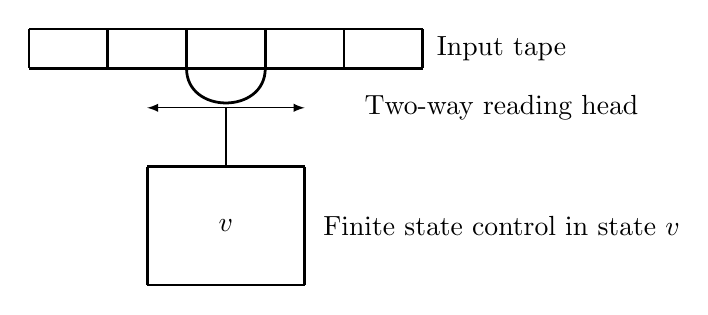
\begin{tikzpicture}
	\begin{pgfonlayer}{nodelayer}
		\node [style=none] (0) at (-1, -0.5) {};
		\node [style=none] (1) at (0, -0.5) {};
		\node [style=none] (2) at (-3, -0) {};
		\node [style=none] (3) at (-3, -0.5) {};
		\node [style=none] (4) at (2, -0) {};
		\node [style=none] (5) at (2, -0.5) {};
		\node [style=none] (6) at (-1, -0.5) {};
		\node [style=none] (7) at (0, -0.5) {};
		\node [style=none] (8) at (-1.5, -1.75) {};
		\node [style=none] (9) at (0.5, -1.75) {};
		\node [style=none] (10) at (-1.5, -3.25) {};
		\node [style=none] (11) at (0.5, -3.25) {};
		\node [style=none] (12) at (-0.5, -1) {};
		\node [style=none] (13) at (-0.5, -1.75) {};
		\node [style=none] (14) at (-0.5, -2.5) {$v$};
		\node [style=none] (15) at (3, -0.25) {Input tape};
		\node [style=none] (16) at (3, -1) {Two-way reading head};
		\node [style=none] (17) at (3, -2.5) {Finite state control in state $v$};
		\node [style=none] (18) at (-1.5, -1) {};
		\node [style=none] (19) at (0.5, -1) {};
		\node [style=none] (20) at (-2, -1) {};
		\node [style=none] (21) at (-2, -0) {};
		\node [style=none] (22) at (-2, -0.5) {};
		\node [style=none] (23) at (-1, -0) {};
		\node [style=none] (24) at (0, -0) {};
		\node [style=none] (25) at (1, -0) {};
		\node [style=none] (26) at (1, -0.5) {};
	\end{pgfonlayer}
	\begin{pgfonlayer}{edgelayer}
		\draw [style=simple] (3.center) to (0.center);
		\draw [style=simple] (0.center) to (1.center);
		\draw [style=simple] (1.center) to (5.center);
		\draw [style=simple, bend right=90, looseness=1.50] (6.center) to (7.center);
		\draw [style=simple] (6.center) to (7.center);
		\draw [style=simple] (8.center) to (9.center);
		\draw [style=simple] (9.center) to (11.center);
		\draw [style=simple] (11.center) to (10.center);
		\draw [style=simple] (10.center) to (8.center);
		\draw [style=simple] (12.center) to (13.center);
		\draw [style=transition] (12.center) to (18.center);
		\draw [style=transition] (12.center) to (19.center);
		\draw [style=simple] (2.center) to (4.center);
		\draw [style=simple] (21.center) to (22.center);
		\draw [style=simple] (23.center) to (0.center);
		\draw [style=simple] (24.center) to (1.center);
		\draw [style=simple] (25.center) to (26.center);
		\draw [style=simple] (4.center) to (5.center);
		\draw [style=simple] (2.center) to (3.center);
	\end{pgfonlayer}
\end{tikzpicture}
\end{center}

The representation of such an automaton by a state graph is not trivial. For
this reason, we first define this type of automaton as usual.

Afterwards, we will show how to represent this automaton by a state graph.

(The definition from the original book has been adapted to be closer to the
common namings.)

\begin{definition}
A {\bf (non-deterministic) two-way finite automaton} is defined by
\[ \fa{B} = (X, Q, \delta, S, F, \setof{L, R}) \]
where 
\begin{itemize}
  \item $X$ is the input alphabet with $\setof{L, R} \cap X = \emptyset$
  \item $Q$ is the state set with $\setof{L, R} \cap Q = \emptyset$
  \item $S \subset Q$ is the set of start states
  \item $F \subset Q$ is the set of final states of $\fa{B}$
  \item $\delta \subset (Q \times X) \to (Q \times \setof{L, R})$ is a
  relation describing the functioning of $\fa{B}$
\end{itemize}

If $\delta : (Q \times X) \to Q \times \setof{L, R}$ is a map, then
$\fa{B}$ is called a {\bf complete, deterministic two-way finite automaton}.
\end{definition}

\bigskip
\begin{definition}
A {\bf computation} of $\fa{B}$ on the input word $v \in X^*$ is a sequence of
single computation steps
\[ f_k = (q_0 v \to u_1 q_1 v_1 \to u_2 q_2 v_2 \to \ldots \to u_k q_k v_k) \]
with $u_i, v_i \in X^*,\ q_i \in Z$ for $i = 1, \ldots, k$ and $q_0 \in S$. 
\end{definition}

A single computation step $u_i q_i v_i \to u_{i+1} q_{i+1} v_{i+1}$ is defined
by the following alternatives:

\begin{itemize}
  \item If $v_i = a v'_i$, then $u_{i+1} = u_i a,\ v_{i+1} =
  v'_i$, if $(q_{i+1}, R) \in \delta(q_i, a)$,\\
  i.e.\ the reading head moves to the right and the automaton changes into state
  $q_{i+1}$, if it reads $a$ in state $q_i$.

	\item If $u_i = u'_i b,\ v_i = a v'_i$, then $u_{i+1} = u'_i$ and
	$v_{i+1} = b v_i$, if $(q_{i+1}, L) \in \delta(q_i, a)$,\\
	i.e.\ the reading head moves to the left and the automaton changes into state
	$q_{i+1}$, if it reads $a$ in state $q_i$.
\end{itemize}

\bigskip
\begin{definition}
A word $w \in X^*$ is {\bf accepted by} $\fa{B}$ if there exists a computation
$f_k$ with $v_k = \epsilon$ and $q_k \in F$.
\end{definition}

The language of $\fa{B}$ is
\[ L_{\fa{B}} = \setof{w \in X^* \mid w\text{ is accepted by }\fa{B}} \]

\bigskip
We want to consider again the monoid $\hgroup{X}$ (H-group, involutive monoid),
see chapter I.3, and construct an automaton 
\[ \fa{D} = (G, \hgroup{X}, S, F, \alpha) \]
with graph $G=(V, E)$ as follows:
\begin{itemize}
  \item $V = Q \times \setof{L_1, L_2, R_1, R_2}$
  
  \item Edge set $E$ and labelling $\alpha: E \to \hgroup{X}$ are defined as
  follows:
  
  $E$ contains an edge $e: (q, y) \edge{a} (q', y') \iff$ one of the following
  cases occurs:
  \begin{enumerate}
    \item $y = R_2,\ y' = R_2,\ (q', R) \in \delta(q, a)$
    \item $y = R_2,\ y' = L_1,\ (q', L) \in \delta(q, a)$
    \item $y = R_1,\ y' = R_2,\ q = q'$ and there exists $\bar{q} \in Q$ with
    $(q, R) \in \delta(\bar{q}, a)$
  \end{enumerate}

  $E$ contains an edge $e: (q, y) \edge{\inv{a}} (q', y') \iff$ one of the
  following cases occurs:
  \begin{enumerate}
    \item $y = L_2,\ y' = L_2,\ (q', L) \in \delta(q, a)$
    \item $y = L_2,\ y' = R_1,\ (q', R) \in \delta(q, a)$
    \item $y = L_1,\ y' = L_2,\ q = q'$ and there exists $\bar{q} \in Q$ with
    $(q, L) \in \delta(\bar{q}, a)$
  \end{enumerate}
\end{itemize}

\bigskip
To clarify this definition, we imagine the following model:

The input tape of the automaton is alternatingly divided into rectangular and
oval cells.

\begin{center}
\begin{tikzpicture}
	\begin{pgfonlayer}{nodelayer}
		\node [style=box] (0) at (0, -0) {$a$};
		\node [style=state] (1) at (-1, -0) {};
		\node [style=state] (2) at (1, -0) {};
		\node [style=state] (3) at (3, -0) {};
		\node [style=box] (4) at (4, -0) {$$};
		\node [style=state] (5) at (5, -0) {};
		\node [style=state] (6) at (-5, -0) {};
		\node [style=box] (7) at (-4, -0) {$$};
		\node [style=state] (8) at (-3, -0) {};
		\node [style=none] (9) at (-2, -0) {$\ldots$};
		\node [style=none] (10) at (2, -0) {$\ldots$};
		\node [style=none] (11) at (-4, 0.5) {$1$};
		\node [style=none] (12) at (0, 0.5) {$k$};
		\node [style=none] (13) at (4, 0.5) {$n$};
		\node [style=none] (14) at (-0.5, -1.5) {};
		\node [style=none] (15) at (0.5, -1.5) {};
		\node [style=none] (16) at (-0.5, -2.5) {};
		\node [style=none] (17) at (0.5, -2.5) {};
		\node [style=none] (18) at (0, -2) {$\fa{D}$};
		\node [style={triangle_down}] (19) at (1, -0.75) {};
		\node [style=none] (20) at (0, -1.5) {};
		\node [style=none] (21) at (1, -1) {};
	\end{pgfonlayer}
	\begin{pgfonlayer}{edgelayer}
		\draw [style=simple] (14.center) to (15.center);
		\draw [style=simple] (15.center) to (17.center);
		\draw [style=simple] (17.center) to (16.center);
		\draw [style=simple] (16.center) to (14.center);
		\draw [style=simple] (21.center) to (20.center);
		\draw [style=simple] (6) to (7);
		\draw [style=simple] (7) to (8);
		\draw [style=simple] (1) to (0);
		\draw [style=simple] (0) to (2);
		\draw [style=simple] (3) to (4);
		\draw [style=simple] (4) to (5);
	\end{pgfonlayer}
\end{tikzpicture}
\end{center}

The ovals represent ''idle-positions'' for the reading head, the rectangles
contain the single symbols of the input word.

The reading head moves from an ''idle-position'' to the neighbor
''idle-position'' to the left or to the right.

If it moves from left to right over the cell $k$ with symbol $a$, then the
automaton reads $a$, if it moves from right to left over that cell, it reads
$\inv{a}$. (This kind of reading when traversing a cell corresponds
to the physical model of a magnetic disc).

In some cases, our model has to perform two computation steps when the
automaton $\fa{B}$ performs only a single step.

The following cases may occur:

\begin{enumerate}
  \item The automaton is in idle position to the left of a cell $k$. It
  remembers that it should move to the right, i.e.\ it is in some state $(q,
  R_2)$. It traverses now the $k$th cell, reads the symbol $a$, reaches the
  subsequent idle position and finds that it should have gone to the left. This
  is desribed by the state $(q', L_1)$. Therefore it moves back to its previous
  idle position and changes into state $(q', L_2)$. Together it has read $a
  \inv{a}$.
  
  This kind of movement can be expressed using the following path:
  \[ (q, R_2) \edge{a} (q', L_1) \edge{\inv{a}} (q', L_2) \]
  
  \item In the same way, the following path is to be understood:
  \[ (q, L_2) \edge{\inv{a}} (q', R_1) \edge{a} (q', R_2) \]
\end{enumerate}

The definition of $\fa{D}$ is completed by setting
\[ S = S_{\fa{B}} \times \setof{R_2},\quad F = F_{\fa{B}} \times \setof{R_2} \]

We write again $|u| \in (\unioninv{X})^*$ for the reduced word for an element
$[u] \in \hgroup{X}$ and define:

\begin{definition}
\begin{eqnarray*}
\genbyone{L_{\fa{D}}} &:=& \{ |\alpha(\pi)| \mid  |\alpha(\pi)| \in
X^*,\ \pi \in \pathcat{G}(S, F) \\
&& \text{and for all paths prefixes }\omega \prefix \pi \text{ holds: }
|\alpha(\omega)| \prefix |\alpha(\pi)| \}
\end{eqnarray*}

Here, the symbol $\prefix$ denotes the path-prefix relation
\[ \prefix\ \subset \pathcat{G} \times \pathcat{G} \]
as well as the word-prefix relation
\[ \prefix\ \subset (\unioninv{X})^* \times (\unioninv{X})^* \]
\end{definition}

First, we want to give an example to clarify the construction given above.

The following two-way finite automaton accepts the language
\begin{eqnarray*}
L &=& \{ w \in \setof{a, b}^+ \cdot c \cdot \setof{a, b}^+ \mid w = w_1 \cdots
w_n,\ w_i \in X \\
&& \text{ with } w_i = c \Rightarrow w_{i-1} = w_{i+1},\ 1 < i < n \}
\end{eqnarray*} 

The transition function shall be defined as follows:
\begin{eqnarray*}
\delta(q_0, a) &=& \delta(q_1, a) = (q_1, R) \\
\delta(q_0, b) &=& \delta(q_1, b) = (q_1, R) \\
\delta(q_1, c) &=& (q_2, L) \\
\delta(q_2, a) &=& (q_a, R) \\
\delta(q_2, b) &=& (q_b, R) \\
\delta(q_a, c) &=& (q_{a'}, R) \\
\delta(q_b, c) &=& (q_{b'}, R) \\
\delta(q_{a'}, a) &=& (q_e, R) \\
\delta(q_{b'}, b) &=& (q_e, R) \\
\delta(q_{e}, a) &=& \delta(q_e, b) = q_e, R)
\end{eqnarray*}

The two-way finite automaton $\fa{A}$ is defined by
\[ \fa{A} = (\setof{q_0, q_1, q_2, q_a, q_b, q_{a'}, q_{b'}, q_e}, \setof{a,
b, c}, \setof{q_0}, \setof{q_e}, \delta) \]

From this we want to construct our automaton 
\[ \fa{D} = (G, \hgroup{\setof{a, b, c}}, \setof{(q_0, R_2)}, \setof{(q_e,
R_2)}, \alpha) \]

The graph $G = (V, E)$ has the following form (the markings at the edges are
the edge labels): 

\begin{center}
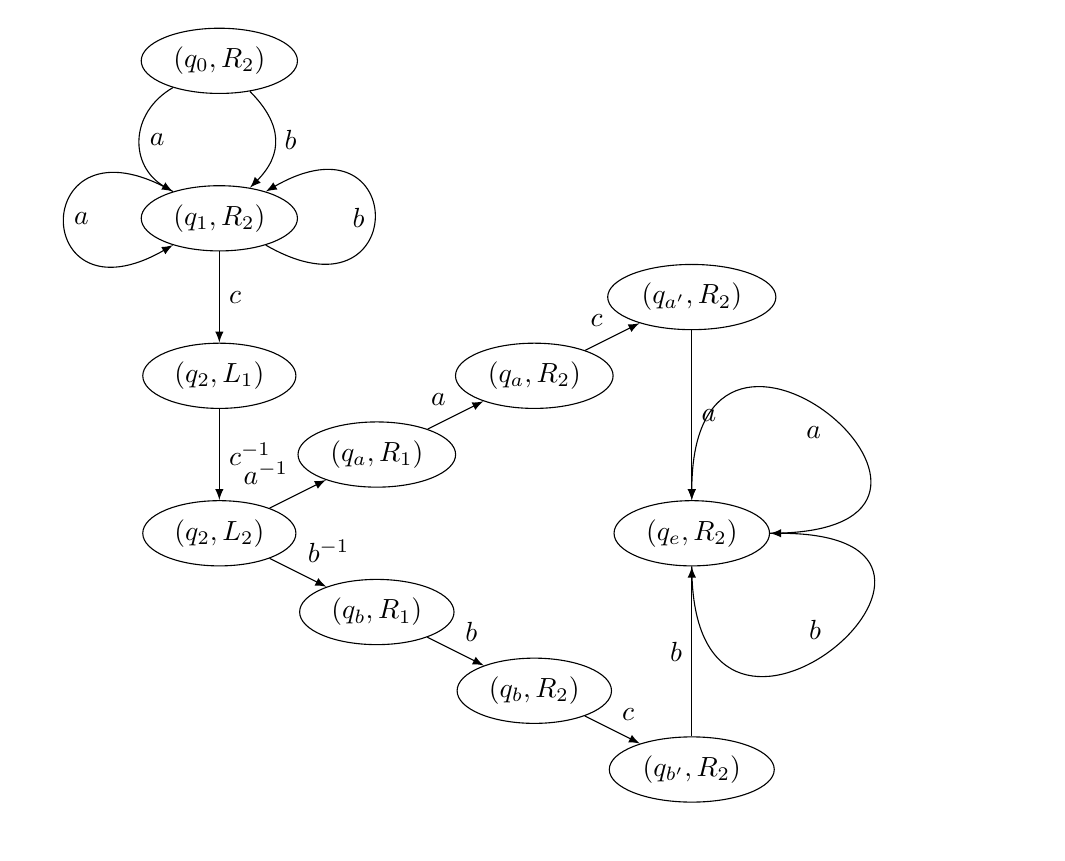
\begin{tikzpicture}
	\begin{pgfonlayer}{nodelayer}
		\node [style={oval_state}] (0) at (0, 6) {$(q_0, R_2)$};
		\node [style={oval_state}] (1) at (0, 4) {$(q_1, R_2)$};
		\node [style={oval_state}] (2) at (0, 2) {$(q_2, L_1)$};
		\node [style={oval_state}] (3) at (0, -0) {$(q_2, L_2)$};
		\node [style={oval_state}] (4) at (2, 1) {$(q_a, R_1)$};
		\node [style={oval_state}] (5) at (2, -1) {$(q_b, R_1)$};
		\node [style={oval_state}] (6) at (4, 2) {$(q_a, R_2)$};
		\node [style={oval_state}] (7) at (6, 3) {$(q_{a'}, R_2)$};
		\node [style={oval_state}] (8) at (6, -0) {$(q_e, R_2)$};
		\node [style={oval_state}] (9) at (4, -2) {$(q_b, R_2)$};
		\node [style={oval_state}] (10) at (6, -3) {$(q_{b'}, R_2)$};
	\end{pgfonlayer}
	\begin{pgfonlayer}{edgelayer}
		\draw [style=transition, bend right=60, looseness=1.25] (0) to node[auto]{$a$} (1);
		\draw [style=transition] (1) to node[auto]{$c$} (2);
		\draw [style=transition] (2) to node[auto]{$\inv{c}$} (3);
		\draw [style=transition] (3) to node[auto]{$\inv{a}$} (4);
		\draw [style=transition] (4) to node[auto]{$a$} (6);
		\draw [style=transition] (6) to node[auto]{$c$} (7);
		\draw [style=transition] (7) to node[auto]{$a$} (8);
		\draw [style=transition] (3) to node[auto]{$\inv{b}$} (5);
		\draw [style=transition] (5) to node[auto]{$b$} (9);
		\draw [style=transition] (9) to node[auto]{$c$} (10);
		\draw [style=transition] (10) to node[auto]{$b$} (8);
		\draw [style=transition, in=-150, out=150, loop] (1) to node[auto]{$a$} ();
		\draw [style=transition, in=30, out=-30, loop] (1) to node[auto]{$b$} ();
		\draw [style=transition, bend left=45, looseness=1.25] (0) to node[auto]{$b$} (1);
		\draw [style=transition, in=90, out=0, loop] (8) to node[auto]{$a$} ();
		\draw [style=transition, in=0, out=-90, loop] (8) to node[auto]{$b$} ();
	\end{pgfonlayer}
\end{tikzpicture}
\end{center}

We begin with proving the equivalence between both automata models. To do so, we
prove the following lemma.

\begin{lemma}
\[ L_{\fa{B}} \subset \genbyone{L_{\fa{D}}} \]
\end{lemma}

\begin{proof}
To each computation $f_k,\ k \in \mathbb{N}$, of the automaton
$\fa{B}$ we assign a path $\pi \in \pathcat{G}(S, V)$. We use induction over the
length of the computations.

{\em Induction base:}

To the empty computation $f_0$ we assign the empty path $1_{(q_0, R_2)}$ where
$q_0 \in S_{\fa{B}}$ is a start state of $\fa{B}$.

It holds: $\alpha(1_{(q_0, R_2)}) = \epsilon = u_0$.

{\em Induction step:}

For all computations $f_k$ of length $k$ we assume to have a path $\pi_k \in
\pathcat{G}(S, V)$ such that $Z(\pi_k) \in Q \times \setof{(R_2, L_2)}$ and
\[ |\alpha(\pi_k)| = \begin{cases}
u_k & \text{for }Z(\pi_k) \in Q \times \setof{R_2} \\
u_k \cdot First(v_k) & \text{for }Z(\pi_k) \in Q \times \setof{L_2}
\end{cases} \]

Here $First(w)$ denotes the first symbol of the word $w$.

Let $f_{k+1}$ be a computation of length $k+1$ which ends with the computation
step
\[ u_k q_k v_k \to u_{k+1} q_{k+1} v_{k+1} \]

\begin{itemize}
  \item[Case 1:] $Z(\pi_k) = (q_k, R_2),\ v_k = a \bar{v}_k,\ (q_{k+1}, R) \in
  \delta(q_k, a)$
  
  By construction, $G$ contains an edge $e: (q_k, R_2) \edge{a} (q_{k+1}, R_2)$.
  
  We set $\pi_{k+1} := \pi_k \cdot e$ and get
  \[ |\alpha(\pi_{k+1})| = |\alpha(\pi_k)| \cdot a = u_{k+1} \]
  
  \item[Case 2:] $Z(\pi_k) = (q_k, R_2),\ u_k = \bar{u}_k b,\ v_k = a
  \bar{v}_k,\ (q_{k+1}, L) \in \delta(q_k, a)$
  
  By construction, in $G$ there exists a path
  \[ (q_k, R_2) \edge{e_1 / a} (q_{k+1}, L_1) \edge{e_2 / \inv{a}} (q_{k+1},
  L_2),\ e_1, e_2 \in E \]
  
  We set $\pi_{k+1} := \pi_k \cdot e_1 \cdot e_2$, then it is
  \[ |\pi_{k+1}| = |\pi_k| = u_{k+1} \cdot b = u_{k+1} \cdot First(v_{k+1}) \]
  and $Z(\pi_{k+1}) \in Q \times \setof{L_2}$.
  
  \item[Case 3:] $Z(\pi_k) = (q_k, L_2),\ v_k = a \bar{v}_k,\ (q_{k+1}, R) \in
  \delta(q_k, a)$
  
  In $G$ there exists a path 
  \[ (q_k, L_2) \edge{e_1 / \inv{a}} (q_{k+1}, R_1) \edge{e_2 / a} (q_{k+1},
  R_2),\ e_1, e_2 \in E \]
  
  We set $\pi_{k+1} := \pi_k \cdot e_1 \cdot e_2$, then it is $Z(\pi_{k+1}) \in
  Q \times \setof{R_2}$ and
  \[ |\alpha(\pi_{k+1})| = |u_k a \inv{a} a| = u_k a = u_{k+1} \]
  
  \item[Case 4:] $Z(\pi_k) = (q_k, L_2),\ u_k = \bar{u}_k b,\ v_k = a
  \bar{v}_k,\ (q_{k+1}, L) \in \delta(q_k, a)$
  
  In $G$ there exists an edge $e: (q_k, L_2) \edge{\inv{a}} (q_{k+1}, L_2)$.
  
  We set $\pi_{k+1} := \pi_k \cdot e$, then $Z(\pi_{k+1}) = (q_{k+1}, L_2)$ and
  it is
  \[ |\alpha(\pi_{k+1})| = |\alpha(\pi_k)| \cdot \inv{a} = |u_k \cdot a \inv{a}|
  = |u_k| = u_{k+1} \cdot First(v_{k+1}) \]
\end{itemize}

These are all possible cases for $\pi_{k+1}$ and $\pi_{k+1}$ fulfills the
induction claim for $k+1$.

Let now $f_n$ be an accepting computation for a word $v$, so $v_n = \epsilon,\
u_n = v$ and $q_n \in F$.

The last move of $\fa{B}$ was a right-move. It holds $Z(\pi_n) = (q_n, R_2)$ and
therefore it holds $|\alpha(\pi_n)| = u_n = v$.

For each subpath $\omega$ of a path $\pi_n$ constructed in that way we get
\[ \forall \omega \prefix \pi_n \text{ it holds: }|\alpha(\omega)| \prefix
|\alpha(\pi_n)| \]

Because $f_n$ is an {\em accepting} computation, i.e.\ the reading head is
placed to the right of the right-most input symbol, each input symbol must have 
been traversed one time more often to the right than to the left.

This means, if a subpath $e \cdot e'$ with label $\alpha(e \cdot e') = a
\inv{a}$ exists in $\pi_n$, then it must be followed by an edge $e''$ with
$\alpha(e'') = a$.

The prefix condition of $\pi_n$ therefore cannot be violated by cancellation of
an edge labelled with $\inv{a}$.

It therefore holds: $|\alpha(\pi_n)| = u_n = v \in \genbyone{L_{\fa{D}}}$.
\end{proof}

\bigskip
\begin{lemma}
\[ \genbyone{L_{\fa{D}}} \subset L_{\fa{B}} \]
\end{lemma}

\begin{proof}
Let $G = (V, E)$ be the graph of $\fa{D}$, $v \in \genbyone{L_{\fa{D}}}$ and
$\pi \in \pathcat{G}(S, F)$ be a path with label $|\alpha(\pi)| = v$, and for
any path prefix $\omega \prefix \pi$ it should hold $|\alpha(\omega)| \prefix
|\alpha(\pi)|$.

We want to construct a computation $f$ which corresponds to the path $\pi$ in
the sense of the previous lemma.

We consider the sequence of subpaths
\[ 1_{(q_0, R_2)} \prefix \pi_1 \prefix \pi_2 \ldots \prefix \pi_n = \pi \]
with $\len{\pi_i} - \len{\pi_{i-1}} \leq 2$ and $Z(\pi_i) \in Q \times
\setof{R_2, L_2}$ for $i = 1, \ldots, n$ and for $\pi_i \prefix \omega \prefix
\pi_{i+1},\ \pi_i \neq \omega \neq \pi_{i+1}, \Rightarrow Z(\omega) \in Q \times
\setof{R_1, L_1}$.

We apply the automaton $\fa{B}$ on the input $v$ and show that there exists a
computation $f$ which corresponds to the path $\pi$.

\medskip
To the empty path $\pi_0 = 1_{(q_0, R_2)}$ corresponds the computation $q_0 v$.

Let $f_k$ be a computation ending with $u_k q_k v_k$.

Here, we also have to consider 4 cases:

\begin{itemize}
  \item[Case 1:] $Z(\pi_k) = (q_k, R_2),\ \pi_{k+1} = \pi_k \cdot e$ with $Z(e)
  = (q_{k+1}, R_2)$ and $\alpha(e) = a$.
  
  It then holds $v_k = a \bar{v}_k$ and by construction of $\fa{D}$ it holds
  $(q_{k+1, R}) \in \delta(q_k, a)$, therefore $u_{k+1} q_{k+1} v_{k+1}$ is
  a configuration following $u_k q_k v_k$.
   
  \item[Case 2:] $Z(\pi_k) = (q_k, R_2),\ \pi_{k+1} = \pi_k \cdot e_1 \cdot
  e_2$.
  
  We then have $Z(e_1) = (q_{k+1}, L_1),\ Z(e_2) = (q_{k+1}, L_2)$ and
  $\alpha(e_1) = a$ and $\alpha(e_2) = \inv{b}$.
  
  Because of $|\alpha(\pi)| \in X^*$ it follows $b = a$ and we have
  \[ (q_{k+1}, L) \in \delta(q_k, a)\text{ and }u_{k+1} = u \inv{a},\
  v_{k+1} = a v_k \]
  and $u_{k+1} q_{k+1} v_{k+1}$ is a configuration following $u_k q_k v_k$.
  
  \item[Case 3:] $Z(\pi_k) = (q_k, L_2),\ \pi_{k+1} = \pi_k \cdot e$.
  
  It then holds $Z(e) = (q_{k+1}, L_2)$ and $\alpha(e) \in \inv{X}$. Let
  $\alpha(e) = \inv{a}$. We then have $|\alpha(\pi_{k+1})| = |\alpha(\pi_k)
  \cdot \inv{a}|$. Because of $|\alpha(\pi| \in X^*,\ \pi \in \pathcat{G}(S, V)$
  and $|\alpha(\pi_k| = u_k \cdot First(v_k)$ it follows $First(v_k) = a$.
  
  If we have $u_k = \bar{u}_k b$, then for $u_{k+1} = \bar{u}_k$ and $v_{k+1} =
  b a v_k$ it holds: $u_{k+1} q_{k+1} v_{k+1}$ is a configuration following
  $u_k q_k v_k$.
  
  \item[Case 4:] $Z(\pi_k) = (q_k, L_2),\ \pi_{k+1} = \pi_k \cdot e_1 \cdot
  e_2$.
  
  It follows $Z(e_1) = (q_{k+1}, R_1)$ and $Z(e_2) = (q_{k+1}, R_2)$ and
  $\alpha(e_1) = \inv{a} \in \inv{X},\ \alpha(e_2) = b \in X$.
  
  Because of $\alpha(\pi) \in X^*,\ \pi \in \pathcat{G}(S, V)$ it follows
  $|\alpha(\pi_k)| = u_k a$ and because $u_k a \inv{a} b \prefix |\alpha(\pi)|$
  and $u_k a \prefix |\alpha(\pi_{k+1})|$ it follows $b = a$.
  
  Therefore $\alpha(\pi_{k+1}) = u_k a$. If we set $u_{k+1} = u_k a$ and
  $v_{k+1} = \inv{a} v_k\ (v_k = a \bar{v}_k)$, then by construction of
  $\fa{D}$, $u_{k+1} q_{k+1} v_{k+1}$ is a configuration following $u_k q_k v_k$
  and the path $\pi_{k+1}$ corresponds to the computation $f_k$.
\end{itemize}

Let $v \in \genbyone{L_{\fa{D}}}$ and $\pi_n \in \pathcat{G}(S, F)$ with label
$|\alpha(\pi_n)| = v$ and let for $\omega \prefix \pi_n$ hold $|\alpha(\omega)|
\prefix |\alpha(\pi_n)|$, then there exists a computation $f_n = (q_0 v \to
\ldots \to v q_n)$ with $q_0 \in S_{\fa{B}},q_n \in F_{\fa{B}}$ and therefore
$v \in L_{\fa{B}}$.
\end{proof}

Both lemmata are summarized in the following theorem:

\begin{theorem}
\[ L_{\fa{B}} = \genbyone{L_{\fa{D}}} \]
\end{theorem}

\bigskip
We will show now that for all finite two-way automata $\fa{B}$ it holds
\[ L_{\fa{B}} \in \reglang(X^*)\ (= \ratlang(X^*)) \]

Before doing that, we show a relationship between $\ratlang(X^*)$ and
$\ratlang(\hgroup{X})$.

For the automaton $\fa{D}$ constructed above we set
\[ L_{\fa{D}} := \setof{|\alpha(\pi)| \mid \pi \in \pathcat{G}(S, F)} \]
where $G = (V, E)$ is the graph of $\fa{D}$.

In this way, $\ratlang(\hgroup{X})$ is embedded in a natural way into
$(\unioninv{X})^*$, see chapter II.7.

We set
\[ |\ratlang(\hgroup{X})| := \setof{|L| \mid L \in \ratlang(\hgroup{X})} \]

Then the following theorem holds:

\begin{theorem}
\[ |L| \cap X^* \in \ratlang(X^*) \]
\end{theorem}

\begin{proof}
We only sketch the proof of this theorem, the reader may give the proof
formally.

Let $q_1, q_2$ be vertices of the graph $G = (V, E)$ of the automaton $\fa{D}$,
and let $\pi: q_1 \to q_2$ be a path with label $\alpha(\pi) \equiv 1
\pmod{\hgroup{X}}$.

In this case, a new edge $e: q_1 \edge{\epsilon} q_2$ will be added to the
graph. This will be done for all pairs $(q_1, q_2) \in V \times V$ which are
connected by such a path.

We get a new automaton $\fa{D}'$ with $|L_{\fa{D}}| = |L_{\fa{D}'}|$.

If one removes all edges $e$ from the graph of $\fa{D}'$ with label 
$\alpha(e) \in \inv{X}$, one gets a finite automaton $\fa{A}$ accepting the 
language $|L| \cap X^*$ (exercise).
\end{proof}

Remark: A similar result can be proved for the free group $F(X)$
(exercise).

\bigskip
\begin{theorem}[Rabin, Scott]
\[ \genbyone{L_{\fa{D}}} \in \reglang(X^*) \]
\end{theorem}

\begin{proof}
The proof gets clearer if we don't use the state graph but the automaton model
used in the construction of $\fa{D}$.

\missingfigure

On the input tape we have $w = x_1 \cdots x_n,\ x_i \in X$, the automaton shall
be in state $(q, y),\ y \in \setof{L_2, R_2})$ and the reading head shall be
located to the right of the $k$th cell.

We set $w_k := x_1 \cdots x_k$ and ask in which states the automaton will return
to its current position for $y = L_2$.

We denote the set of these states as the {\bf echo} of state $q$ in $w_k$.

We don't assume that the automaton has read the tape from the left, but think of
the head to be placed arbitrarily at this position in state $(q, L_2)$.

We define the echo formally:
\newcommand{\echo}[2]{\mathrm{Echo}_{#1}(#2)}

Define for $v \in X^*,\ a \in X$ the relation $\mathrm{Echo}_v \subset V \times
\powset{V}$ by
\begin{enumerate}
  \item $\echo{\epsilon}{(q, L_i)} = \emptyset$ for $i = 1, 2$.
  
  \item $\echo{v}{(q, R_i)} = (q, R_i)$ for $i = 1, 2$.
  
  \item $\echo{v \cdot a}{(q, L_1)} = a \cdot \echo{v}{(\inv{a}(q, L_1))}$
  
  \item $\echo{v \cdot a}{(q, L_2)} = (a \cdot \echo{v}{\inv{a}})^+ (q L_2)$
\end{enumerate}

\end{proof}































\chapter{Finite Automata with Storage}
\section{The finite automaton with pushdown store}

We investigate now a second example (after the 2-way automaton) that represents
a generalization of the finite automaton in our concept, the {\bf finite
automaton with pushdown store}.

For preparation we remember theorem 2 from chapter II.8

\begin{theorem}
For a finite automaton $\fa{A} = (G, \hgroup{X}, S, F, \alpha)$ it holds:
\[ X^* \cap |L_{\fa{A}}| \in REG(X^*) \]
\end{theorem}

Remark: From this theorem the following claims can be derived (exercise):
\begin{enumerate}
  \item With the same assumptions it holds $|L_{\fa{A}}| \in REG((X\cup
  X^{-1})^*)$
  \item Corresponding theorems hold for the free group $F(X)$ and the polycyclic
  monoid \pocymon{X} instead of \hgroup{X}.
\end{enumerate}
  
We want to introduce now the finite automaton with pushdown store. We define
\begin{definition}
$\pdstore{K} = (X, Y, \delta)$ is called {\bf simple pushdown store} with
input $X^*$ and stack-monoid $Y^*$ if
\begin{itemize}
  \item[(K1)] $\delta: X \times Y^* \to Y^*$ is a mapping with
  \begin{eqnarray*}
  \delta(X \times Y) & \subset & Y^2 \cup \{\epsilon\} \\
  \delta(X \times \{\epsilon\}) & \subset & Y
  \end{eqnarray*} 
  \item[(K2)] $\delta(x, u \cdot v) = u \cdot \delta(x, v)$ for $v \in Y^+,u \in
  Y^*$.
\end{itemize}
\end{definition} 

Obviously the simple pushdown store $\pdstore{K}$ is uniquely determined by
$\delta' = \delta |_{X \times (Y \cup \{\epsilon\})}$. Each such mapping can be
continued using (K2) onto $X \times Y^*$ such that one gets a simple
pushdown store.

We extend $\delta$ onto $X^* \times Y^*$ by defining
\begin{eqnarray*}
\delta(\epsilon, u) & = & u \\
\delta(x v, u) & = & \delta(v,  \delta(x,u))
\end{eqnarray*}

The following lemma holds:
\begin{lemma}
For $u \in \hgroup{X}$ there exists a pushdown store
\[ \pdstore{K} =(\unioninv{X}, \unioninv{X}, \delta) \]
with $|u| = \delta(u, \epsilon)$.
\end{lemma}

\begin{proof}
Define
\begin{eqnarray*}
\delta(x, \epsilon) & = & x,\ x\in \unioninv{X}\\
\delta(x, y) & = & x y,\ x\neq y^{-1}\\
\delta(x^{-1}, x) & = & \epsilon,\ x\in X
\end{eqnarray*}

Let $u\in (\unioninv{X})^*$ and $u = x_1^{\epsilon_1} \cdots x_n^{\epsilon_n}$
with $x_i\in X,\ \epsilon_i\in \{1, -1\}$.

For the sequence $y_1 = \delta(x_1^{\epsilon_1}, \epsilon),\ y_2 =
\delta(x_2^{\epsilon_2}, y_1), \ldots,\ y_n = \delta(x_n^{\epsilon_n}, y_{n-1})$
it holds: $y_n = |u|$ (exercise).
\end{proof}

Remark:
\begin{enumerate}
  \item The lemma holds also for the free group $F(X)$.
  \item The lemma does not hold for the polycyclic monoid $\pocymon{X}$
  (exercise).
\end{enumerate}

The reader should extend the definition of the pushdown store to a
pushdown store with 0 such that the lemma holds also for the polycyclic monoid
$\pocymon{X}$.

We can now define the finite automaton with pushdown store.

\begin{definition}
$\kappa = (\fa{A}, \pdstore{K})$ is called {\bf finite automaton with
pushdown store} or short {\bf PDA}, if $\fa{A} = (G, X, S, F, \alpha)$ is a
finite automaton with graph $G = (V, E)$ and $\pdstore{K} = (E, Y,\delta)$ is a
simple pushdown store.
\end{definition}

Two sets are assigned to the PDA $\kappa$, the {\bf pushdown class}
$KKL(\kappa)$ which is the set of possible words on the pushdown store when
$\fa{A}$ accepts a word, and the {\bf accepted language} $L_\kappa$ which is the
set of input words accepted with empty pushdown store.

Formally:
\begin{eqnarray*}
KKL(\kappa) &:=& \{ \delta(\pi, \epsilon) \mid \pi \in \pathcategory{G}(S, F) \} \\
L_\kappa &:=& \{ \alpha(\pi) \mid \pi \in \pathcategory{G}(S, F),\ \delta(\pi,
\epsilon) = \epsilon \}
\end{eqnarray*}

\begin{definition}
\[ ALG(X_\infty^*) := \{ L \subset X_\infty^* \mid \text{there exists a PDA
$\kappa$ with $L = L_\kappa$} \]
is called the class of {\bf algebraic languages}.
\end{definition}

The pushdown-class $KKL(\kappa)$ is an example for our concept of generalizing
the finite automata by changing the monoid. If we assign to each $x\in X$ a
mapping $\delta_x: Y^* \to Y^*$, then we can represent $\kappa$ by
\[ \fa{B} = (G, M, S, F, \beta) \]
where $M = \{ \delta_x \mid x\in X \}^*$ and $\beta(x) = \delta_x$.

It holds:
\[ L_{\fa{B}}(\epsilon) := \{ \beta(\pi)(\epsilon) \mid \pi \in
\pathcategory{G}(S, F) \} = KKL(\kappa) \]

As our main result we get
\begin{theorem}
\[ KKL(\kappa) \in REG(Y^*) \]
\end{theorem}

Before starting with the formal proof we want to explain the construction of the
automaton for $KKL(\kappa)$ using an example.

Let $\pi = (e_1 e_2 e_3 e_4 e_5 e_6 e_7 e_8)$ a path from \pathcategory{G} and the
pushdown store be empty initially.

$\delta$ shall be defined as follows:
\[\begin{array}{r@{\,=\,}l@{\qquad}r@{\,=\,}l@{\qquad}r@{\,=\,}l}
\delta(s_1,\epsilon)&y_1 & \delta(s_2,y_1)&y_1y_2 & \delta(s_3,y_2)&y_2y_3 \\
\delta(s_4,y_3)&\epsilon & \delta(s_5,y_2)&y_2y_4 & \delta(s_6,y_4)&\epsilon \\
\delta(s_7,y_2)&\epsilon & \delta(s_8,y_1)&y_1y_5
\end{array}\]

We assign to the computation of the pushdown store a word $w' \in (Y\cup
Y^{-1})^*$. The reduced word is the current content of the pushdown store,
hereby we have to guess in $w'$ the last symbol of the reduced word
(corresponds to the symbol on top of the stack).

Let a path $\pi \in \pathcategory{G},\ G=(V,E),$ be of the form
\[ \edge{e_1} \edge{e_2} \edge{e_3} \edge{e_4} \edge{e_5} \edge{e_6} \edge{e_7}
\edge{e_8} \]

In the automaton to be constructed we will have the following marking
\[ \edge{y_1} \edge{y_1^{-1} y_1 y_2} \edge{y_2^{-1} y_2 y_3} \edge{y_3^{-1}
y_2^{-1} y_2} \edge{y_2^{-1} y_2 y_4} \edge{y_4^{-1} y_2^{-1} y_2}
\edge{y_2^{-1} y_1^{-1} y_1} \edge{y_1^{-1} y_1 y_5}
\]

The first inverse on each edge label is used to ''guess'' the top symbol on
the stack.

The corresponding stack contents are:
\[ y_1 \qquad y_1 y_2 \qquad y_1 y_2 y_3 \qquad y_1 y_2 \qquad y_1 y_2 y_4
\qquad y_1 y_2 \qquad y_1 \qquad y_1 y_5 \qquad \]

By multiplying the edge labels and applying the cancellation rules one gets the
stack contents.

We want to execute this idea formally:

For the proof we construct an automaton $\fa{C}$ over the H-group $\hgroup{Y_0}$
where $Y_0 := Y \cup \setof{y_0},\ y_0 \notin Y$ and the property
\[ Y_0^* \cap |L_{\fa{C}}| = y_0 \cdot KKL(\kappa) \]

From theorem 1 then follows that $y_0 \cdot KKL(\kappa)$ is regular and from
this follows immediately $KKL(\kappa) \in REG(Y^*)$.

\transrem{The proof in the book was completely unreadable to me. Therefore I
used new names, added comments and figures.}

\begin{proof}
Let $\kappa = (\fa{A}, \pdstore{K})$ be a PDA with finite automaton
\[ \fa{A} = (G, X, S, F, \alpha) \]
with graph $G = (V, E)$ and pushdown store $\pdstore{K}$.

We define a finite automaton $\fa{C}$ with the H-group over $Y_0$ as its storage
monoid:
\[ \fa{C} = (G', \hgroup{Y_0}, \setof{s_0}, F, \gamma) \]

The graph $G'=(V',E')$ of $\fa{C}$ is defined as follows:

The vertices are the same as in $G$ plus a new vertex $s_0$ which becomes the
start state of $\fa{C}$:
\[ V' = V \cup \setof{s_0},\ s_0 \notin V \]

The edge set $E'$ contains three different types of edges:
\[ E' = \underbrace{\setof{s_0} \times S}_{\text{start edges}} \quad\cup\quad
\underbrace{E \times Y_0}_{\text{push-edges}} \quad\cup\quad \underbrace{E
\times Y \times Y_0}_{\text{pop-edges}}
\]

{\bf Start edges:} These edges provide the initial
stack content (bottom-of-stack symbol $y_0$).

For each start state $s \in S$ of the PDA $\kappa$ we define an edge
\[ e': s_0 \edge{y_0} s\]
formally:
\[ Q(e') = s_0,\quad Z(e') = s,\quad \gamma(e') = y_0 \]

\bigskip
{\bf Edges for simulating push-operations:} These edges simulate a
push-operation on the stack.
The top-most stack symbol $y$ is ''guessed'' and if the guess was correct, $y$ is
restored and $z$ is pushed on the stack. A wrong guess results in a combination of symbols on 
the stack that cannot be reduced to the empty word (no accepting computation
possible) anymore.
 
For each pair $(e, y) \in E \times Y$ there is an edge
\[ e': Q(e) \edge{y^{-1} y z} Z(e)\]
but only if the pushdown store does not compute the monoid unit for the edge,
formally $|\delta(e, y)| \neq \epsilon$. That means, the pushdown store indeed
puts a symbol on the stack when executing the transition $e$.

\bigskip
{\bf Edges for handling empty stack:} These edges simulate computations with
empty stack. The bottom-of-stack symbol is guessed and if the guess was correct, the
corresponding stack operation is simulated.

For each edge $e \in E$ we define an edge
\[ e': Q(e) \edge{y_0^{-1} y_0 \delta(e, \epsilon)} Z(e) \] 

\bigskip
{\bf Edges for simulating pop-operations:} These edges simulate popping of
symbols from the stack.
The top-most stack symbol $y$ is guessed and if the guess was correct, each
possible symbol $z$ that could be on the stack after popping $y$ is provided as
a possible continuation. If some symbol can never be on the stack after
popping $y$ the computation can never be successful. 

For each triple $(e, y, z) \in E \times Y
\times Y_0$ we define an edge
\[ e': Q(e) \edge{y^{-1} z^{-1} z} Z(e) \]
but only if the pushdown store pops the symbol $y$ when executing the transition
$e$, formally $\delta(e, y) = \epsilon$.

\bigskip
This completes the definition of the finite automaton $\fa{C}$.

We prove first that each accepting computation of the pushdown store may be
simulated with the finite automaton $\fa{C}$:
\[ y_0 \cdot KKL(\kappa) \subset |L_{\fa{C}}| \]

To prove this, we construct for each accepting path $\pi \in
\pathcategory{G}(S,F)$ an accepting path $\pi' \in
\pathcategory{G'}(\setof{s_0}, F)$ with $|y_0 \cdot \delta(\pi, \epsilon)| = |\gamma(\pi')|$ 
which means that the computation of the pushdown store is equivalent modulo the
H-group to the label of the computation path in $\fa{C}$.

Given an accepting computation $\pi$ in the PDA, we consider all prefixes
$\psi$ of $\pi$ by increasing length. The corresponding prefix of path $\pi'$ in
graph $G'$ will be denoted by $\psi'$.

{\em Induction base:} For prefix $\psi$ of length 0, that is $\psi =
(Q(\pi), Q(\pi))$, we set $\psi' := s_0 \edge{y_0} Q(\pi)$, that
is an edge from the start state $s_0$ to the start vertex of $\pi$. 

We get $\delta(\psi, \epsilon) = \delta(\epsilon, \epsilon) = \epsilon$ and
$\gamma(\psi') = y_0$ which proves the claim for paths of zero length.

{\em Induction step:} We assume that the two prefixes $\psi$ and $\psi'$ have
the same target vertex, $Z(\psi) = Z(\psi')$, and that the computations for
these prefixes fulfill the induction assumption, namely $|\gamma(\psi')| =
|y_0 \cdot \delta(\psi, \epsilon)|$.

Consider the path $\pi = \psi \circ e$ where $e$ is an edge of $G$ and let
$|y_0 \cdot \delta(\psi, \epsilon)| = u \cdot y$ for some symbol $y \in Y_0$.

We have two cases.

{\em Case 1}: $y \in Y$ and $\delta(e, y) = y z$:

By construction of $G'$ there exists an edge $e': Q(e) \edge{y^{-1} y z} Z(e)
\in E \times Y$.

Therefore we have $|y_0 \cdot \delta(\psi \circ e, \epsilon)| = |y_0 \cdot u
\cdot$




\end{proof}





























\section{Closure properties of $ALG(X^*)$}

In the last section we defined $ALG(X^*)$ as the class of languages over an
alphabet $X$ accepted by a pushdown automaton.

The name ''algebraic languages'' remembers the fact that these languages can be
defined as the solution of equation systems with non-commutative variables using
formal power series. See for example \cite{SaSo} or \cite{Berstel77}.

We will prove for $ALG(X^*)$ similar closure properties as for $\reglang(X^*)$.

In this section we assume without loss of generality that the pushdown automata
have the following properties:

$\card{S} = \card{F} = 1$ and no edge ends in a start state and no edge leaves a
final state. Additionally, all edges labels have length 0 or 1, $\alpha(e) \leq
1,\ e \in E$.

In a very easy way one gets

\begin{theorem}[Closure under monoid homomorphism]
\label{alg-lang-closure-hom}
Let $\phi : X^* \to Y^*$ be a monoid homomorphism.
\[ L \in ALG(X^*) \Rightarrow \phi(L) \in ALG(Y^*) \]
\end{theorem} 

\begin{proof}
$L \in ALG(X^*) \Rightarrow$ there exists a PDA $\kappa = (\fa{A}, \pdstore{K})$
with $L_{\kappa} = L$. Replace $\alpha$ by $\alpha' := \alpha \circ \phi$ in
the definition of $\fa{A}$. 

For
\[ \fa{A'} = (G, Y, S, F, \alpha') \]
the PDA $\kappa' = (\fa{A'}, \pdstore{K})$ accepts $\phi(L_{\kappa}) = \phi(L)$.
\end{proof}

\transrem{I changed names in the following proof for better readability.}

\bigskip
\begin{theorem}
$ALG(X^*)$ is closed under union, concatenation and Kleene-star.
\end{theorem}

{\em Closure under union:}
\[ L_1, L_2 \in ALG(X^*) \Rightarrow L_1 \cup L_2 \in ALG(X^*) \]
\begin{proof}
Let
\[ \kappa_1 = (\fa{A}_1,\pdstore{K}_1),\quad \fa{A}_1 = (G_1, X,
\setof{s_1}, \setof{f_1}, \alpha_1),\quad G_1 = (V_1, E_1),\quad \pdstore{K}_1 =
(X, Y_1, \delta_1)
\]
and
\[ \kappa_2 = (\fa{A}_2,\pdstore{K}_2),\quad \fa{A}_2 = (G_2, X,
\setof{s_2}, \setof{f_2}, \alpha_2),\quad G_2 = (V_2, E_2),\quad \pdstore{K}_2 =
(X, Y_2, \delta_2)
\]
be pushdown automata accepting $L_1$ resp.\ $L_2$.

We may assume that $Y_1 \cap Y_2 = \emptyset,\ E_1 \cap E_2 =
\emptyset,\ V_1 \cap V_2 = \setof{s_1, f_2}$ where $s_1 = s_2$ and $f_1 = f_2$.

Define the PDA $\kappa_1 \cup \kappa_2$ by
\[ \fa{A}_1 \cup \fa{A}_2 := (G_1 \cup G_2, X, \setof{s_1}, \setof{f_2},
\alpha_1 \cup \alpha_2) \]
and pushdown store
\[ \pdstore{K}_1 \cup \pdstore{K}_2 := (E_1 \cup E_2, Y_1 \cup Y_2 \cup
\setof{\infty}, \delta_1 \cup \delta_2) \]
where
\[ (\delta_1 \cup \delta_2)(e, y) = \begin{cases}
\delta_1(e, y) & e \in E_1,\ y \in Y_1 \cup \setof{\epsilon} \\ 
\delta_2(e, y) & e \in E_2,\ y \in Y_2 \cup \setof{\epsilon} \\
\infty\infty & \text{else} 
\end{cases}
\]

The symbol $\infty$ is only introduced to make $\delta_1 \cup \delta_2$
complete. If $\infty$ is on-top of the pushdown store, then this cannot become
empty anymore. In that way it will become impossible to ''mix'' words from both
languages.

It holds: $L_{\kappa_1 \cup \kappa_2} = L_{\kappa_1} \cup L_{\kappa_2}$
(exercise).

The following figure shows our construction:

FIGURE

\end{proof}

{\em Closure under complex product:}
\[ L_1, L_2 \in ALG(X^*) \Rightarrow L_1 \cdot L_2 \in ALG(X^*) \]
\begin{proof}
We construct the PDA $\kappa = (\fa{A}, \pdstore{K})$ with 
\[\fa{A} = (G, X, \setof{s_1}, \setof{f_2}, \alpha)\]
where
\begin{eqnarray*}
G &=& (V, E) \\
V &=& V_1 \cup V_2 \cup \setof{p},\ p \notin V_1 \cup V_2 \\
E &=& E_1 \cup E_2 \cup \setof{b_1, b_2},b_1, b_2 \notin E_1 \cup E_2
\end{eqnarray*}

For the new ''bridge'' edges $b_1, b_2$ it holds $b_1: f_1 \edge{\epsilon} p$
and $b_2: p \edge{\epsilon} s_2$.

The labeling of the graph $G$ is defined by 
\[ \alpha(e) = \begin{cases} 
\alpha_1(e) 	& e \in E_1 \\
\alpha_2(e) 	& e \in E_2 \\
\epsilon 			& e \in \setof{b_1, b_2} 
\end{cases}\]

FIGURE

The pushdown store $\pdstore{K} = (E, Y, \delta)$ is defined by
\[ Y = Y_1 \cup Y_2 \cup \setof{\Join, \infty} \text{ with }\setof{\Join, \infty} \cap
(Y_1 \cup Y_2) = \emptyset \]

\[ \delta(e, y) = \begin{cases}
\delta_1(e, y) 					& e \in E_1,\ y \in Y_1 \cup \setof{\epsilon} \\
\delta_2(e, y) 					& e \in E_2,\ y \in Y_2 \cup \setof{\epsilon} \\
y \cdot \Join 					& e = b_1,\ y \in Y \cup \setof{\epsilon} \\
\epsilon 								& e = b_2,\ y = \Join \\
\infty\infty 						& \text{else}
\end{cases}\]

We prove now that the pushdown automaton $\kappa$ defined in that way accepts
the complex product $L_1 \cdot L_2$.

''$L_1 \cdot L_2 \subset L_{\kappa}$'':

Let $w \in L_1 \cdot L_2$. Then there exists a factorization $w = w_1 \cdot
w_2,\ w_1 \in L_1, w_2 \in L_2$.

For $w_1$ there exists an accepting path $\pi_1 \in \pathcat{G_1}(s_1,
f_1)$ with label $\alpha_1(\pi_1) = w_1$ and pushdown store computation
$\delta_1(w_1, \epsilon) = \epsilon$.

For $w_2$ there exists an accepting path $\pi_2 \in \pathcat{G_2}(s_2,
f_2)$ with label $\alpha_2(\pi_2) = w_2$ and pushdown store computation
$\delta_2(w_2, \epsilon) = \epsilon$.

Consider the path $\pi = \pi_1 \circ b_1 \circ b_2 \circ \pi_2 \in
\pathcat{G}(s_1, f_2)$.

It holds
\begin{eqnarray*}
\delta(\pi) &=& \delta(\pi_1 \circ b_1 \circ b_2 \circ \pi_2) \\
&=& \delta(b_1 \circ b_2 \circ \pi_2, \delta(\pi, \epsilon)) \\
&=& \delta(b_1 \circ b_2 \circ \pi_2, \epsilon) \\
&=& \delta(b_2 \circ \pi_2, \delta(b_1, \epsilon)) \\
&=& \delta(b_2 \circ \pi_2, \epsilon \cdot \Join) \\
&=& \delta(\pi_2, \delta(b_2, \Join)) \\
&=& \delta(\pi_2, \epsilon) \\
&=& \delta_2(\pi_2, \epsilon) \\
&=& \epsilon
\end{eqnarray*}

This means, the pushdown store computation for $\pi$ is accepting.

The label of path $\pi$ is
\begin{eqnarray*}
\alpha(\pi) &=& \alpha(\pi_1 \circ b_1 \circ b_2 \circ \pi_2) \\
&=& \alpha(\pi_1) \circ \alpha(b_1) \circ \alpha(b_1 \circ \alpha(\pi_2) \\
&=& w_1 \cdot \epsilon \cdot \epsilon \cdot w_2 \\
&=& w_1 \cdot w_2 \\
&=& w
\end{eqnarray*}

This proves $w \in L_{\kappa}$ and therefore $L_1 \cdot L_2 \subset L_{\kappa}$.

''$L_1 \cdot L_2 \supset L_{\kappa}$'':

Let $w \in L_{\kappa}$ be a word accepted by the PDA $\kappa$. Then there exists
a path $\pi \in \pathcat{G}(s_1, f_2)$ with label $\alpha(\pi) = w$ and a
pushdown store computation $\delta(\pi, \epsilon) = \epsilon$.

The path $\pi$ has a unique factorization $\pi = \pi_1 \circ b_1 \circ b_2
\circ \pi_2$ with $\pi_1 \in \pathcat{G_1}(s_1, f_1)$ and $\pi_2 \in
\pathcat{s_2, f_2}$. 

Consider $\delta(\pi_1, \epsilon)$, the computation of the pushdown store on the
path prefix $\pi_1$:

Assume $\delta(\pi_1, \epsilon) \neq \epsilon$. Then $\delta(\pi_1 \circ b_1
\circ b_2 \circ \pi_2, \epsilon) = \delta_1(\pi, \epsilon)$

TODO clarify

For the path labels we have $\alpha_1(\pi_1) = w_1 \in L_1, \alpha_2(\pi_2) =
w_2 \in L_2$ and
\begin{eqnarray*}
\alpha(\pi) &=& \alpha(\pi_1 \cdot b_1 \cdot b_2 \cdot \alpha_2) \\
&=& \alpha(\pi_1) \cdot \epsilon \cdot \epsilon \cdot \alpha(\pi_2) \\
&=& w_1 \cdot w_2 \\
&=& w
\end{eqnarray*}

So $w \in L_1 \cdot L_2$ and $L_1 \cdot L_2 \supset L_{\kappa}$.
\end{proof}

{\em Closure under Kleene-star:}
\[ L \in ALG(X^*) \Rightarrow L^* \in ALG(X^*) \]
\begin{proof}
Let $\kappa = (\fa{A}, \pdstore{K})$ be a PDA accepting $L$. We construct a PDA
$\kappa'$ accepting $L^*$ as follows:
\[ \fa{A}' = (G, X, \setof{s}, \setof{f}, \alpha')\]
with
\begin{eqnarray*}
G' &=& (V', E') \\
V' &=& V \cup \setof{p, q},\ \setof{p, q} \cap E = \emptyset \\
E' &=& E \cup \setof{e_0, e_0', e_1, e_1'},\ \setof{e_0, e_0', e_1, e_1'} \cap E
= \emptyset \\
\end{eqnarray*}

The new edges have the following source, target states and labeling:
\begin{eqnarray*}
& e_0: s \edge{\epsilon} p \\
& e_0': s \edge{\epsilon} f \\
& e_1: f \edge{\epsilon} q \\
& e_1': q \edge{\epsilon} s \\
\end{eqnarray*}

FIGURE

The pushdown store $\pdstore{K}' = (E', Y', \delta')$ is defined by $Y' = Y
\cup \setof{y', y'', \infty}$ where $\setof{y', y'', \infty} \cap Y =
\emptyset$ and $\delta'$ defined by
\[ \delta'(e, y) = \begin{cases}
\delta(e, y)		& e \in E,\ y \in  Y \cup \setof{\epsilon} \\
y'							& e = e_0,\ y = \epsilon \\
\epsilon				& e = e_0',\ y = y' \\
y''							& e = e_1,\ y = \epsilon \\
\epsilon				& e = e_1',\ y = y'' \\
\infty\infty		& \text{else}
\end{cases}\]

For the so defined PDA $\kappa'$ we show $L^* = L_{\kappa'}$.

''$L^* \subset L_{\kappa}$'':

Let $w \in L^*$, then we have two cases:

\begin{enumerate}
  \item $w = \epsilon$: Then there exists the path $\pi = e_0 \circ e_0' \in
  \pathcat{G'}(s, f)$ with label $\alpha(\pi) = \epsilon$ and
  pushdown computation $\delta'(\pi) = \epsilon$.
  \item $w \neq \epsilon$: Then there exists a factorization $w = w_1 \cdots
  w_k,\ w_i \in L$ and paths $\pi \in \pathcat{G}(s, f)$ with labels
  $\alpha(\pi_i) = w_i$ and pushdown computations $\delta(\pi, \epsilon) =
  \epsilon,\ i = 1, \ldots, k$.
  
  Consider the path $\pi = \pi_1 \circ e_1 \circ e_1' \circ \pi_2 \circ e_1
  \circ e_1' \ldots \circ e_1 \circ e_1' \circ \pi_k \in \pathcat{G'}(s,
  f)$.
  
  It holds
  \begin{eqnarray*}
  \alpha(\pi) &=& \alpha(\pi_1) \cdot \alpha(e_1 \circ e_1') \cdot \alpha(\pi_2)
  \cdots \alpha(e_1 \circ e_1') \cdot \alpha(\pi_k) \\
  &=& \alpha(\pi_1) \cdot \epsilon \cdot \alpha(\pi_2) \cdots \epsilon \cdot
  \alpha(\pi_k)  \\
  &=& w_1 \cdots w_k = w
  \end{eqnarray*}
  
  For the pushdown computation holds:
  \begin{eqnarray*}
  \delta'(\pi, \epsilon) &=& \delta'(e_1 \circ e_1' \circ \pi_2 \ldots \pi_k,
  \delta(\pi_1, \epsilon)) \\
  &=& \delta'(e_1' \circ \pi_2 \ldots \pi_k, y'') = \delta'(\pi_2 \ldots \pi_k,
  \epsilon) \\
  &\ldots& \\
  &=& \delta'(\pi_k, \epsilon) = \delta(\pi_k, \epsilon) = \epsilon
  \end{eqnarray*}
 
  From this follows $w \in L_{\kappa'}$.
\end{enumerate} 
 
''$L^* \supset L_{\kappa}$'':

Let $w \in L_{\kappa'}$ be a word accepted by the PDA $\kappa'$. Then there
exists a path $\pi \in \pathcat{G'}(s, f)$ with label $\alpha'(\pi) = w$
and pushdown computation $\delta'(\pi, \epsilon) = \epsilon$.

\begin{enumerate}
  \item $\pi = e_0 \circ e_0',\ \alpha'(\pi) = \epsilon,\ \delta'(\pi, \epsilon)
  = \epsilon \Rightarrow \epsilon \in L^*$.
  
  \item Given a factorization $\pi = \pi_1 \circ e_1 \circ e_1' \circ \pi_2 \circ e_1
  \circ e_1' \ldots \circ e_1 \circ e_1' \circ \pi_k$ with $\pi_i \in
  \pathcat{G}(s, f)$ and edges $e_1, e_1'$ as constructed.
  
  Claim: $\delta'(\pi, \epsilon) = \epsilon \Rightarrow \delta(\pi_1, \epsilon)
  = \epsilon$
  
  Assumption: $\delta(\pi, \epsilon) \neq \epsilon$. Then by definition of
  $\delta'$ it holds $\delta'(e_1, \delta(\pi_1, \epsilon)) = \infty\infty$ and
  because $\delta'(e, \infty) = \infty\infty$ the pushdown store will never
  become empty, therefore $\delta'(\pi, \epsilon) \neq \epsilon$.
  
  This holds inductively for the paths $\pi_i,\ i = 1, \ldots k$. We get
  \begin{eqnarray*}
  \delta'(\pi, \epsilon) &=& \delta'(\pi_1 \circ e_1 \circ e_1' \circ \pi_2
  \ldots \pi_k, \epsilon) \Rightarrow \\
  \delta'(\pi_1, \epsilon) &=& \epsilon \\
  \delta'(\pi_1 \circ e_1 \circ e_1', \epsilon) &=& \delta'(e_1 \circ e_1',
  \delta(\pi_1, \epsilon)) = \delta'(e_1', y'') = \epsilon
  \end{eqnarray*}
  and for all $i = 1, \ldots, k:\ \delta'(\pi_i, \epsilon) = \epsilon$. 
  
  It holds $\alpha(\pi_i) = w_i \in L,\ i = 1, \ldots, k$.
  
  $\alpha'(\pi_1 \circ e_1 \circ e_1' \circ \pi_2 \ldots \pi_k) = \alpha(\pi_1)
  \cdot \epsilon \ldots \epsilon \cdot \alpha(\pi_k) = w_1 \cdots w_k = w \in
  L^*$.
\end{enumerate}

This completes the proof of our theorem.
\end{proof}

\bigskip
\begin{theorem}[Closure under intersection with regular language]
\label{alg-lang-closure-reg-intersect}
\[ L \in ALG(X^*),\ R \in \reglang(X^*)\Rightarrow L \cap R \in ALG(X^*) \]
\end{theorem}

\begin{proof}
Let $\kappa = (\fa{A}, \pdstore{K})$ be a PDA with $L_{\kappa} = L$ and $\fa{B}$
a complete, deterministic finite automaton accepting $R$. At each vertex, a loop
labeled with $\epsilon$ should be attached.

We construct a finite automaton $\fa{C} = \fa{A} \times \fa{B}$ as we did for
the intersection of regular languages in chapter II.1. The graph of $\fa{C}$ is
$G = (V, E)$ where the vertex set $V$ is the cartesian product $V_{\fa{A}}
\times V_{\fa{B}}$ and the edges are defined by
\[ E = \setof{(e, e') \in E_{\fa{A}} \times E_{\fa{B}} \mid \alpha(e) =
\beta(e') } \]

Because $\fa{B}$ is complete and deterministic, it holds $L_{\fa{C}} =
L_{\fa{A}} \cap L_{\fa{B}}$.

Now let $\kappa' = (\fa{C}, \pdstore{K}')$ be a PDA with $\pdstore{K}' = (E,
Y, \delta')$ and $\delta'((e, e'), y) = \delta(e, y)$.
For a word $w \in L_{\kappa'}$ there exists a path $\pi \in
\pathcat{G}(S, F)$ with label $\alpha(\pi) = w$ and pushdown store
computation $\delta'(\pi, \epsilon) = \delta(proj_1(\pi), \epsilon) = \epsilon$.
Here $proj_1(\pi)$ denotes the projection onto the first component of the
edge-pairs constituting the path $\pi$.

From this follows $w \in L_{\kappa} \cap L_{\fa{B}}$.

The opposite direction is clear because of the construction of PDA $\kappa'$.
\end{proof}

\bigskip
\begin{theorem}[Closure under inverse homorphism]
\label{alg-lang-closure-inv-hom}
Let $\phi : X^* \to Y^*$ be a monoid homomorphism and $\phi(x) \in Y \cup
\setof{\epsilon}$. Then
\[ L \in ALG(Y^*) \Rightarrow \phi^{-1}(L) \in ALG(X^*) \]
\end{theorem}

\transrem{In the following proof some names have been changed and some comments
been added}

\begin{proof}
Let $\kappa = (\fa{A}, \pdstore{K})$ be a PDA accepting $L$. For the language
\[ \phi^{-1}(L) = \setof{w \in X^* \mid \phi(w) \in L} \]
we construct a PDA $\kappa' = (\fa{A}', \pdstore{K}')$ as follows (for
simplicity, we construct the graph and the pushdown store in parallel):

Let $\fa{A}$ be the finite automaton
\[ \fa{A} = (G, Y, S, F, \alpha),\quad G = (V, E) \]

Define
\[ \fa{A}' = (G', X, S, F, \alpha') \]
with graph $G' = (V', E')$.

1. Vertex set $V'$: In addition to the vertices of $V$, new vertices $r(v, x),\
x \in X$ are added which will be used to create cycles simulating the erasure of
symbols from $X$ by $\phi$.
\[ V' = V \cup \setof{r(v,x) \mid v \in V} \]

2. Edge set $E'$: For each symbol $x \in X$ which is mapped by $\phi$ to a 
symbol $y \in Y$, an edge is added to simulate the computation on $y$.
For each symbol $x \in X$ which is erased by $\phi$, two edges are added that
form a cycle simulating the computation on the empty word. Formally:

\begin{enumerate}
  \item Let $X[\to Y] := \setof{x \in X \mid \phi(x) \in Y}$. For each edge
  $e \in E$ labelled $y \in Y$ and each $x \in X[\to Y]$ an edge $e': Q(e)
  \edge{x} Z(e)$ is added to $E'$.
  
  \item Let $X[\to \epsilon] := \setof{x \in X \mid \phi(x) = \epsilon}$. For
  each vertex $v  \in V$ and each $x \in X[\to \epsilon]$ two edges $e'$ and
  $e''$ are added where
  \[ e': v \edge{x} r(v,x),\qquad e': r(v,x) \edge{\epsilon} v \]
  The pushdown store computation for $e', e''$ is defined by
  \[ \delta'(e', y) = y \$,\qquad \delta'(e'', \$) = \epsilon \]
  This means, when traversing edge $e'$, the symbol ${\$}$ is pushed onto the
  stack and popped again when $e''$ is traversed.
\end{enumerate}

The PDA $\kappa' = (\fa{A'}, \pdstore{K'})$ with pushdown store
$\pdstore{K'} = (E', Y \cup \setof{\$}, \delta')$ with $\delta'$ defined as
above accepts the language $\phi^{-1}(L)$ (exercise).
\end{proof}

Remark: The theorem also holds for arbitrary homomorphisms ($\phi(x) \in Y^*$).

\begin{corollary}
Let $\tau: X^* \to Y^*$ be a rational transduction. Then
\[ L\in ALG(X^*)\Rightarrow \tau(L)\in ALG(Y^*) \]
\end{corollary}

\begin{proof}
As shown in chapter II.5 we can write $\tau(L)$ as
\[ \tau(L)=\beta(\alpha^{-1}(L)\cap R) \]
where $\alpha : X^*\to Z^*, \beta: X^*\to Y^*$ are monoid homomorphisms and
$R\in \reglang(Z^*)$ is a regular language.

\begin{eqnarray*}
L\in ALG(X^*) &\Rightarrow& \alpha^{-1}(L)\in ALG(Z^*)\text{ by theorem
\ref{alg-lang-closure-inv-hom}}\\
&\Rightarrow& \alpha^{-1}(L)\cap R\in ALG(Z^*)\text{ by theorem
\ref{alg-lang-closure-reg-intersect}}\\
&\Rightarrow& \beta(\alpha^{-1(L)}\cap R)\in ALG(Y^*)\text{ by theorem
\ref{alg-lang-closure-hom}}
\end{eqnarray*}
\end{proof}

\bigskip
We want to prove another important closure property of the algebraic languages.
To do so, we introduce the notion of {\bf substitution}.

\begin{definition}
Let $X_\infty$ be a countably infinite alphabet (see chapter II.4), let $X
\subset X_\infty$ and $\sigma:X\to ALG(X_\infty^*)$ be a mapping.
$ALG(X_\infty^*)$ is a monoid with the complex product as its operation.

The continuation of $\sigma$ to a monoid homomorphism 
\[ \sigma: X^*\to ALG(X_\infty^*) \]
is called {\bf algebraic substitution}.
\end{definition}

It holds
\begin{theorem}
Let $L\in ALG(X^*)$ and $\sigma: X^*\to ALG(X_\infty^*)$ an algebraic
substitution. Then
\[ \sigma(L) := \setof{\sigma(w)\mid w\in L} \in ALG(X_\infty*) \]
\end{theorem}

\begin{proof}
Let $\kappa = (\fa{A}, \pdstore{K})$ be a PDA accepting $L$,
\[ \fa{A}=(G, X, \setof{s}, \setof{f}, \alpha),\quad G=(V,E),\quad
\pdstore{K}=(E, Y, \delta)
\]

Let $\kappa_x = (\fa{A}_x, \pdstore{K}_x)$ be a PDA accepting $\sigma(x)$,
\[ \fa{A}_x = (G_x, A_x, \setof{s_x}, \setof{f_x}, \alpha_x),\quad G_x=(V_x,
E_x) \] and
\[ \pdstore{K}_x = (E_x, Y_x, \delta_x) \]

We construct a PDA $\kappa'$ accepting $\sigma(L)$:

Informal idea: In the PDA for $L$ each edge labelled with $x$ is substituted by
a separate copy of the graph $G_x$ together with 3 auxiliary edges. These edges
are used to ensure that the resulting graph cannot accept more words that those
from $\sigma(L)$.

FIGURE

Consider an edge $e: p \edge{x} r \in E,\ \alpha(e)=x\in X$.

Add new edges $e_1, e_2, e_3$ to $E'$ and a new vertex $p_e$ to $V'$ with
\begin{eqnarray*}
& e_1: p \edge{\epsilon} p_e \\
& e_2: p_e \edge{\epsilon} s_x \\
& e_3: f_x \edge{\epsilon} r
\end{eqnarray*}

Additionally, add a disjoint copy of the graph $G_x$ to the graph $G'$ and keep
the labels, i.e.\ $\alpha'(e) = \alpha_x(e),\ e\in E_x$.

The pushdown computation is defined as follows:
\begin{eqnarray*}
\delta'(e_1, y) &=& \delta(e, y),\ y\in Y\cup\setof{\epsilon} \\
\delta'(e_2, y) &=& y \cdot {\$}_e,\ y\in Y\cup\setof{\epsilon} \\
\delta'(e_3, {\$}_e) &=& \epsilon \\
\delta'(e', {\$}_e) &=& {\$}_e \cdot \delta_x(e', \epsilon),\ e'\in E_x,\ Q(e')
=s_x \\
\delta'(e', y) &=& \delta_x(e', y),\ e'\in E_x,\ Q(e')\neq s_x,\ y\in Y_x \cup
\setof{\epsilon} \\
\delta'(e', y) &=& \infty\infty,\text{ else}
\end{eqnarray*}

We get a PDA $\kappa' = (\fa{A}', \pdstore{K}')$ with
\[ \fa{A}' = (G', X', \setof{s}, \setof{f}, ,\alpha'),\quad G'=(V',E') \]
where the vertex set is
\[ V' = V \cup \bigcup_{x \in X} V_x \cup \setof{p_e \mid e \in E} \]
and the edge set is
\[ E' = \bigcup_{x \in X} E_x \cup \setof{e_1, e_2, e_3 \mid e \in E} \cup
\setof{e \in E \mid \alpha(e) = \epsilon} \]

The start and final state is the same as in PDA $\kappa$.

The edge labels are defined by
\[ \alpha'(e)= \begin{cases}
\alpha_x(e) & e \in E_x,\ x\in X \\
\epsilon & \text{ else}
\end{cases} \]

The pushdown store is defined as
\[ \pdstore{K}' = (E', Y', \delta') \]
where the pushdown alphabet $Y'$ is
\[ Y' = \bigcup_{x \in X} Y_x \cup \setof{{\$}_e \mid e \in E,\
\alpha(e)\neq\epsilon} \cup \setof{\infty} \]

$\delta'$ is defined as shown above, additionally $\delta'(e, y) = \delta(e,
y)$ for all edges with $\alpha(e)=\epsilon$.

Claim: It holds \[ L_{\kappa'} = \sigma(L) \]

''$\subset$'':

Let $w \in L_{\kappa'}$ be a word accepted by PDA $\kappa'$. Then
there exists a path $\pi \in \pathcat{G'}(s, f)$ with label
$\alpha'(\pi)=w$ and pushdown store computation $\delta'(\pi, \epsilon) =
\epsilon$.

The path $\pi$ can be decomposed into $\pi = \pi_1 \circ \ldots \pi_k$ and each
subpath $\pi$ can be decomposed into $\pi_i = e_1^{(i)} \circ e_2^{(i)}
\circ \pi'_i \circ e_3^{(i)}$ where $\pi'_i \in
\pathcat{G_{x_i}}(s_{x_i}, f_{x_i})$ and $\alpha(e_i) = x_i$.

By construction it holds $\alpha'(\pi'_i) \in \sigma(x_i),\ x_i \in X$.
$\alpha'(e_i) = \epsilon \Rightarrow \alpha'(\pi'_i) \in \sigma(x_i)
\Rightarrow$
\begin{eqnarray*}
w &=& \alpha'(\pi) \\
  &=& \alpha'(\pi_1) \cdots \alpha'(\pi_k) \in \sigma(x_1) \cdots \sigma(x_k) \\
  &=& \sigma(x_1 \cdots x_k),\ x_1 \cdots x_k \in X^*
\end{eqnarray*}

It remains to show $x_1 \cdots x_k \in L$.

Let by construction $e_1 \circ \ldots \circ e_k \in \pathcat{G}(s, f)$ be
an accepting path in the pushdown automaton for $L$, so $\alpha(e_1 \circ \ldots
\circ e_k) = x_1 \cdots x_k$.

We claim that the pushdown store computation for this path is the same as the
one of the corresponding path in the original PDA:
\[ \delta'(\pi_1 \circ \ldots \circ \pi_k, \epsilon) = \delta(e_1 \circ \ldots
\circ e_k, \epsilon) \]

It holds
\begin{eqnarray*}
\delta'(\pi_1, \epsilon) &=& \delta'(e_1^{(1)} \circ e_2^{(1)} \circ \pi'_1
\circ e_3^{(1)}, \epsilon) \\
&=& \delta'(e_1^{(2)} \circ \pi'_1 \circ e_3^{(1)}, \delta(e_1,\epsilon))
\\
&=& \delta'(e_1^{(3)}, \delta(e_1, \epsilon) \cdot {\$}_{e_1}) \\
&=& \delta(e_1, \epsilon)
\end{eqnarray*}

By induction, the claim follows.

By assumption it holds $\delta'(\pi_1 \circ \ldots \pi_k, \epsilon) = \epsilon
\Rightarrow \delta(e_1 \circ \ldots \circ e_k) = \epsilon$ 
\[ \Rightarrow x_1 \cdots x_k \in L_{\kappa} \Rightarrow \alpha'(\pi) \in
\sigma(L_{\kappa}) = \sigma(L) \]

\bigskip
''$\supset$'':

Let $w \in \sigma(L)$ be a word in the target language of the substitution
$\sigma$. Then there exists a word $v \in L$ with $w \in \sigma(v)$. For $v$
there exists an accepting path $\pi \in \pathcat{G}(s, f)$ labelled
$\alpha(\pi) = v$ and with pushdown computation $\delta(\pi, \epsilon) =
\epsilon$.

Let $\pi = \pi_1 \circ\ldots\circ \pi_k$ be a decomposition of path $\pi$ into
single edges. To each edge $\pi_i$ with label $\alpha(\pi_i) = x_i$ there exists
a PDA $\kappa_{x_i}$ accepting $\sigma(x_i)$.

For each edge $\pi_i$ there exists in $\kappa'$ a path 
\[ \pi_i' = {\pi'}_i^{(1)} \circ {\pi'}_i^{(2)} \circ \pi_{x_i} \circ
{\pi'}_i^{(3)} \]
where $\delta_{x_i}(\pi_{x_i}, \epsilon) = \epsilon$ and
$\alpha'(\pi_i') \in \sigma(x_i)$ such that $\alpha'({\pi'}_1) \cdots \alpha'({\pi'}_k) = u$.

By construction of $\delta'$ it holds 
\[ \delta'(\pi'_1 \circ\ldots\circ \pi'_k, \epsilon) = \delta(\pi_1
\circ\ldots\circ \pi'_k, \epsilon) \]
and from that follows $\delta'(\pi'_1 \circ\ldots\circ \pi'_k, \epsilon) =
\epsilon$.

Together: $\alpha'(\pi'_1 \circ\ldots\circ \pi'_k) = u$ and $\delta'(\pi'_1
\cdots \pi'_k, \epsilon) = \epsilon \Rightarrow u \in L_{\kappa'}$.

\medskip
This finishes the proof $L_{\kappa'} = \sigma(L)$.
\end{proof}

\bigskip
We have proved now the most important closure properties for algebraic
languages.

In the next section we investigate the theorem of Chomsky-Schützenberger,
another important theorem which gives a characterization of the algebraic languages.

{\bf Exercises:}

\begin{enumerate}
  \item Let $L\in ALG(X^*),\ R\in \reglang(X^*)$. Show:
  \[ LR^{-1}\in ALG(X^*)\text{ and }R^{-1}L\in ALG(X^*) \]
  
  \item For $L\in X^*$ let
  \begin{eqnarray*}
  INIT(L) &:=& \setof{u\mid uv\in L\text{ for }v\in X^*}\\
  FIN(L) &:=& \setof{u\mid vu\in L\text{ for }v\in X^*}\\
  SUBWORD(L) &:=& \setof{v\mid uvw\in L\text{ for }u,w\in X^*}
  \end{eqnarray*}
  Show: $L\in ALG(X^*) \Rightarrow INIT(L), FIN(L), SUBWORD(L)\in ALG(X^*)$.
  
  \item Show: There exist algebraic languages $L_1, L_2\in ALG(X^*)$ such that
  $L_1^{-1} L_2 \notin ALG(X^*)$.
  
  Hint: Set $L_1 = a \setof{b^ia^i\mid i\geq 1}^*$ and $L_2 =
  \setof{a^{i}b^{2i}\mid i\geq 1}^*$. Prove that $L_1$ and $L_2$ are algebraic
  and take the intersection $(L_1^{-1}L_2)\cap b^+$. Then prove the following
  theorem: If $X$ contains a single element, then each algebraic language over
  $X$ is regular. From this the claim immediately follows.
\end{enumerate}

\section{The theorem of Chomsky-Schützenberger}

The Chomsky-Schützenberger theorem is one of the fundamental theorems in the
theory of formal languages, especially the context-free languages \cite{ChSch}.

In the literature, the proof of this theorem is always based on grammars.

We will give an automata-theoretic access to this theorem. We present this
theorem at this point in the book because from a proof technical point of
view it can very well be appended to the section on pushdown languages
(chapter III.1). A similar access to this theorem has been given by Goldstine
 \cite{Goldstine77,Goldstine79,Goldstine80}.

The Chomsky-Schützenberger theorem characterizes the context-free languages
by a very simple subclass of context-free languages with the use of a
homomorphism.

In this respect the theorem is an analogon to lemma 7 in chapter II.1 where we
proved that each regular language can be presented as the homomorphic image of
a local language.

We want to formulate the theorem now.

Let $D(\Sigma)$ be the Dyck language over the alphabet $\Sigma$ (see chapter
I.3, page \pageref{dyck-language}).

Remark: In the literature, often the language \[ \setof{w\in
(\unioninv{\Sigma})^* \mid |w|= \epsilon\text{ in the free group }F(\Sigma)} \]
is called Dyck language. We denote that language as the {\em symmetric} Dyck
language.

With our notations the following theorem holds:
\begin{theorem}[Chomsky-Schützenberger] For each language $L\in \alglang(X^*)$
there exists
\begin{itemize}
  \item[] an alphabet $\Sigma \subset X_\infty$,
  \item[] a regular set $R\in \reglang((\unioninv{\Sigma})^*)$ and
  \item[] a monoid homomorphism $\phi: (\unioninv{\Sigma})^* \to X^*$ such that
\end{itemize}
\[ L = \phi(D(\Sigma)\cap R) \]
\end{theorem}

(The proof in the original book was somewhat hard to read and has been
reformulated therefore.)

\begin{proof}
For each language $L\in \alglang(X^*)$ there exists a PDA
$\kappa=(\fa{A}, \store{K})$ with $L = L_\kappa$. Here, $\fa{A} = (G, X, S, F,
\alpha)$ is a finite automaton with graph $G=(V, E)$ and $\store{K} = (E, Y,
\delta)$ is a simple pushdown store.

For the proof we use the graph $G'=(V',E'),\ V' = V \cup \setof{s_0}$ we
constructed in theorem 2 of section III.1 and the mapping $\gamma: E' \to
\hgroup{Y}$ which encodes the pushdown computations by elements from the
H-group over $Y$.

The graph $G'$ has the following types of edges:
\begin{itemize}
  \item A start edge $e'_s \in \setof{s_0} \times S$ labelled by $y_0$ 
  \[ e'_s: s_0 \edge{y_0} s \] 
  for each start vertex $s \in S$.
  
  \item ''PUSH($z$)''-edges $e'=(e, y) \in E \times Y$ of the form
  \[ e': Q(e) \edge{y^{-1} y z} Z(e) \]
  for each edge $e \in E$ with $\delta(e, y) = yz$ and $|yz| \neq \epsilon$. 
  
  The prefix $y^{-1} y$ realizes the non-deterministic guess of the topmost
  stack symbol $y$.
  
  \item ''Empty-stack''-edges $e'=(e, y) \in E \times Y$ of the form
  \[ e': Q(e) \edge{y_0^{-1} y_0 \cdot \delta(e, \epsilon)} Z(e) \]
  for each edge $e \in E$.
  
  The prefix $y_0^{-1} y_0$ realizes the non-deterministic guess of the
  empty-stack symbol $y_0$.
  
  \item ''POP($z$)''-edges $e'=(e, z, y) \in E \times Y \times Y_0$ of the form
  \[ e': Q(e) \edge{z^{-1} y^{-1} y} Z(e) \]
  for each edge $e \in E$ with $\delta(e, z) = \epsilon$.
  
  The suffix $y^{-1} y$ realizes the non-deterministic guess of the topmost
  stack symbol $y$ after the symbol $z$ has been popped.
\end{itemize}

Our goal is to construct from $G'$ a graph $\tilde{G}$ whose edges will
constitute the alphabet $\Sigma \cup \Sigma^{-1}$ of the Dyck language.

First we define a relation $\rho' \subset E' \times E'$ on the edges of the
graph $G'$. $\rho'$ relates two edges if they represent a pair of
corresponding push/pop-operations.

For edges $e', f' \in E'$ define
\begin{eqnarray*}
(e', f') \in \rho' & \iff & e' = (e, y)\text{ with }\delta(e, y) =
y z \\
&& f' = (f, z, y)\text{ with }\delta(f, z) = \epsilon \\
&& e, f \in E,\ y,z \in Y
\end{eqnarray*} 

Consider a path in the graph $G$ of the original pushdown automaton:

\begin{center}
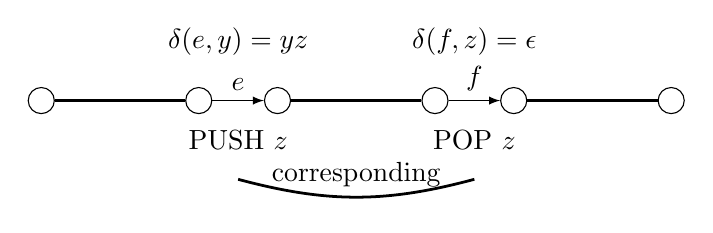
\begin{tikzpicture}
	\begin{pgfonlayer}{nodelayer}
		\node [style=state] (0) at (0, -0) {};
		\node [style=state] (1) at (2, -0) {};
		\node [style=state] (2) at (3, -0) {};
		\node [style=state] (3) at (5, -0) {};
		\node [style=state] (4) at (6, -0) {};
		\node [style=none] (5) at (2.5, 0.75) {$\delta(e, y )= yz$};
		\node [style=none] (6) at (5.5, 0.75) {$\delta(f, z)=\epsilon$};
		\node [style=state] (7) at (8, -0) {};
		\node [style=none] (8) at (2.5, -0.5) {PUSH $z$};
		\node [style=none] (9) at (5.5, -0.5) {POP $z$};
		\node [style=none] (10) at (2.5, -1) {};
		\node [style=none] (11) at (5.5, -1) {};
	\end{pgfonlayer}
	\begin{pgfonlayer}{edgelayer}
		\draw [style=transition] (1) to node[auto]{$e$} (2);
		\draw [style=transition] (3) to node[auto]{$f$} (4);
		\draw [style=simple] (0) to (1);
		\draw [style=simple] (2) to (3);
		\draw [style=simple] (4) to (7);
		\draw [style=simple, bend right=15, looseness=1.00] (10.center) to node[auto]{corresponding} (11.center);
	\end{pgfonlayer}
\end{tikzpicture}
\end{center}

The corresponding path in the graph $G'$:

\begin{center}
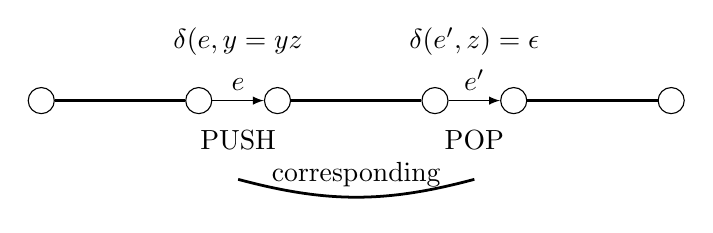
\begin{tikzpicture}
	\begin{pgfonlayer}{nodelayer}
		\node [style=state] (0) at (0, -0) {};
		\node [style=state] (1) at (2, -0) {};
		\node [style=state] (2) at (3, -0) {};
		\node [style=state] (3) at (5, -0) {};
		\node [style=state] (4) at (6, -0) {};
		\node [style=none] (5) at (2.5, 0.75) {$\delta(e, y = yz$};
		\node [style=none] (6) at (5.5, 0.75) {$\delta(e', z)=\epsilon$};
		\node [style=state] (7) at (8, -0) {};
		\node [style=none] (8) at (2.5, -0.5) {PUSH};
		\node [style=none] (9) at (5.5, -0.5) {POP};
		\node [style=none] (10) at (2.5, -1) {};
		\node [style=none] (11) at (5.5, -1) {};
	\end{pgfonlayer}
	\begin{pgfonlayer}{edgelayer}
		\draw [style=transition] (1) to node[auto]{$e$} (2);
		\draw [style=transition] (3) to node[auto]{$e'$} (4);
		\draw [style=simple] (0) to (1);
		\draw [style=simple] (2) to (3);
		\draw [style=simple] (4) to (7);
		\draw [style=simple, bend right=15, looseness=1.00] (10.center) to node[auto]{corresponding} (11.center);
	\end{pgfonlayer}
\end{tikzpicture}
\end{center}

The relation $\rho'$ between the edges of $G'$ can be visualized as a bipartite
graph:

\begin{center}
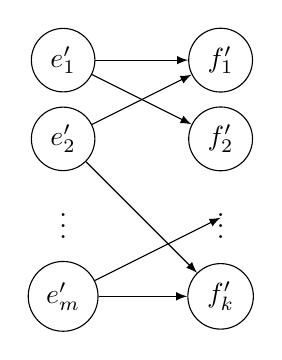
\begin{tikzpicture}
	\begin{pgfonlayer}{nodelayer}
		\node [style=state] (0) at (-1, 2) {$e'_1$};
		\node [style=state] (1) at (-1, 1) {$e'_2$};
		\node [style=state] (2) at (-1, -1) {$e'_m$};
		\node [style=state] (3) at (1, 2) {$f'_1$};
		\node [style=state] (4) at (1, 1) {$f'_2$};
		\node [style=state] (5) at (1, -1) {$f'_k$};
		\node [style=none] (6) at (-1, -0) {$\vdots$};
		\node [style=none] (7) at (1, -0) {$\vdots$};
	\end{pgfonlayer}
	\begin{pgfonlayer}{edgelayer}
		\draw [style=transition] (0) to (3);
		\draw [style=transition] (0) to (4);
		\draw [style=transition] (1) to (3);
		\draw [style=transition] (1) to (5);
		\draw [style=transition] (2) to (5);
		\draw [style=transition] (2) to (7.center);
	\end{pgfonlayer}
\end{tikzpicture}
\end{center}

The edges of this relation connect each edge from $E'$ representing an 
''opening bracket'' (push-operation) with those edges from $E'$
representing the corresponding ''closing bracket'' (pop-operation).

To get a one-to-one relation, the edges of the relation $\rho'$ are multiplied
as needed. The result is a new relation $\tilde{\rho}$ in which each
opening bracket has a unique closing bracket:

\begin{center}
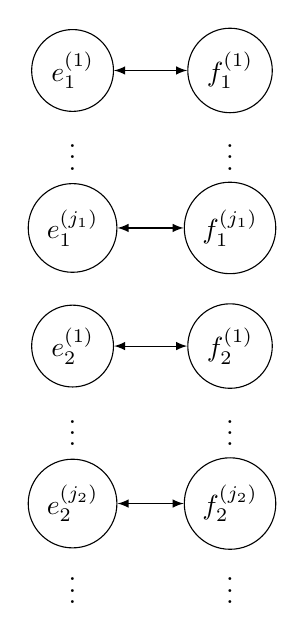
\begin{tikzpicture}
	\begin{pgfonlayer}{nodelayer}
		\node [style=state] (0) at (-1, 3) {$e_1^{(1)}$};
		\node [style=state] (1) at (-1, 1) {$e_1^{(j_1)}$};
		\node [style=state] (2) at (1, 3) {$f_{1}^{(1)}$};
		\node [style=state] (3) at (1, 1) {$f_{1}^{(j_1)}$};
		\node [style=none] (4) at (-1, -3.5) {$\vdots$};
		\node [style=none] (5) at (1, -3.5) {$\vdots$};
		\node [style=state] (6) at (-1, -0.5) {$e_{2}^{(1)}$};
		\node [style=state] (7) at (1, -0.5) {$f_{2}^{(1)}$};
		\node [style=state] (8) at (-1, -2.5) {$e_{2}^{(j_2)}$};
		\node [style=state] (9) at (1, -2.5) {$f_{2}^{(j_2)}$};
		\node [style=none] (10) at (1, -1.5) {$\vdots$};
		\node [style=none] (11) at (-1, -1.5) {$\vdots$};
		\node [style=none] (12) at (1, 2) {$\vdots$};
		\node [style=none] (13) at (-1, 2) {$\vdots$};
	\end{pgfonlayer}
	\begin{pgfonlayer}{edgelayer}
		\draw [style=bijection] (0) to (2);
		\draw [style=bijection] (1) to (3);
		\draw [style=bijection] (6) to (7);
		\draw [style=bijection] (8) to (9);
	\end{pgfonlayer}
\end{tikzpicture}
\end{center}

The edges that have been created by multiplying an edge $e' \in E'$ are called
the {\em parallel edges} of $e'$.

For edges $(\tilde{e}, \tilde f) \in \tilde{\rho}$ we also write $\tilde f =
\inv{\tilde e}$ and call $\tilde f$ the {\em inverse edge} to $\tilde e$.

In the graph $\tilde{G}$ we replace the edges of $G'$ by their parallel edges:

\begin{center}
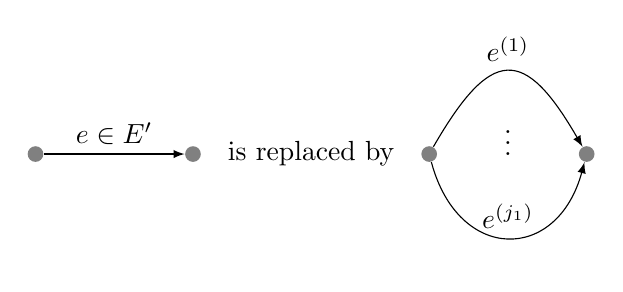
\begin{tikzpicture}
	\begin{pgfonlayer}{nodelayer}
		\node [style={filled_vertex}] (0) at (-5, -0) {};
		\node [style={filled_vertex}] (1) at (-3, -0) {};
		\node [style={filled_vertex}] (2) at (0, -0) {};
		\node [style={filled_vertex}] (3) at (2, -0) {};
		\node [style=none] (4) at (1, 0.25) {$\vdots$};
		\node [style=none] (5) at (-1.5, -0) {is replaced by};
	\end{pgfonlayer}
	\begin{pgfonlayer}{edgelayer}
		\draw [style=transition] (0) to node[auto]{$e \in E'$} (1);
		\draw [style=transition, bend left=60, looseness=2.00] (2) to
		node[auto]{$e^{(1)}$} (3); 
		\draw [style=transition, bend right=75,looseness=1.75] (2) to
		node[auto]{$e^{(j_1)}$} (3);
	\end{pgfonlayer}
\end{tikzpicture}
\end{center}

A parallel edge $e'[i] \in \tilde E$ has the same source and target as
the original edge $e' \in G'$:
\[ Q(e'[i]) = Q(e'),\quad Z(e'[i]) = Z(e') \]

By our construction it holds:
If $(e', f') \in \rho'$ then there exists exactly one pair of parallel edges
$(\tilde e, \tilde f) \in \tilde\rho$ such that $\tilde f = \inv{\tilde e}$.

From $G'$ we construct the graph $\tilde{G} = (\tilde{V}, \tilde{E})$ by setting
\begin{eqnarray*}
\tilde{V} &:=& V' \ (=V \cup \setof{s_0}) \\
\tilde{E} &:=& \setof{\tilde e \mid \tilde e \text{ is parallel edge for
some }e' \in E'}
\end{eqnarray*}

If $\tilde e \in \tilde{E}$ is a parallel edge for some $e' \in E'$ we write:
\[ e' = \proj{\tilde e}\quad (e'\text{ is the projection of }\tilde e \] 

For each path $\tilde{\pi} \in \pathcat{\tilde{G}}$ then holds
$\proj{\tilde{\pi}} \in \pathcat{G'}$, i.e.\ the paths of parallel edges are
projected to paths in $G'$.

\newcommand{\validpaths}{\mathrm{VP}}
We define the set of {\em valid paths} in $\tilde{G}$ by
\begin{eqnarray*}
\validpaths &=& \{ \tilde e_1 \cdots \tilde e_k \in \pathcat{\tilde{G}}
\mid \tilde{e_i} \in \tilde{E} \\
& & \text{and for each pair }(\tilde e_i, \tilde e_{i+1})\text{ of consecutive
edges holds:}\\
& & \gamma(\proj{\tilde{e}_i} \cdot \proj{\tilde{e}_{i+1}}) \not\equiv 0\text{
in the polycyclic monoid }\pocymon{Y} \,\}
\end{eqnarray*}

\newcommand{\acceptedpaths}{\mathrm{VAP}}
We define the set of {\em valid accepted} paths in $\tilde{G}$ by
\begin{equation*}
\acceptedpaths = \setof{\tilde\pi \in \validpaths \mid Q(\tilde\pi) \in
S,\ Z(\tilde\pi) \in F} \subset \validpaths
\end{equation*}

Note that $\validpaths$ and $\acceptedpaths$ both are {\em local} sets.

\medskip
We define the (positive) alphabet $\Sigma$ as the set of those parallel edges
that are projected to edges which execute a push-operation:
\begin{equation*}
\Sigma := \tilde{E}^+ := \setof{\tilde e \in \tilde{E} \mid \proj{\tilde e} =
(e, y) \in E \times Y}
\end{equation*}

Then the edge set of the graph $\tilde{G}$ is divided into $\tilde{E}
= \tilde{E}^+ \cup \tilde{E}^-$.

For the proof of the theorem we need two lemmata.

A path in $\tilde{G}$ is called {\em well-nested} if it can be reduced to the
empty path using the relations 
\[ \tilde{e} \cdot \inv{\tilde{e}} = \epsilon,\quad \tilde{e}, \inv{\tilde{e}}
\in E'\]

(The lemma from the original book has been reformulated.)

\begin{lemma}
If $\tilde{\pi} \in \validpaths$ is a non-empty valid path and $\tilde\pi$ is
well-nested, then for the projection $\pi' = \proj{\tilde{\pi}}$ holds:
\[ |\gamma(\pi')| = y \inv{y}\text{ for some }y \in Y \]
\end{lemma}

\begin{proof}
The proof uses induction over the path length. Observe that a well-nested
path has even length, therefore a well-nested, non-empty path has length at
least two.

Remember the definition of the Dyck language $D(\Sigma)$ over an alphabet
$\Sigma$:
\begin{eqnarray*}
d \in D(\Sigma) &\Rightarrow& \sigma \cdot d \cdot \inv{\sigma} \in
D(\Sigma)\text{ for each }\sigma \in \Sigma \\
d_1, d_2 \in D(\Sigma) &\Rightarrow& d_1 \cdot d_2 \in D(\Sigma)
\end{eqnarray*}

{\em Induction base:} $\len{\tilde{\pi}}=2$
\begin{eqnarray*}
\tilde{\pi} = \tilde e \cdot \inv{\tilde e} &\Rightarrow& (\tilde e, \inv{\tilde
e}) \in \tilde{\rho} \\
&\Rightarrow& (\proj{\tilde e}, \proj{\inv{\tilde e}}) \in \rho'\text{ where }\\
&& \proj{\tilde e} \in E \times Y\text{ is a ''push''-edge and} \\
&& \proj{\inv{\tilde e}} \in E \times Y \times Y_0\text{ is the
corresponding ''pop''-edge}
\end{eqnarray*}

$\proj{\tilde{\pi}} = \proj{\tilde e} \cdot \proj{\inv{\tilde e}}$

If
\begin{eqnarray*}
\gamma(\proj{\tilde e}) &=& \inv{y} y z \qquad\text{(''guess $y$;\ push $z$'')}
\\
\gamma(\proj{\inv{\tilde e}}) &=& \inv{z} \inv{y} y \qquad\text{(''pop $z$;\
guess $y$'')} \\
\text{then} \\
|\gamma(\proj{\tilde{\pi}})| &=& |\gamma(\proj{\tilde e}) \cdot
\gamma(\proj{\inv{\tilde e}})| \\
&=& |\inv{y} y z \cdot \inv{z} \inv{y} y| \\
&=& |\inv{y} y (z \cdot \inv{z}) \inv{y} y| \\
&=& |\inv{y} (y \inv{y}) y| \\
&=& |\inv{y} y| \\
&=& \inv{y} y
\end{eqnarray*}

\medskip
{\em Induction step:}

{\em Case 1:} Let the claim be true for a well-nested path $\tilde{\pi}$. Then
$|\tilde{\pi}| = \epsilon$ and for the projection $\proj{\tilde{\pi}}$ holds
\[ |\gamma(\proj{\tilde{\pi}})| = \inv{y_1} \cdot y_1\text{ for some }y_1 \in Y
\]

Consider the path $\tilde e \cdot \tilde{\pi} \cdot \inv{\tilde e}.$ It is
well-nested because $\tilde\pi$ is well-nested.

For the projection
\[ \proj{\tilde e \cdot \tilde{\pi} \cdot \inv{\tilde e}} = \proj{\tilde e}
\cdot \proj{\tilde{\pi}} \cdot \proj{\inv{\tilde e}} \in \pathcat{G'} \]
where
\begin{eqnarray*}
\proj{\tilde e} &=& (e_1, y) \qquad\text{''push $z$-edge''}\\
\proj{\inv{\tilde e}} &=& (e_2, z, y) \qquad\text{''pop $z$-edge''}\\
\end{eqnarray*}
we get:
\begin{eqnarray*}
|\gamma(\proj{\tilde e} \cdot \proj{\tilde{\pi}} \cdot \proj{\inv{\tilde
e}})|&=& |\gamma(\proj{\tilde e}) \cdot \gamma(\proj{\tilde{\pi}}) \cdot
\gamma(\proj{\inv{\tilde e}})| \\
&=&|\gamma((e_1, y)) \cdot  (\inv{y_1} y_1) \cdot \gamma((e_2, z, y))| \\
&=& |(\inv{y} \cdot y \cdot z) \cdot (\inv{y_1} \cdot y_1) \cdot (\inv{z} \cdot
\inv{y} \cdot y)| \\
\end{eqnarray*}
Because $\tilde e \cdot \tilde{\pi} \cdot \inv{\tilde e}$ is well-nested it
must hold $z = y_1$. Otherwise from $z \cdot \inv{y_1} \equiv 0$ would
follows $e \cdot \tilde{\pi} \cdot \inv{e} \equiv 0$ which would be a 
contradiction to our assumptions.

Therefore
\begin{eqnarray*}
|(\inv{y} \cdot y \cdot z) \cdot (\inv{y_1} \cdot y_1) \cdot (\inv{z} \cdot
\inv{y} \cdot y)| &=&
|(\inv{y} \cdot y \cdot z) \cdot (\inv{z} \cdot z) \cdot (\inv{z} \cdot
\inv{y} \cdot y)| \\
&=& |\inv{y} \cdot (y \cdot (z \cdot \inv{z}) \cdot (z \cdot \inv{z}) \cdot
\inv{y}) \cdot y| \\
&=& |\inv{y} \cdot (y \cdot \inv{y}) \cdot y| \\
&=& |\inv{y} \cdot y| \\
&=& \inv{y}  \cdot y
\end{eqnarray*}

\medskip
{\em Case 2:} Let $\tilde{\pi} = \tilde{\pi}_1 \cdot \tilde{\pi}_2$ be a valid
path which is the product of two well-nested paths, i.e.\ $|\tilde{\pi}_1| =
|\tilde{\pi}_2| = \epsilon$.

Consider
\begin{eqnarray*}
|\gamma(\proj{\tilde{\pi}})| &=& |\gamma(\proj{\tilde{\pi}_1 \cdot
\tilde{\pi}_2})| \\
&=& |\gamma(\proj{\tilde{\pi}_1}) \cdot \gamma(\proj{\tilde{\pi}_2})| \\
&=& (\inv{y_1} \cdot y_1) \cdot (\inv{y_2} \cdot y_2),\text{ for some }y_1, y_2
\in Y\text{ by induction hypothesis}
\end{eqnarray*}

Because $\tilde{\pi}_1 \cdot \tilde{\pi}_2$ is valid, it must hold $y_1 = y_2$.
Otherwise it would be $y_1 \cdot \inv{y_2} \equiv 0$ which would violate our 
assumptions.

Therefore we get
\begin{eqnarray*}
|\gamma(\proj{\tilde{\pi}})| &=& (\inv{y_1} \cdot y_1) \cdot (\inv{y_2} \cdot
y_2)\\
&=& \inv{y_1} \cdot y_1 \cdot \inv{y_1} \cdot y_1 \\
&=& \inv{y_1} \cdot y_1
\end{eqnarray*}
\end{proof}

The lemma of course also holds for well-nested {\em accepted paths}. For the
projection of such a path $\tilde\pi \in \acceptedpaths,\ \tilde\pi \equiv
\epsilon$,  holds 
\[ \pi = \proj{\tilde{\pi}} \in \pathcat{G'}(S, F) \Rightarrow |\gamma(\pi)| =
\inv{y_0} y_0 \]
where $y_0$ is the special symbol in the pushdown alphabet.

\bigskip
\begin{lemma}
For each path $\pi' \in \pathcat{G'}$ with
\[ |\gamma(\pi')| = \inv{y} y \quad\text{for some }y \in Y \]
there exists exactly one path $\tilde{\pi} \in \validpaths$ with 
\[ |\tilde{\pi}| = \epsilon\text{ and }\pi' = \proj{\tilde{\pi}} \] 
\end{lemma}

\begin{proof}
TODO
\end{proof}

Similar as after lemma 1 one can conclude here that for each path $\pi' \in
\pathcat{G'}(S, F)$ with $|\gamma(\pi')| = \inv{y_0} y_0$ there exists exactly
one well-nested path $\tilde{\pi} \in \acceptedpaths$ with $\proj{\tilde{\pi}} =
\pi'$ and $|\tilde{\pi}| = \epsilon$.

\medskip
Using both lemmata we can now prove the theorem:
\begin{eqnarray*}
L_\kappa &=& \setof{\alpha(\pi) \mid \pi \in \pathcat{G}(S, F),\ \delta(\pi,
\epsilon) = \epsilon}\text{ (by definition of PDA)} \\
&=& \setof{\alpha(\pi') \mid \pi' \in \pathcat{G'}(s_0, F),\ |\gamma(\pi')| =
y_0}\text{ (by theorem 2, chapter III.1)} \\
&=& \setof{\alpha(\pi') \mid \pi' \in \pathcat{G'}(S, F),\
|\gamma(\pi')| = \inv{y_0} y_0}\text{ (by construction of $G'$)}
\end{eqnarray*}

If we define $R := \acceptedpaths$, we get $R \in \reglang(\unioninv{\Sigma})^*$
because every local language is regular.

Together with lemma 1 and lemma 2 it follows
\[ \proj{R \cap D(\underbrace{\tilde{E}^+}_{\Sigma})} = \setof{\pi' \in
\pathcat{G'}(s_0, F) \mid |\gamma(\pi')| = y_0} \]

With the homomorphism
\[ \phi := (\mathbf{p} \circ \alpha) : (\unioninv{\Sigma})^* \to X^* \]
we get
\[ L_\kappa = \phi(D(\Sigma) \cap R) \]
\end{proof}

We even proved slightly more: Let 
\[ {<}\kappa, w{>} := \card{\setof{\pi \in
\pathcat{G}(S,F) \mid \alpha(\pi) = w,\ \delta(\pi, \epsilon) = \epsilon}}
\]
be the number of accepting computations of the PDA $\kappa$ for the word $w$.

\begin{corollary}
For each PDA $\kappa$ there exists a Dyck language $D(\Sigma)$ and a local set
$R$ over $\unioninv{\Sigma}$ and a monoid homomorphism $\phi:
(\unioninv{\Sigma})^* \to X^*$ such that
\begin{enumerate}
  \item $\phi(D(\Sigma\cap R)) = L_\kappa$
  \item For $w\in X^*$ it holds ${<}\kappa, w{>} = \card{\phi^{-1}(w)}$
\end{enumerate}
\end{corollary}

\begin{proof}\ 

\begin{enumerate}
  \item Chomsky-Schützenberger theorem
  \item Follows from the construction in the proof. (The inverse homomorphism
  gives the different accepting computations for a word.)
\end{enumerate}
\end{proof}

Problem: Is it possible to always find a PDA $\kappa$ accepting 
$L \in \alglang(X^*)$ such that for each word $w$ it holds 
${<}\kappa, w{>} < \infty$?

If the definition of the pushdown store is generalized such that $\delta(X
\times Y) \subset Y^*$ is allowed, is then the condition ${<}\kappa, w{>} <
\infty$ always satisfiable?

This problem will be investigated in a later chapter.

\medskip
At the end of this section, for interested readers we want to mention the
following:

The Dyck language $D(X) \in \alglang(X_\infty^*)$ is algebraic.

By theorem 1 in section III.2 it holds that the class of algebraic languages is
closed under monoid homomorphism, and by theorem 3 in chapter III.2 also closed
under intersection with regular sets.

From the Chomsky-Schützenberger theorem therefore follows that the class of
algebraic languages over the alphabet $X_\infty$ is exactly the class of
context-free languages.

\section{The finite automaton with storage}

In the following we slightly modify the notion of a pushdown-store by admitting
arbitrary monoids instead of the free monoid $Y^*$.

Doing so, the given definition of the pushdown-store cannot be used any longer
because for arbitrary monoids the notion of a ''topmost'' factor cannot be
defined in a meaningful way.

In our finite automaton with storage the control unit puts symbols onto the
store without caring about its current content which gives an even stronger
separation between control unit and pushdown-store as we had for pushwon
automata.

With the finite automaton with storage we have a universal model of automata.

\begin{definition}
$\fa{P} = (\fa{A}, \store{P})$ is called {\bf finite automaton with storage}
$\iff$
\begin{eqnarray*}
& \fa{A}=(G, X, S, F, \alpha),\ (G=(V,E),\text{ is a finite automaton} \\
& \fa{P}=(E, M, D, C, \gamma)\text{ is a storage with monoid }M \\
& \gamma: E^* \to M\text{ is a monoidhomomorphism} \\
& D,C \subset M\text{ ($D$=domain, $C$= codomain)}
\end{eqnarray*}
\end{definition}

\[ L_{\fa{P}} = \setof{\alpha(\pi) \mid \pi \in \pathcat{G}(S, F),\ D\cdot
\gamma(\pi) \cap C \neq \emptyset}
\]
is the {\bf language accepted by} $\fa{P}$.

Remark: In the following we will also just write ''finite automaton with storage
monoid $M$'' if this does not lead to any misunderstandings.

\bigskip
The following theorem gives a relation between the pushdown automaton and the
finite automaton with storage.

\begin{theorem}
If $\kappa = (\fa{A}, \store{K})$ is a pushdown automaton, then there exists a
finite automaton with storage $\fa{P}$ with storage monoid $\hgroup{Y}$ such
that $L_{\kappa} = L_{\fa{P}}$.
\end{theorem}

\begin{proof}
We remember the proof of the Chomsky-Schützenberger theorem in the previous
section.

Let
\[ \fa{A}'=(G', \hgroup{Y}, S_0, F, \gamma),\ G'=(V',E') \]
be the finite automaton used in the proof with accepted language
\[ L_\kappa = \setof{\alpha(\pi) \mid \pi \in \pathcat{G'}(S_0,F),\
|\gamma(\pi)|=y_0} \]

We set
\[ M := \hgroup{Y},\qquad E' \to \hgroup{Y} \]

Then for the automaton with storage $\fa{P}=(\fa{A}, \store{P})$ with 
\[ \store{P} = (E', \hgroup{Y}, \setof{\epsilon}, \setof{y_0}, \gamma) \]
it holds $L_\kappa = L_{\fa{P}}$.
\end{proof}

\bigskip
It is now possible to prove similar closure properties for our new type of
automaton as we did before for pushdown automata, in the corresponding
constructions one has to complement these for the used monoids.

We do not want to execute these constructions here.

\bigskip
\begin{theorem}[]
Let $\fa{P}=(\fa{A}, \store{P})$ be a finite automaton with storage monoid
$\pocymon{Y},\ C = D = \setof{\epsilon}$. Then there exists a pushdown automaton
$\kappa = (\fa{A}, \store{K})$ with $L_{\fa{P}} = L_\kappa$.
\end{theorem}

\begin{proof}
Let $\fa{P}=(\fa{A}, \store{P})$ with
\[ \fa{A}=(G, X, S, F, \alpha),\ G=(V,E),\quad \store{P}=(E, \pocymon{Y},
\setof{\epsilon}, \setof{\epsilon}, \gamma) \]

Without loss of generality let $\gamma(e) \in Y \cup Y^{-1} \cup
\setof{\epsilon}$ (this can be achieved by breaking the graph edges).

We define the pushdown automaton $\kappa = (\fa{A}, \store{K})$ as follows:
\[ \store{K} = (E, Y_1^*, \delta)\text{ with }Y_1 = Y \cup \setof{0} \]

The pushdown computation $\delta$ is 
\[ \delta: E \times Y_1 \to (Y_1 \times Y_1) \cup Y_1 \cup \setof{\epsilon} \]
defined by
\[ \delta(e, y) = \begin{cases}
	|y \cdot \gamma(e)| & \text{if }\gamma(e) \in Y \cup \setof{\epsilon}\text{ or
	} \gamma(e) = y^{-1} \\
	y \cdot 0 & \text{else}
\end{cases} \]

Claim: $L_\kappa \stackrel{!}{=} L_{\fa{P}}$

''$\supset$'': Let $w \in L_{\fa{P}}$, then there exists a path $\pi \in
\pathcat{G}(S, F)$ with label $\alpha(\pi) = w$ and storage computation
$\gamma(\pi) = \epsilon$ and for each prefix path $\pi'$ of $\pi$ holds:
\[ |\gamma(\pi')| = \delta(\pi', \epsilon) \]
This is easily proved by induction and left to the reader.

Therefore $w \in L_\kappa$.

\bigskip
''$\subset$'': Let $w \in L_\kappa$, then there exists a path $\pi \in
\pathcat{G(S, F)}$ with label $\alpha(\pi)=w$ and pushdown computation
$\delta(\pi, \epsilon) = \epsilon$.

Wit part 1 the claim holds again from which follows $w \in L_{\fa{P}}$.

From both parts follows the claim.
\end{proof}

\bigskip
Remark: The theorem also holds if we use the H-group $\hgroup{X}$ as storage
monoid (exercise).

From theorem 1 and theorem 2 it follows the equivalence of the automata models
with storage monoid $\hgroup{X}$.

\bigskip
As an example we give a finite automaton with storage which accepts the language
$L$ over the alphabet $X = \setof{a, b, c}$ defined as follows:
\begin{enumerate}
  \item $d \in L$
  \item $x, y \in L \Rightarrow a\cdot x\cdot b\cdot y\cdot c\in L$
  \item $L$ is minimal with 1) and 2)
\end{enumerate}

$L$ can be understood as the language of the bracketed arithmetic expressions.

We create the following preliminary (infinite) graph $G$ for $L$:

\begin{center}
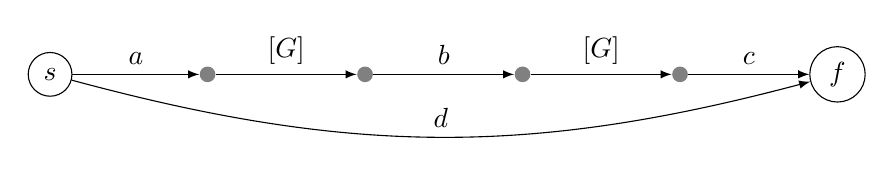
\begin{tikzpicture}
	\begin{pgfonlayer}{nodelayer}
		\node [style=state] (0) at (0, -0) {$s$};
		\node [style={filled_vertex}] (1) at (2, -0) {};
		\node [style={filled_vertex}] (2) at (4, -0) {};
		\node [style={filled_vertex}] (3) at (6, -0) {};
		\node [style={filled_vertex}] (4) at (8, -0) {};
		\node [style=state] (5) at (10, -0) {$f$};
	\end{pgfonlayer}
	\begin{pgfonlayer}{edgelayer}
		\draw [style=transition] (0) to node[auto]{$a$} (1);
		\draw [style=transition] (1) to node[auto]{$[G]$} (2);
		\draw [style=transition] (2) to node[auto]{$b$} (3);
		\draw [style=transition] (3) to node[auto]{$[G]$} (4);
		\draw [style=transition] (4) to node[auto]{$c$} (5);
		\draw [style=transition, bend right=15, looseness=1.00] (0) to node[auto]{$d$} (5);
	\end{pgfonlayer}
\end{tikzpicture}
\end{center}

We want to remove each edge labeled with $[G]$ by adding an $\epsilon$-edge
from the source of this edge to $s$ and from $f$ to the target of the $[G]$-
edges.

We get the following graph $G'$:

\begin{center}
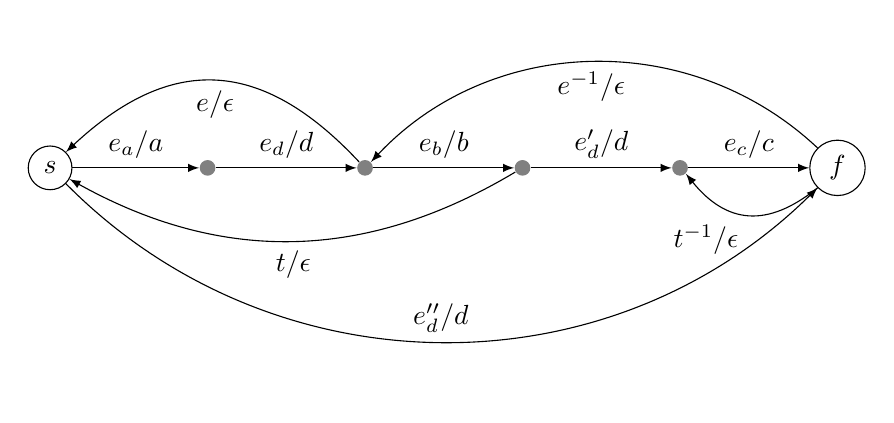
\begin{tikzpicture}
	\begin{pgfonlayer}{nodelayer}
		\node [style=state] (0) at (0, -0) {$s$};
		\node [style={filled_vertex}] (1) at (2, -0) {};
		\node [style={filled_vertex}] (2) at (4, -0) {};
		\node [style={filled_vertex}] (3) at (6, -0) {};
		\node [style={filled_vertex}] (4) at (8, -0) {};
		\node [style=state] (5) at (10, -0) {$f$};
	\end{pgfonlayer}
	\begin{pgfonlayer}{edgelayer}
		\draw [style=transition] (0) to node[auto]{$e_a/a$} (1);
		\draw [style=transition] (1) to node[auto]{$e_d/d$} (2);
		\draw [style=transition] (2) to node[auto]{$e_b/b$} (3);
		\draw [style=transition] (3) to node[auto]{$e'_d/d$} (4);
		\draw [style=transition] (4) to node[auto]{$e_c/c$} (5);
		\draw [style=transition, bend right=45, looseness=1.00] (0) to node[auto]{$e''_d/d$} (5);
		\draw [style=transition, bend right=45, looseness=1.25] (2) to node[auto]{$e/\epsilon$} (0);
		\draw [style=transition, bend right=45, looseness=1.00] (5) to node[auto]{$e^{-1}/\epsilon$} (2);
		\draw [style=transition, bend left=45, looseness=1.25] (5) to node[auto]{$t^{-1}/\epsilon$} (4);
		\draw [style=transition, bend left, looseness=1.00] (3) to node[auto]{$t/\epsilon$} (0);
	\end{pgfonlayer}
\end{tikzpicture}
\end{center}

The graph $G'=(V',E')$ is finite but the corresponding finite acceptor would
also accept words which are not elements of $L$. This has to be corrected by 
defining a suitable storage.

Define $\gamma: E' \to \pocymon{\setof{a, b, s, t}}$ by
\begin{eqnarray*}
\gamma(e_a) & = & a \\
\gamma(e) & = & s \\
\gamma(e_d) & = & \epsilon \\
\gamma(t) & = & t \\
\gamma(e_b) & = & a^{-1} \cdot b \\
\gamma(e_c) & = & b^{-1} \\
\gamma(e'_d) & = & \epsilon \\
\gamma(e''_d) & = & \epsilon \\
\gamma(e^{-1}) & = & s^{-1} \\
\gamma(t^{-1}) & = & t^{-1} \\
\end{eqnarray*}

Domain and codomain contain the empty word only, the storage monoid $M$ is the
H-group over $X$:
\[ D = C = \setof{\epsilon},\quad M = \hgroup{\setof{a, b, s, t}} \]

For
\[ \fa{A} = (G', \setof{a, b,c d}, \setof{s}, \setof{f}, \alpha) \]
and storage 
\[ \store{P} = (E', M, D, C, \gamma) \]
the finite automaton with storage $\fa{P} = (\fa{A}, \store{P})$ accepts L:
\[ L_{\fa{P}} = \setof{\alpha(\pi) \mid \pi \in \pathcat{G'}(s, f),\ D \cdot
\gamma(\pi) \cap C \neq \emptyset} = L \]

Proof: exercise.

Now we want to remove the $\epsilon$-edges from the graph $G'$. To do so, we use
the algorithm from chapter II, lemma 2 and get:

\begin{center}
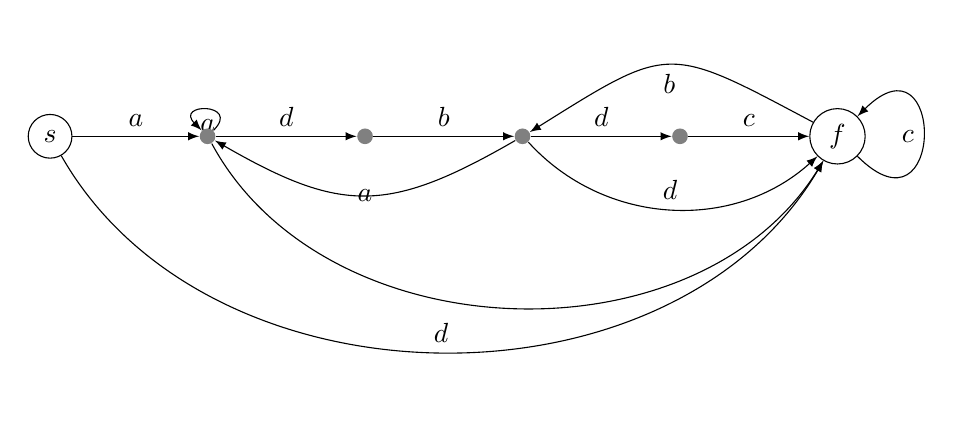
\begin{tikzpicture}
	\begin{pgfonlayer}{nodelayer}
		\node [style=state] (0) at (0, -0) {$s$};
		\node [style={filled_vertex}] (1) at (2, -0) {};
		\node [style={filled_vertex}] (2) at (4, -0) {};
		\node [style={filled_vertex}] (3) at (6, -0) {};
		\node [style={filled_vertex}] (4) at (8, -0) {};
		\node [style=state] (5) at (10, -0) {$f$};
	\end{pgfonlayer}
	\begin{pgfonlayer}{edgelayer}
		\draw [style=transition] (0) to node[auto]{$a$} (1);
		\draw [style=transition] (1) to node[auto]{$d$} (2);
		\draw [style=transition] (2) to node[auto]{$b$} (3);
		\draw [style=transition] (3) to node[auto]{$d$} (4);
		\draw [style=transition] (4) to node[auto]{$c$} (5);
		\draw [style=transition, bend right=60, looseness=1.00] (0) to node[auto]{$d$} (5);
		\draw [style=transition, in=135, out=45, loop] (1) to node[auto]{$a$} ();
		\draw [style=transition, in=45, out=-45, loop] (5) to node[auto]{$c$} ();
		\draw [style=transition, bend left, looseness=1.25] (3) to node{$a$} (1);
		\draw [style=transition, bend right=60, looseness=1.00] (1) to (5);
		\draw [style=transition, bend right=45, looseness=1.00] (3) to node[auto]{$d$} (5);
		\draw [style=transition, bend right, looseness=1.50] (5) to node[auto]{$b$} (3);
	\end{pgfonlayer}
\end{tikzpicture}
\end{center}

The storage is given by

\begin{center}
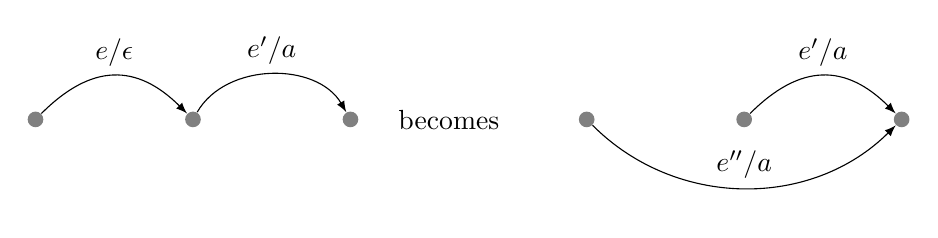
\begin{tikzpicture}
	\begin{pgfonlayer}{nodelayer}
		\node [style={filled_vertex}] (0) at (0, -0) {};
		\node [style={filled_vertex}] (1) at (2, -0) {};
		\node [style={filled_vertex}] (2) at (4, -0) {};
		\node [style={filled_vertex}] (3) at (7, -0) {};
		\node [style={filled_vertex}] (4) at (9, -0) {};
		\node [style={filled_vertex}] (5) at (11, -0) {};
		\node [style=none] (6) at (5.25, -0) {becomes};
	\end{pgfonlayer}
	\begin{pgfonlayer}{edgelayer}
		\draw [style=transition, bend left=45, looseness=1.25] (0) to node[auto]{$e/\epsilon$} (1);
		\draw [style=transition, bend left=60, looseness=1.00] (1) to node[auto]{$e'/a$} (2);
		\draw [style=transition, bend left=45, looseness=1.25] (4) to node[auto]{$e'/a$} (5);
		\draw [style=transition, bend right=45, looseness=1.00] (3) to node[auto]{$e''/a$} (5);
	\end{pgfonlayer}
\end{tikzpicture}
\end{center}

We can simplify the graph even further and get

\begin{center}
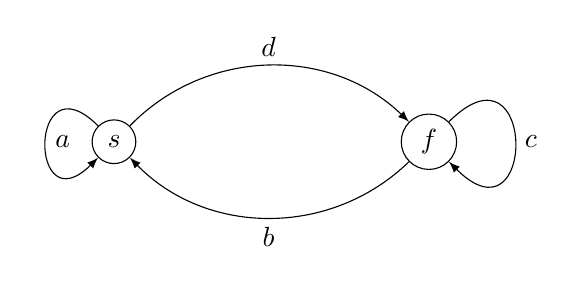
\begin{tikzpicture}
	\begin{pgfonlayer}{nodelayer}
		\node [style=state] (0) at (0, -0) {$s$};
		\node [style=state] (1) at (4, -0) {$f$};
	\end{pgfonlayer}
	\begin{pgfonlayer}{edgelayer}
		\draw [style=transition, bend left=45, looseness=1.00] (0) to node[auto]{$d$} (1);
		\draw [style=transition, bend left=45, looseness=1.00] (1) to node[auto]{$b$} (0);
		\draw [style=transition, in=-135, out=135, loop] (0) to node[auto]{$a$} ();
		\draw [style=transition, in=-45, out=45, loop] (1) to node[auto]{$c$} ();
	\end{pgfonlayer}
\end{tikzpicture}
\end{center}

This graph is deterministic and the storage has the following form:
\[ \gamma(e_a) = a,\ \gamma(e_d) = \epsilon,\ \gamma(e_b) = a^{-1} b,\
\gamma(e_c) = b^{-1} \]

\bigskip
We want to look at an example motivated by practical applications: we define
parts of the syntax of the PASCAL programming language using finite automata
with storage.

Every programming language is based on some vocabular. Programs are constructed
by linear composition of these basic symbols in a way defined by the syntax
rules.

The syntax rules are formulated such that is is easy to verify if a sequence of
basic symbols is legal.

The syntax rules are most often (with advantage over other ways) represented by
flow diagrams which are called {\em syntax diagrams}.

The possible paths in these syntax diagrams represent all possible symbol
sequences.

Starting with a diagram labeled ''program'', along the path one either switches
to another diagram if a rectangle is met, one appends a basic symbol $w$ to the
program text if a circle labelled with $w$ is met. A complete example for this
kind of syntac definition can be found in \cite{Wirth}.

We will present syntax diagrams slightly different. We use kind of a dual graph
by making the vertices of the syntax diagrams to edges of our graphs.

In the following example we always show first the syntax diagram as given in
\cite{Wirth} and afterwards show the graph of our finite automaton with storage
that accepts the language defined by the syntax diagram.

\missingfigure

Remark: A program in PASCAL by this definition is a block followed by a dot.

\missingfigure

[Block] may be interpreted as a procedure call of a procedure ''Block''
(corresponds to the substitution of chapter III.2).

Storage:
\[ \gamma(e_1) = s,\quad \gamma(e_2) = s^{-1},\qquad D = C = \setof{\epsilon} \]

In this very simple example no difficulties arise. We want to consider now a
diagram in which the same diagram's name occurs again. This corresponds to a
recursive procedure call. We have to copy the diagram at this location.

\missingfigure

This is the syntax diagram which describes a ''block'' in PASCAL. It consists of
a declaration section and a statement section where the declaration section may
be empty.

$G_{\text{block}}$ is shown below:

\missingfigure

For simplicity the nonterminal symbols are shortened to single characters.

$e$ and $e^{-1}$ are edges inverse to each other. In the storage we have to
take care that the nesting depth of the block is correct. The edge $e$ takes
care that in a function or procedure-declaration the body appears correctly and
in case of multiple nesting the end of the block is always correct.

In the way we described now every syntax diagram can be tranlated to a finite
automaton with storage.

For each edge whose label is enclosed by the brackets [ ] there exists a finite
automaton with storage accepting the language associated with the edge.

By substitution of these graphs into the original graph we can then produce
graphs without bracket labels.

With this construction we could construct a finite automaton wit storage for the
complete syntax of the PASCAL programming language that accepts the
syntactically correct PASCAL programs. We get exactly the syntactically correct
programs as the labels of paths in our graph which additionally fulfill the
codomain-condition of the storage.

By the insertion of $\epsilon$-edges when resolving the recursion the automaton
becomes non-deterministic.

In the next section we want to transform the non-deterministic finite automaton
with storage into a deterministic one.

\bigskip
\begin{exercise}
Given the alphabet $X_k = \setof{a_1, \ldots, a_K}$ and the language $L_k :=
\setof{a_1, \ldots, a_k}^{4^k}$.

Define a finite automaton with storage accepting $L_k$ and prove its
correctness.
\end{exercise}

\bigskip
\begin{exercise}
Let $X = \setof{(, ), [, ], \$, c},\ d \notin X$.
\begin{eqnarray*}
L_0 &=& \setof{\epsilon} \\
&\cup& \{x_1 c y_1 c z_1 d \cdots d x_n c y_n c
z_n d \mid n \geq 1,\ y_1 \cdots y_n \in \$ D_2 \\
& & x_i, z_i \in X^*,\ i=1, \ldots, n \} 
\end{eqnarray*}
is called the {\em Greibach language}. ($D_2$ denotes the Dynck language over
\setof{(, ), [, ]}).

Show: There exists a finite automaton with storage accepting $L_0$.
\end{exercise}
















































\section{The deterministic finite automaton with storage}

In this section we will prove a very important theorem about the relation
between non-determinism and determinism of finite automata with storage.

To be able to construct the deterministic automaton we need some definitions.

\begin{definition}
A finite automaton with storage $\fa{P}=(\fa{A},\storage{P})$ is called
\begin{itemize}
  \item {\bf $\epsilon$-free} if $\fa{A}$ is $\epsilon$-free,
  \item {\bf deterministic} if $\fa{A}$ is deterministic,
  \item {\bf complete} if $\fa{A}$ is complete.
\end{itemize}
\end{definition}

\bigskip
\begin{definition}
$(S, +, \cdot, 0, 1)$ is called a {\bf semi-ring} if
\begin{enumerate}
  \item $(S, +, 0)$ is a commutative monoid
  \item $(S, \cdot, 1)$ is a monoid
  \item The distributive laws hold:
  \begin{eqnarray*}
  a \cdot (b + c) &=& a \cdot b + a \cdot c\\
  (a + b) \cdot c &=& a \cdot c + b \cdot c\\
  \end{eqnarray*}
  \item $0 \cdot a = a \cdot 0 = 0$ for all $a \in S$
\end{enumerate}
\end{definition}

\bigskip
\begin{definition}
Let $M$ be a monoid and $S$ a semi-ring.
\[ S(M) := \setof{\lambda: M \to S \mid \card{\setof{m \mid \lambda(m) \neq 0}}
< \infty} \]
is called the {\bf monoid-ring} of the monoid $M$ over the semi-ring $S$.
\end{definition}

Addition and multiplication on $S(M)$ are defined as follows: For $\lambda_1,
\lambda_2 \in S(M)$
\begin{eqnarray*}
(\lambda_1 + \lambda_2)(m) &=& \lambda_1(m) + \lambda_2(m) \\
(\lambda_1 \cdot \lambda_2)(m) &=& \sum_{m_1 \cdot m_2 = m} 
\lambda_1(m) \cdot \lambda_2(m)
\end{eqnarray*}

One can see that $(S(M), +, \cdot)$ again is a semi-ring. We also write
\[ \lambda := \sum_{\substack{m \in M\\\lambda(m)\neq 0}} m \cdot \lambda(m) \]
or also
\[ \sum_{\substack{m \in M\\\lambda(m)\neq 0}} m \cdot {<}\lambda, m{>} \]

The operations are defined in a way that one can calculate with these
expressions as usual.

In the following we will most often consider the semi-ring $S = \mathbb{B}$, the
{\bf Boolean semi-ring}.

\bigskip
Before proving our main theorem we will show some other results on finite
automata with storage.

\bigskip
First we want to give a representation for graphs in the polycyclic monoid
$\pocymon{Y}$.

Let $G=(V, E)$ be a finite graph with $\card{E} = n$, let $\card{Y} = 2$ and
$2^k \geq n$.

Let $\beta: V \to Y^*$ be an injective mapping and let $\strlen{\beta(v)} = k$
for each vertex $v \in V$.

Further let $G' = (\setof{v_0}, E')$ be a single-vertex graph and $\phi: E \to
E'$ a bijection on the edges, and let $Q(e') = Z(e') = v_0$ for each edge $e'
\in E'$.

The mapping $\phi$ can be uniquely continued to a functor $\phi : \pathcat{G}
\to \pathcat{G'}$. As a functor, $\phi$ is also injective.

We complement $G'$ by a storage $\gamma: E' \to \pocymon{Y}$ by setting
\[ \gamma(e') := u^{-1} \cdot v\text{ where }u = \beta(Q(\phi^{-1}(e')))\text{
and }v = \beta(Z(\phi^{-1}(e'))) \]

In this way the storage ''characterizes'' the paths $\phi(\pathcat{G})$.

Obviously it then holds
\begin{lemma}
\begin{eqnarray*}
\pi \in \phi(\pathcat{G}) &\Leftrightarrow& \gamma(\pi) \neq 0 \\
\gamma(\pi) \neq 0 &\Rightarrow& \gamma(\pi) = u^{-1} \cdot v \\
&& \text{with }u = \beta(Q(\phi^{-1}(e'))) \\
&& \text{and }v = \beta(Z(\phi^{-1}(e'))) \\
&& \text{and }\pi = e'_1 \circ \pi' \circ e'_k
\end{eqnarray*}
\end{lemma}

\begin{proof}
''$\Rightarrow$'':

Let $\pi \in \pathcat{G}$ be a path, $\pi = e'_1 \ldots e'_k \Rightarrow Z(e'_i)
= Q(e'_{i+1})$.

There exists a path $\psi \in \pathcat{G}$ such that $\psi = e_1 \ldots e_k$
with $\phi(\psi) = \pi$.
\begin{eqnarray*}
&\Rightarrow& \beta(Z(\phi^{-1}(e'_i))) = \beta(Q(\phi^{-1}(e'_{i+1}))) \\
&\Rightarrow& \beta(Z(\phi^{-1}(e'_i)))^{-1} \cdot \beta(Q(\phi^{-1}(e'_{i+1})))
= 1 \\
&\Rightarrow& \gamma(e'_1 \ldots e'_k) = \beta(Q(\phi^{-1}(e'_1)))^{-1} \cdot
\beta(Z(\phi^{-1}(e'_k)))
\end{eqnarray*}

''$\Leftarrow$'':

Let $\pi \notin \phi(\pathcat{G}),\ \pi = e'_1 \ldots e'_k$ and there exists an
index $i$ such that $Z(\phi^{-1}(e'_i)) \neq Q(\phi^{-1}(e'_{i+1}))$
\begin{eqnarray*}
&\Rightarrow& \beta(Z(\phi^{-1}(e'_i))) \neq \beta(Q(\phi^{-1}(s'_{i+1}))) \\
&\Rightarrow& \beta(Z(\phi^{-1}(s'_i)))^{-1} \cdot \beta(Q(\phi^{-1}(e'_{i+1})))
= 0
\end{eqnarray*}
\end{proof}

We want to clarify the construction using an example. Let $G = (V, E)$ be the
following graph:

\begin{center}
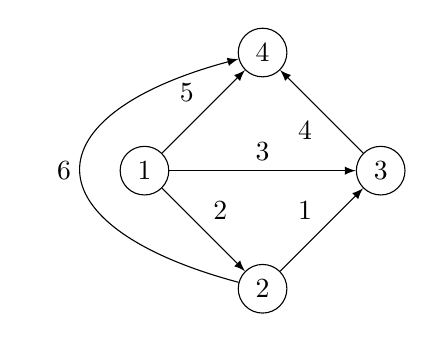
\begin{tikzpicture}
	\begin{pgfonlayer}{nodelayer}
		\node [style=state] (0) at (-1.5, -0) {$1$};
		\node [style=state] (1) at (1.5, -0) {$3$};
		\node [style=state] (2) at (0, 1.5) {$4$};
		\node [style=state] (3) at (0, -1.5) {$2$};
	\end{pgfonlayer}
	\begin{pgfonlayer}{edgelayer}
		\draw [style=transition] (0) to node[auto]{$3$} (1);
		\draw [style=transition] (1) to node[auto]{$4$} (2);
		\draw [style=transition] (0) to node[auto]{$5$} (2);
		\draw [style=transition] (0) to node[auto]{$2$} (3);
		\draw [style=transition] (3) to node[auto]{$1$} (1);
		\draw [style=transition, bend left=75, looseness=2.50] (3) to node[auto]{$6$} (2);
	\end{pgfonlayer}
\end{tikzpicture}
\end{center}

It is $\card{V} = 4 \Rightarrow k = 2\ (= \log_2(4))$.

The mapping $\beta: V \to Y^*,\ Y = \setof{(, [}$ shall be defined by
\[ \beta(1) = [[,\quad \beta(2) = [(,\quad \beta(3) = ([,\quad \beta(4) = (( \]

Let $\phi : E \to E'$ be a bijection and $\gamma: E' \to \pocymon{Y}$ with for
example $\gamma(1) = )]([$.

As a consequence to our construction we get

\begin{theorem}
For each regular language $L \in \reglang(X^*)$ there exists a homomorphism $h:
X^* \to \mathbb{B}(\pocymon{Y})$ with
\[ L = h^{-1}(u^{-1} \cdot v + \sum),\quad \sum \text{ finite sum in
}\mathbb{B}(\pocymon{Y}) \]
$h(x),\ x\in X$ contains only monomials of length $2 \cdot \log_2(n)$ where $n
= \card{V}$.
\end{theorem}

\begin{proof}
$L \in \reglang(X^*)$, then there exists a deterministic finite automaton
\[ \fa{A} = (G, X, S, F, \alpha) \]
with $\card{S} = \card{F} = 1$ which accepts $L$.

To $G = (V, E)$ we construct the single-vertex graph $G' = (V', E')$ and the
mapping $\phi:
E \to E'$ as above. The labelling $\alpha$ is carried over to $E'$ by the
bijection $\phi$. $\gamma$ shall also be defined as above.

We merge all edges with the same label into a single edge $e'$ an define
\[ \gamma'(e') := \sum_{s} \gamma(s) \quad\text{the edges $e$ have the same
label and are merged to $s'$} \]
and continue $\gamma'$ to a homomorphism.

We define our homomorphism $h$ as
\[ h: X^* \to \mathbb{B}(\pocymon{Y})\text{ defined by }h(x) := \gamma'(e'),\
\alpha'(e') = x \]

Then it holds: $w \in L_{\fa{A}} \Leftrightarrow h(w) = u^{-1} \cdot v + \sum$
with $u = \beta(S)$ and $v = \beta(F)$ (exercise) and the length-condition is
also fulfilled.
\end{proof}

\bigskip
We want to use now our graph embedding construction to transform special finite
automata with storage and to approach our goal, the deterministic finite
automaton with storage.

\begin{theorem}
Let $\fa{P} = (\fa{A}, \storage{P})$ be an $\epsilon$-free automaton with
storage monoid $\pocymon{Y}$, let the domain and co-domain be given by $D = C
= \setof{\epsilon}$.

Then there exists a deterministic finite automaton $\fa{P}' = (\fa{A}', \storage{P}')$
with storage $\mathbb{B}(\pocymon{Y})$ (if $\card{Y} \geq 2$) and with
\[ D' = \setof{\epsilon},\qquad C' = \setof{\beta(s)^{-1} \cdot \beta(f) +
\mathbb{B}(\pocymon{Y}) \mid s\in S,\ f\in F} \]
such that $L_{\fa{P}} = L_{\fa{P}'}$.

If $\card{Y} = 1$ we add a second element to $Y$.
\end{theorem}

\begin{proof}
In the first step we make $\fa{A} = (G, X, S, F, \alpha)$ deterministic as we
have seen in chapter II.1. We also can assume without loss of generality that
$\alpha(e) \in X$ and $\card{S} = 1$ (exercise).

Let now
\[ \fa{A}' = (G', X, S', F', \alpha') \]
be the deterministic finite automaton where
\[ G'=(V', E'),\quad V' = \powset{V} \]
\end{proof}









































\chapter{Context-Free Languages, $\cflang(X^*)$}
\section{Normal forms of grammars}

In chapter 1.6 we learned about the notion of a grammar, especially about context-free grammars.
Now we want to define normal-forms for these grammars which are given by certain restrictions on the form of the
grammar rules.

\begin{definition}
Let $G = (N, X, P, S)$\ be a context-free grammar. $G$ is in \textbf{Chomsky normal form} or CNF for short, if
\[
P \subset N \times N^{2}\  \cup\ N \times X.
\]
\end{definition}

Additionally, we require $\epsilon \in L(G) \iff S \rightarrow \epsilon \in P.$ Here, $L(G) $ is the language generated
by grammar $G$, see chapter 1.6.

We define
\[
CF(X^{\star}) = \{ L\ |\ L = L(G),\ G = (N, P, X, S)\ context-free grammar \}
\]
as the class of \textbf{context-free languages} over the alphabet $X$.

We want to show now that in the definition of $CF(X^{*})$ we also can require that $G$ is in Chomsky normal form.
It holds

\begin{theorem}
For each context-free grammar $G$ there exists a CNF grammar $G'$ with $L(G) = L(G')$.
\end{theorem}

\begin{proof}
Let without loss of generality $\epsilon \notin L(G)$.
We will construct $G'$ from $G$ in several steps.

Step 1: 

Let $p \in P(G)$ with 
\[
    p: Y \rightarrow t_1 Y_1 t_2 \ldots t_k Y_k t_{k+1},
\]
$t_i \in X,\ Y_i \in N^*,\ i=1,\ldots,k\ (or\ k+1\ resp.).$

We introduce new non-terminals $Y_{t_j},\ j = 1, \ldots, k+1,$\ and replace rule $p$ by new rules
\[
    Y \rightarrow Y_{t_1} Y_1 Y_{t_2} \ldots \ Y_k Y_{t_{k+1}}
\]
and
\[
    Y_{t_j} \rightarrow t_j,\ j = 1, \ldots, k+1.
\]

If $Y \rightarrow Z \in P,\ Y, Z \in N$, add a rule $Y \rightarrow w$ to the new production system for each
$Z \rightarrow w \in P$ and $w \in X$ or $length(w) \geq 2$.

Let $N''$ be our non-terminal alphabet resulting from this construction.

We get a production system $P''$ where only terminal productions or productions of the form
$Y \rightarrow Y_1 \ldots Y_m,\ Y-i \in N'',\ m \geq 2$\ exist.

Step 2:

Let $p: Y \rightarrow Y_1 \ldots Y_m \in P'',\ m \geq 3.$

We introduce new non-terminals $Z_i,\ i=1,\ldots,m-2$ and replace $p$ by

\begin{eqnarray*}
p_1 & : & Y \rightarrow Y_1 Z_1 \\
p_2 & : & Z_1 \rightarrow Y_2 Z_2 \\
\vdots \\
p_{m-1} & : & Z_{m-2} \rightarrow Y_{m-1} Y_m
\end{eqnarray*}

We do this for all rules $p$ of the form above and obtain a grammar
\[ G' = (N', X, P', s) \]
in Chomsky normal form.
It is easy to show that $L(G') = L(G)$\ (exercise).
\end{proof}

\section{The relationship between $CF(X^*)$ and $ALG(X^*)$}
\chapter*{Final remarks}

Within the scope of this book, we could not handle efficient deterministic
algorithms for deciding the word problem of context-free languages though our approach 
strongly would suggest this.

As a follow-up to Shamir's theorem one can easily derive the
reduction of the word problem to the matrix multiplication as given by Valiant.

Our treatment of the 2-way finite automaton suggest the corresponding
generalization for automata with (monoid-) storage.

Also for linear-bounded automata and other machine models, our approach can be
applied without problems.

This composition of the theory shows in a new way the universality of the
syntactic monoid of the Dyck-language. This can also be manifested by some algebraic 
representation theorems \cite{Hotz81}.

It seems to be very promising to develop the whole theory of formal languages
under this point of view as has already been done by Goldstine
\cite{Goldstine77,Goldstine79,Goldstine80} at different places.

\bibliographystyle{amsalpha}
\nocite{*}
\bibliography{bibliography}
\end{document}